\section{Testing}
\begin{justify}
    The following section will contain the Testing Phase of the Software Development Life Cycle of the Student Talent Development Center: Design and Implementation of Scheduling and Resources Management Web Application System.\\
\end{justify}

\subsection{Test Plan}
\begin{justify}
    This part will outline the test plan for the web application project for the Student Talent Development Center. The scope, methods, tools, and timing of the anticipated test activities that will be used to evaluate this application are all specified in this document.  Furthermore, the test plan serves as a blueprint to conduct software testing activities as a defined process.
    
    \vspace{0.25cm}
    \newendline \textbf{\textit{Test Scope}}\newendline
    The project's testing scope will solely concentrate on components of the system itself. Used services that are used in the project but whose logic is not visible to the system will not be tested, however only their integration within the system will be tested. Users logging in is one example of this. The system expects an access token obtained using OAuth 2.0 and OpenID Connect from Microsoft Accounts Services. The system's back-end does not care how the access token is received as long as it is a legitimate access token, therefore despite the fact that login logic happens in the Microsoft Accounts Services, it is wholly external to the system. However, the system will test the internal validation of the obtained access token. Concerns about the system's internal components should be tested. External system-related concerns won't be considered during testing.

    \vspace{0.25cm}
    \newendline \textbf{\textit{Test Approach}}\newendline
    The testing phase of the Software Development Life Cycle of the Student Talent Development Center: Design and Implementation of Scheduling and Resources Management Web Application System, will be divided into two sections, The Automated Testing Techniques and The Manual Testing Techniques. Several sub-techniques will be used which include the followings.

    \begin{itemize}
        \item Automated Testing
            \begin{itemize}
              \item Unit Testing
              \item Integration Testing
              \item Build Verification Testing
            \end{itemize}
        \item Manual Testing
            \begin{itemize}
                \item Requirement Specifications Testing
                \item Model Based Testing
                \item Boundary Analysis Testing
                \item Inspection Testing
                \item Usability Testing
                \item User Acceptance Testing
            \end{itemize}
    \end{itemize}


    \vspace{0.25cm}
    \newendline \textbf{\textit{Test Environment}}\newendline
    There are three distinct environments that will be used in the development of the project. The environments are as follows:

    \begin{enumerate}
        \item Discovery
        \item Development
        \item Production
    \end{enumerate}

    \newendline All of the environments will be used for testing.

    \vspace{0.25cm}
    \newendline \textbf{\textit{Test Tools}}\newendline
    The project will make use of a number of notable technologies, including:

    \begin{enumerate}
        \item Lucid Chart: Used for model testing and state transitions.
        \item Faker: Used for fake data generation for automated testing.
        \item RSpec: Used for writing automated testing.
        \item Shoulda Matchers: Used for providing RSpec-compatible one-liners for testing.
        \item Heroku's Console: Used for testing the system in the production environment, mainly for Inspection Testing.
    \end{enumerate}

    \vspace{0.25cm}
    \newendline \textbf{\textit{Test Schedule}}\newendline
    In this project, testing starts as soon as requirement collecting is done. The requirements will be used to create test cases, which will be maintained as the process progresses. The project's analysis and design phases will include some of the manual testing methods. When development begins, automated  testing will begin. Despite the fact that testing begins in the analysis phase and lasts until the project is handed over to the client, testing is an integral part of the development process from the very beginning. Because the same test case may be run several times, it is important to be able to track changes to the test case over time, thus requirements traceability matrix is used.

    \vspace{0.25cm}
    \newendline \textbf{\textit{Test Cases}}\newendline
    The test cases for this project can be found the Appendices (\pageref{Appendix 3}). Each test case shall be traced through out the project in accordance to the next section (Requirements Traceability Matrix).\\
\end{justify}


\newendline\subsection{Requirements Traceability Matrix}
\begin{justify}
    A Requirements Traceability Matrix (RTM) is a document or tool used to track the mapping between the requirements specified for a software system and the tests that have been written to validate those requirements. The RTM serves as a link between the requirements and the test cases, ensuring that all requirements are tested and that all test cases are traceable back to specific requirements. This helps in better traceability and accountability of the requirements, reduces the risk of missing any requirements during testing, and improves overall quality of the software. The Requirements Traceability Matrix for this project is shown in the figures \ref{RTM1}, \ref{RTM2}, \ref{RTM3}, \ref{RTM4}, \ref{RTM5}, \ref{RTM6}, \ref{RTM7}.
    \newendline
\end{justify}


    \newcounter{rtm}
    \forloop{rtm}{1}{\value{rtm} < 8}{
    \begin{table}[H]
        \caption{Requirements Traceability Matrix (RTM) - \thertm}
        \begin{minipage}[trim]{1\textwidth}
            \includegraphics[width=\textwidth]{figures/implementation_and_testing/testing/RTM/RTM-V7-\thertm_rotated}
            \label{RTM\thertm}
        \end{minipage}
    \end{table}
    }
    


\clearpage
\subsection{Requirement Specifications Testing}
\begin{justify}
    In the requirements specification testing for the software being developed, a thorough evaluation of the requirements has been conducted, categorizing them by components and users. The feedback has been used to improve the requirements in order to ensure that the software meets the needs of its users and stakeholders. The feedback can be found in the Appendices ({\pageref{Appendix 2}}).

    \vspace{0.25cm}
    \newendline In the "System Core" component, it was initially required that all users must be able to login, however, it was suggested that user must use UKH email and password to ensure that only authorized users are able to access the system. Additionally, it was specified that all users must see how many modules are taught in STDC and that users should be able to view them as a list. Furthermore, it was specified that students and tutors should see how many modules they are enrolled in and that the user sees enrolled modules first when listing modules.

    \vspace{0.25cm}
    \newendline For the Admin user, it was initially specified that they must be able to manage modules and sessions, however this needed to be changed to be more specific and to be broken down such that Admin must be able to view, create, update, and delete modules and sessions, additionally, it was suggested that they also do the same for venues which was missing from the requirements and that each task be separated into different requirements. Moreover, it was specified that the Admin should be able to see the list of attendance of each session, and when viewing a session, there must be a button for this purpose.

    \vspace{0.25cm}
    \newendline In the Scheduling component, it was specified that all users must see upcoming lesson’s time and venue, which will be shown when viewing the session. Furthermore, for the Admin user, it was specified that they could see how many hours each tutor has tutored, which will be shown when viewing their profile.

    \vspace{0.25cm}
    \newendline In the Feedback component, it was specified that students should be able to provide feedback after each session, and there should be a button to indicate “Provide Feedback”.

    \vspace{0.25cm}
    \newendline In the Resource component, it was specified that students should access the material uploaded for each module grouped by sessions, and files (Materials) are uploaded to session, not module.

    \vspace{0.25cm}
    \newendline It was noted that some requirements were repetitions of previous ones, such as “view hours tutored”, and some requirements were very generalized such as “manage module and sessions”. It was suggested to keep requirements consistent, be more specific with requirements (breakdown manage to show, list, create, update, and delete), change the component name "Basic functionalities" to “System Core”, and rewrite the requirements in a different format that doesn't have sub-requirements.

    \vspace{0.25cm}
    \newendline Overall, the requirements have been evaluated and improved to ensure that the software meets the needs of its users and stakeholders, and that it is fit for its intended purpose.
\end{justify}

\clearpage
\vspace{0.25cm}
\subsection{Model Based Testing}
\begin{justify}
    Here an approximate Finite State Machine (FSM) has been constructed based on the system’s user interface design as illustrated in the figure {\ref{viewSession}} and a state transition table as illustrated in table {\ref{viewSession}} which revealed that the system’s user interface design does not adhere to specifications and poses significant usability obstacles.

    \vspace{0.25cm}
    \newendline The FSM indicates various unsatisfactory state transitions includes the followings:
    \begin{itemize}
        \item When admin views feedbacks page the "View Feedback" button which views an individual feedback is not specified in the requirements and has not been accommodated for.

        \item The requirement for users to be able to view their profile details is missing from the initial requirements and has not been accommodated for however available in the UI.

        \item The requirement for students to register for a session is missing from the initial requirements and has not been accommodated for however seen in the UI.

        \item The requirement for tutors to view the list of students in a scheduled session is missing from the initial requirements and has not been accommodated however available in the UI.\\
    \end{itemize}

    \begin{figure}[H]
        \centerline{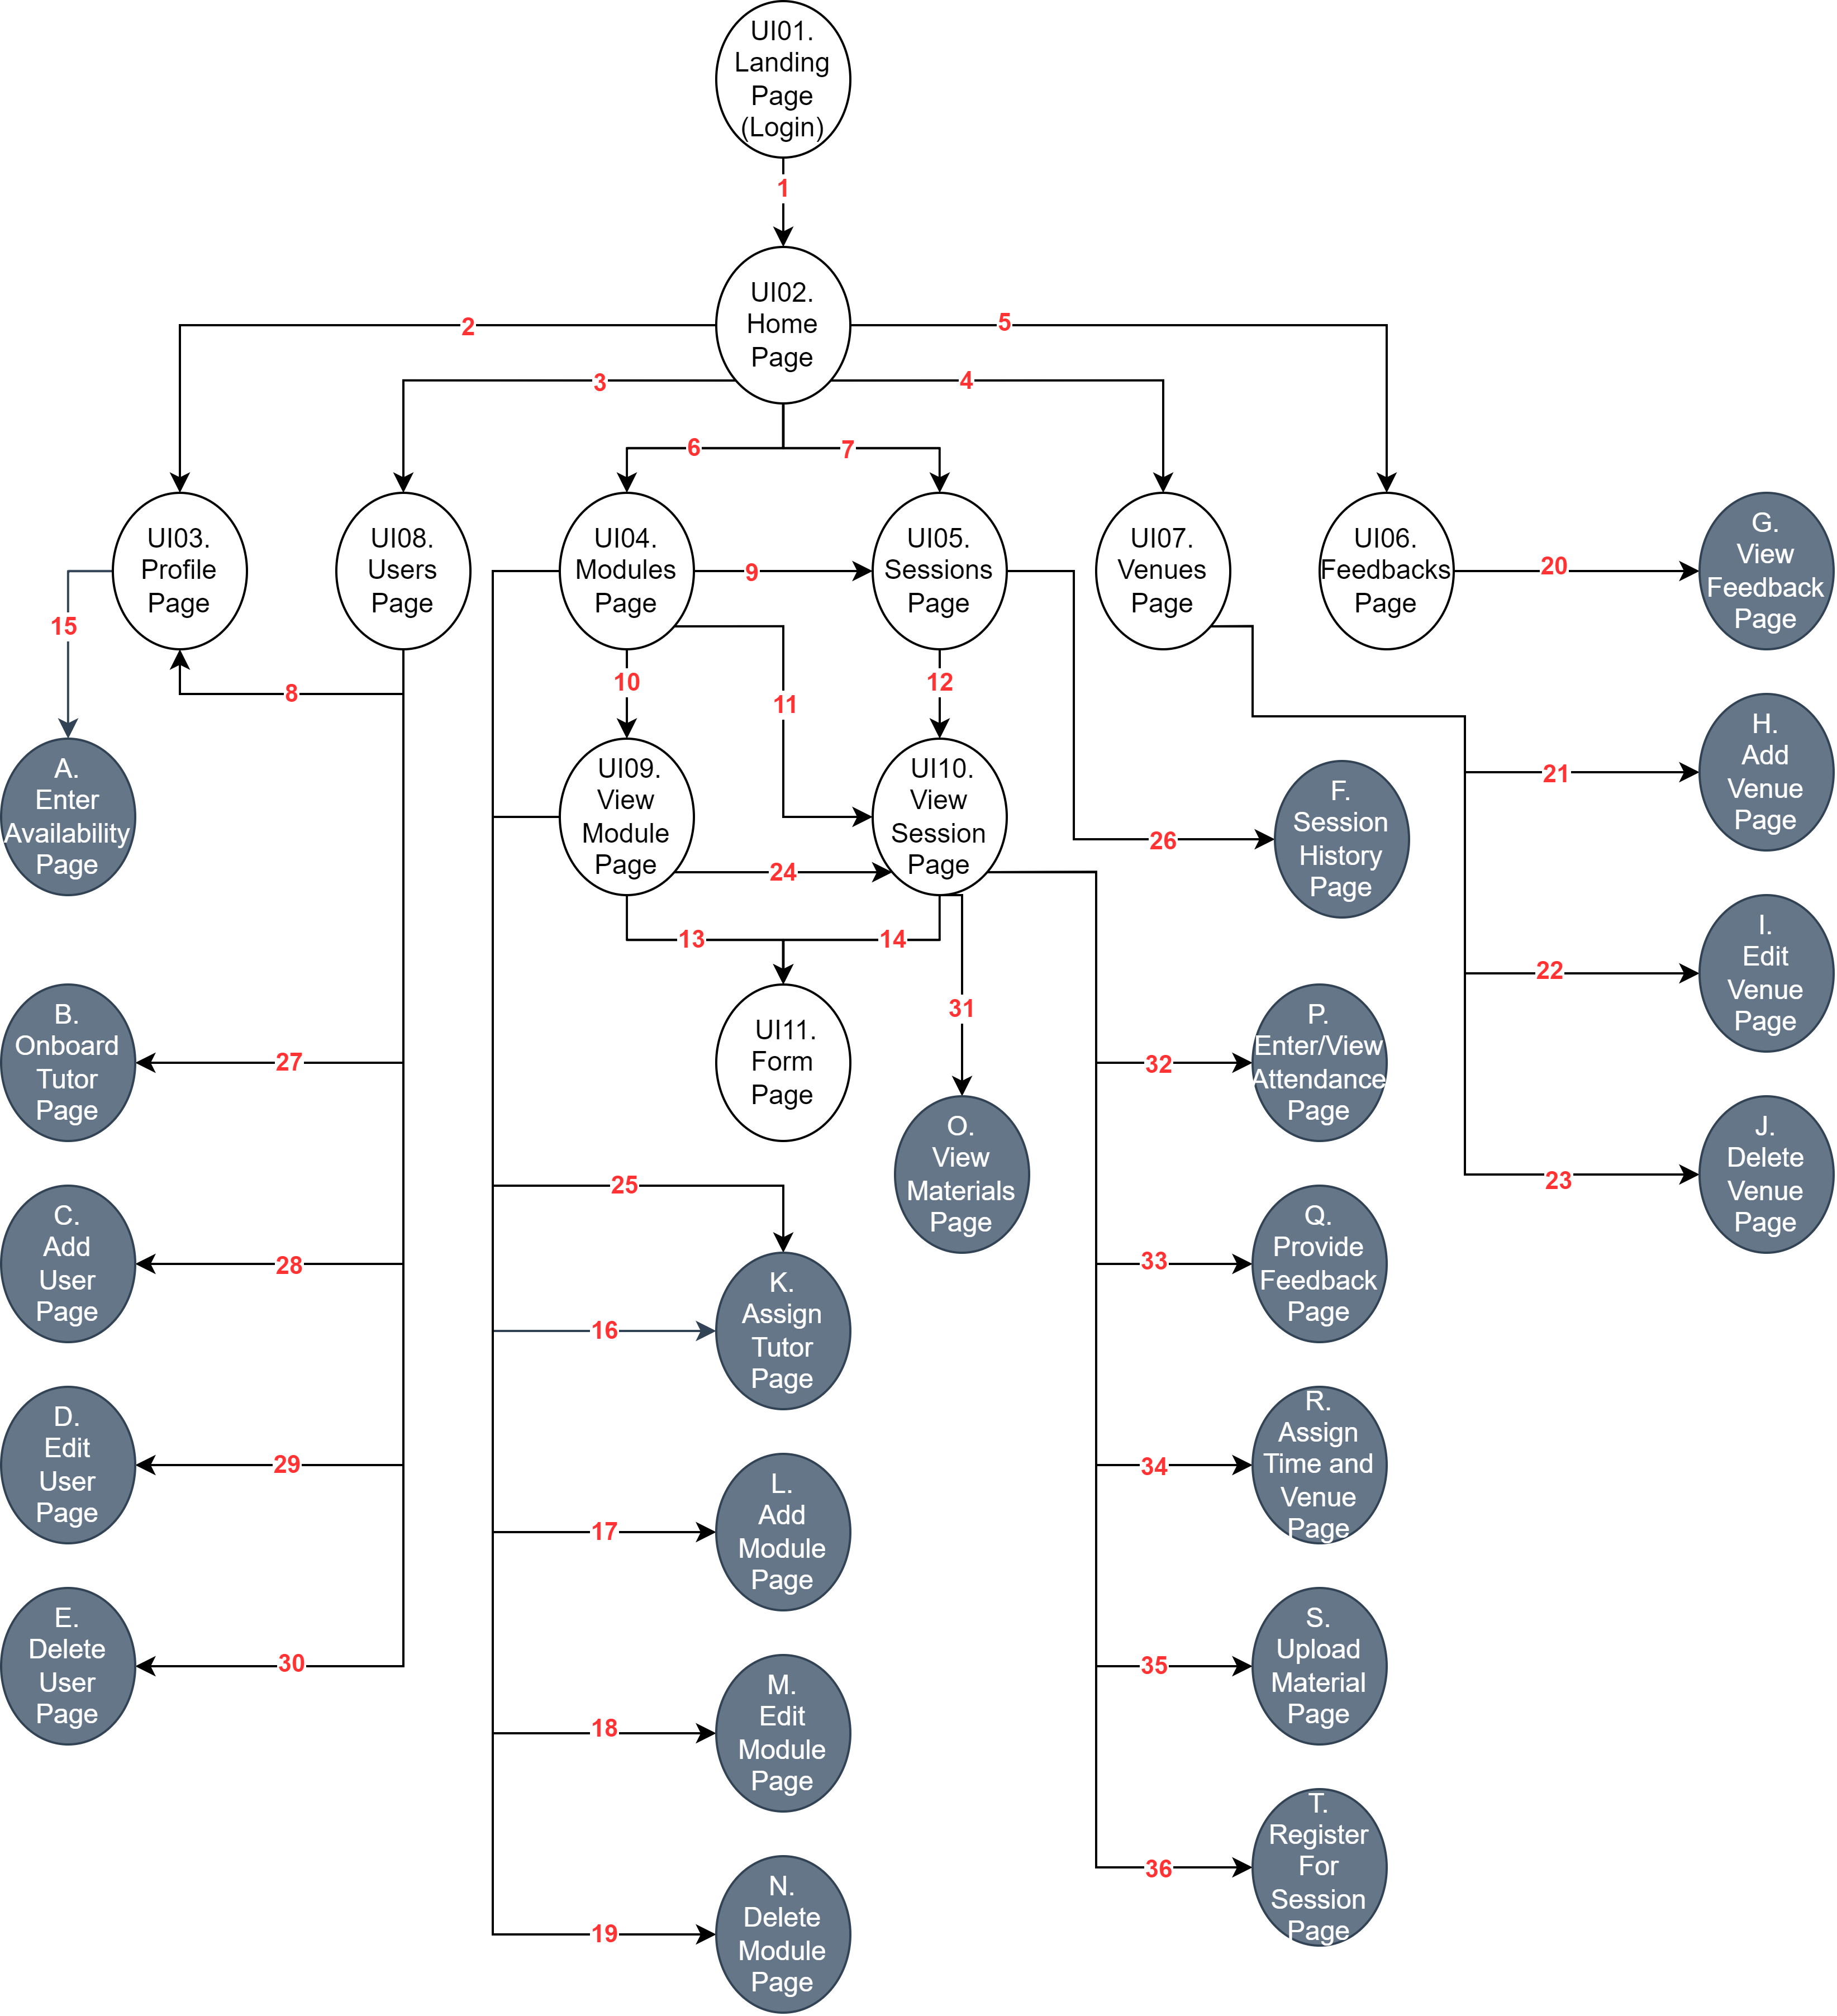
\includegraphics[width=150mm,scale=1]{figures/implementation_and_testing/testing/FSM/FSM.png}}
        \caption{FSM State Transitions}
        \label{FSM}
    \end{figure}
    
    \vspace{-0.5cm}
    \noindent The rows correspond to current states, while the columns indicate next states. The
    row/column intersections indicate actions associated with the state transitions. There are
    cases in which multiple different actions result in the same transition. The actions are enumerated and shown in Table \ref{FSMTable} presentation reasons. The N/A is an automated action that leads back to the UI11. Form Page since there are a lot of them, it is not shown in the diagram for simplicity. It is also worth mentioning that the A,B..T pages doesn't not have a specific UI designed for them in the previous chapter. However, they are known user interfaces that are form alike. The numbers on top are abbreviations like this UI01 => 1, UI07 => 7, and so on.

    \clearpage
    \begin{table}[H]
        \caption{FSM State Transition Table (c: current node, n: next node)}
        \begin{minipage}[trim]{1\textwidth}
        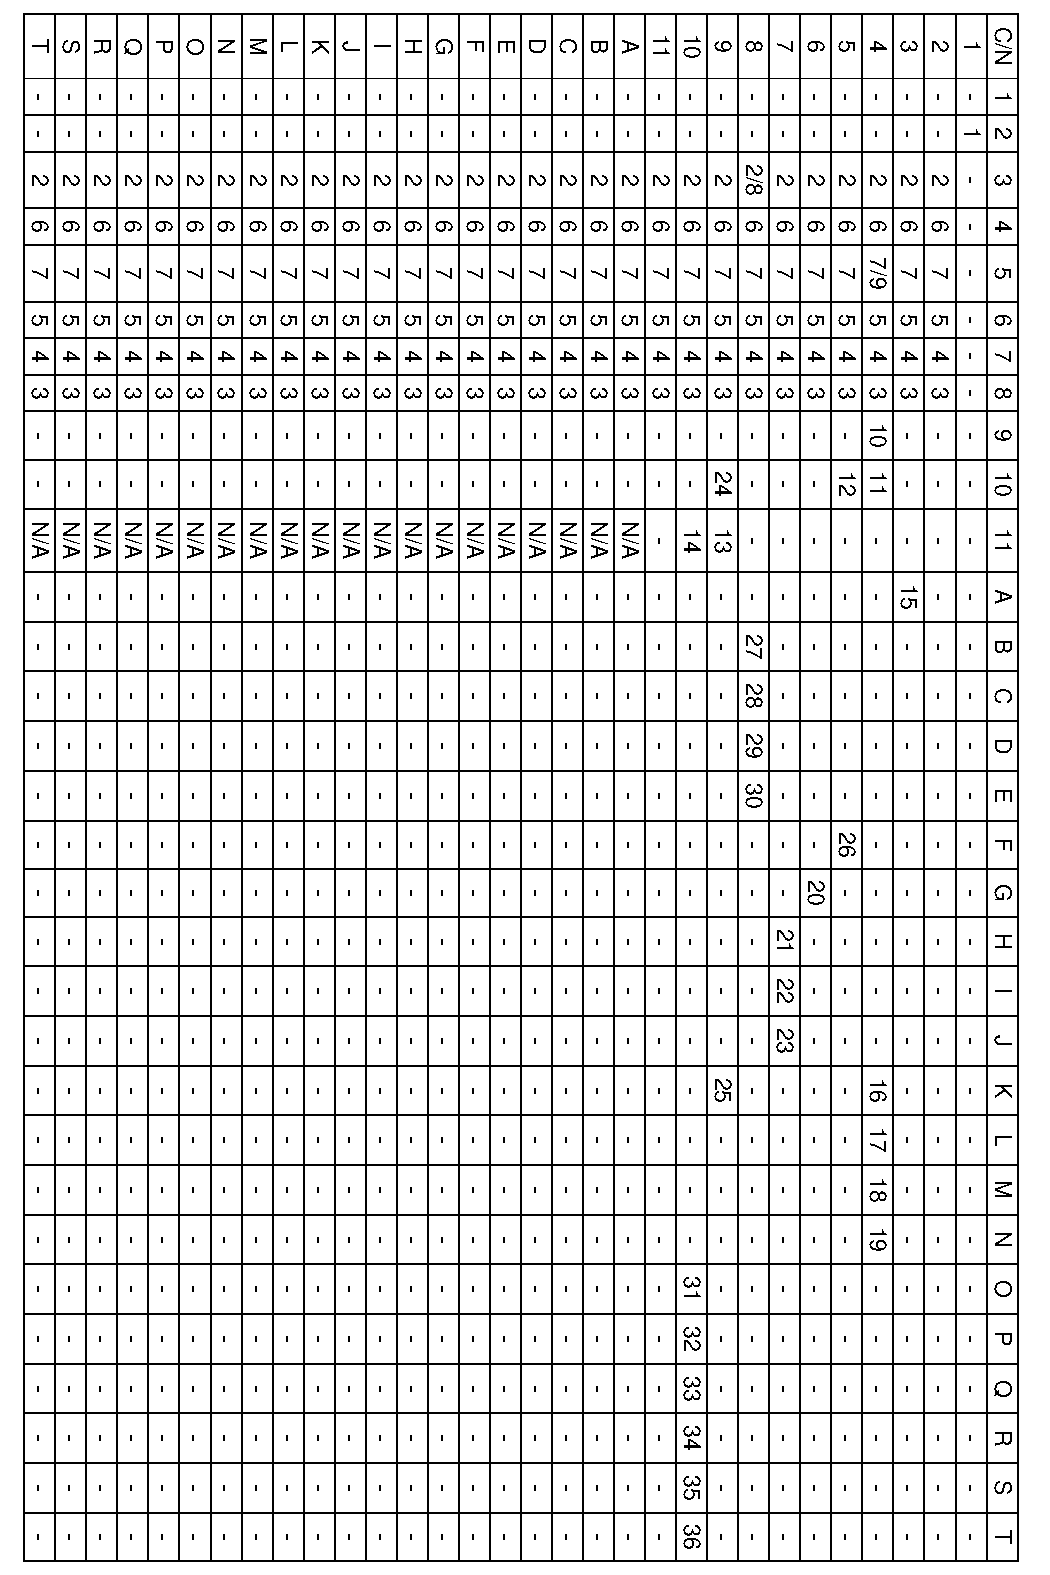
\includegraphics[width=\textwidth]{figures/implementation_and_testing/testing/FSM/fsm V1 (1).pdf}
        \end{minipage}
    \end{table}

    \renewcommand{\arraystretch}{0.8}
    \begin{table}[H]
        \centering
        \caption{Actions and their references}
        \begin{tabular}{|c|l|}
        \hline
        \rowcolor[rgb]{0.906,0.859,0.906} \textbf{ Action } & \textbf{ Reference }                                             \\
        \hline
        \textbf{ 1 }                                        & Login Button
          Click                                             \\
        \hline
        \textbf{ 2 }                                        & Profile
          Button Click from Sidebar                              \\
        \hline
        \textbf{ 3 }                                        & Users Button
          Click from Sidebar                                \\
        \hline
        \textbf{ 4 }                                        & Modules
          Button Click from Sidebar                              \\
        \hline
        \textbf{ 5 }                                        & Sessions
          Button Click from Sidebar                             \\
        \hline
        \textbf{ 6 }                                        & Venues Button
          Click from Sidebar                               \\
        \hline
        \textbf{ 7 }                                        & Feedbacks
          Button Click from Sidebar                            \\
        \hline
        \textbf{ 8 }                                        & Click on
          User’s Row in Users Page                              \\
        \hline
        \textbf{ 9 }                                        & View Sessions
          Button Click                                     \\
        \hline
        \textbf{ 10 }                                       & Click on
          Module’s Row from Modules Page                        \\
        \hline
        \textbf{ 11 }                                       & View Session
          Button Click from Module Page                     \\
        \hline
        \textbf{ 12 }                                       & View Session
          Button Click from Sessions Page                   \\
        \hline
        \textbf{ 13 }                                       & Assign Tutor
          Button Click from Module Page                     \\
        \hline
        \textbf{ 14 }                                       & Click on
          Session’s tab buttons                                 \\
        \hline
        \textbf{ 15 }                                       & Enter
          Availability Button from Profile Page                    \\
        \hline
        \textbf{ 16 }                                       & Assign Tutor
          Button Click from Modules Page                    \\
        \hline
        \textbf{ 17 }                                       & Add Button
          Click from Module Page                              \\
        \hline
        \textbf{ 18 }                                       & Edit Button
          Click from Module Page                             \\
        \hline
        \textbf{ 19 }                                       & Delete Button
          Click from Module Page                           \\
        \hline
        \textbf{ 20 }                                       & View Feedback
          Button from Feedbacks Page                       \\
        \hline
        \textbf{ 21 }                                       & Add Button
          Click from Venue Page                               \\
        \hline
        \textbf{ 22 }                                       & Edit Button
          Click from Venue Page                              \\
        \hline
        \textbf{ 23 }                                       & Delete Button
          Click from Venue Page                            \\
        \hline
        \textbf{ 24 }                                       & View Session
          Button Click from Module Page                     \\
        \hline
        \textbf{ 25 }                                       & Assign Tutor
          Button Click from Module Page                     \\
        \hline
        \textbf{ 26 }                                       & View Session
          History Button from Sessions Page                 \\
        \hline
        \textbf{ 27 }                                       & Onboard Tutor
          Button from Users Page                           \\
        \hline
        \textbf{ 28 }                                       & Add Button
          Click from User Page                                \\
        \hline
        \textbf{ 29 }                                       & Edit Button
          Click from User Page                               \\
        \hline
        \textbf{ 30 }                                       & Delete Button
          Click from User Page                             \\
        \hline
        \textbf{ 31 }                                       & Materials Tab
          Click from Session Page                          \\
        \hline
        \textbf{ 32 }                                       & Attendance
          Tab Click from Session Page                         \\
        \hline
        \textbf{ 33 }                                       & Provide
          Feedback Tab Click from Session Page                   \\
        \hline
        \textbf{ 34 }                                       & Assign Time
          and Venue Tab Click from Session Page              \\
        \hline
        \textbf{ 35 }                                       & Upload
          Material Tab Click from Session Page                    \\
        \hline
        \textbf{ 36 }                                       & Register Tab Click
          from Session Page                           \\
        \hline
        \textbf{ N/A }                                      & Not Available
          (Automated action that redirected to Form Page)  \\
        \hline
        \end{tabular}
        \label{FSMTable}
    \end{table}

\end{justify}

\clearpage

\vspace{0.25cm}
\subsection{Boundary Analysis Testing}
\begin{justify}
    In boundary analysis testing, inputs that define the 'boundaries' of a component's functionality are examined. These limits include minimum and maximum limits as well as all permitted values within that range. It is necessary to conduct boundary testing because errors tend to occur at the input domain's limits. In the context of the STDC, boundary analysis testing was performed on TextFields and any other user-input fields.

    \vspace{0.25cm}
    \newendline Throughout the testing of the STDC application, various input types demonstrated consistent behavior. These input categories were evaluated:\\

    \begin{enumerate}
        \item \textbf{Auto Complete Text Field:} These fields enable the user to browse for predetermined options. The user cannot select options that are not included in the list, thus encouraging data precision. It was observed that all Auto Complete Text Fields in the application exhibited consistent behavior.
        
        \item \textbf{Text Field:} This is one of the most frequently utilized STDC application components. Although the component functioned as anticipated, it lacked obvious boundary restrictions. The examined limits included:

            \begin{itemize}
                \item Empty Field: Users are not allowed to submit an empty field and are informed when a required field is left blank.
                \item Symbols: The field accepts all types of symbols.
                \item Integers: All integer inputs are accepted.
                \item Characters: The field accepts all characters.
                \item Allowed Length: There appeared to be no limit to the length of input, with the application accepting even 10,000-character-long course names. Thus it could result in the below undesired user interfaces.
            \end{itemize}

            
        \begin{figure}[H]
            \centerline{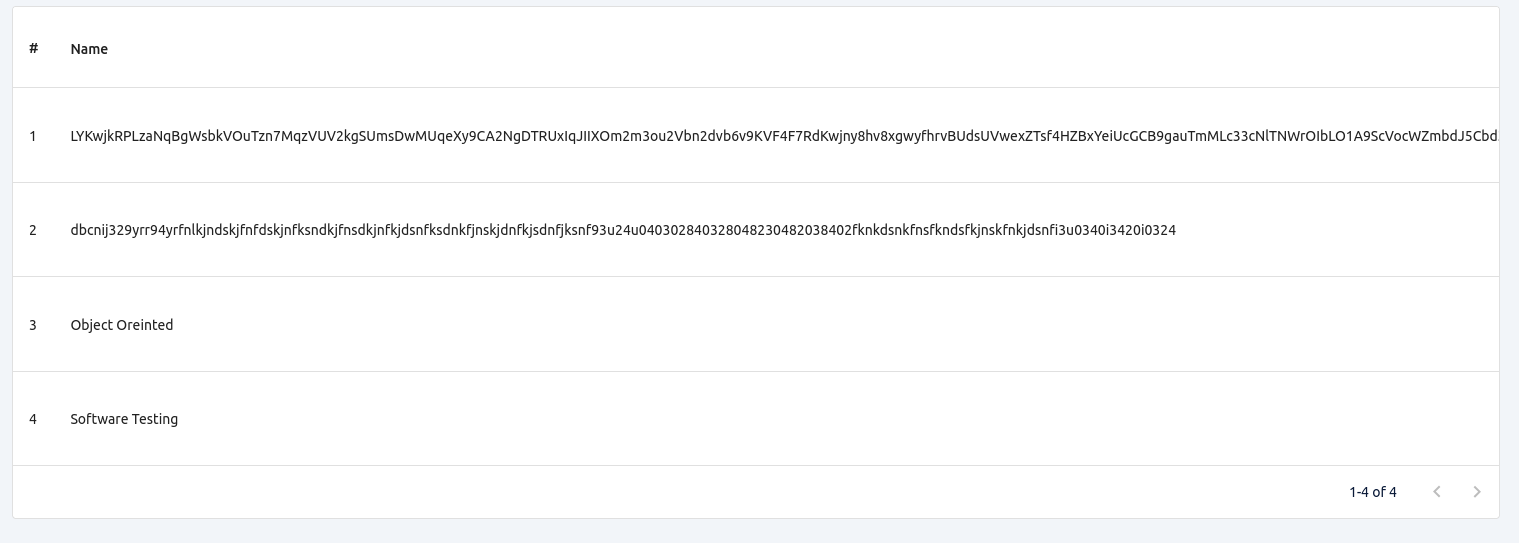
\includegraphics[width=150mm,scale=1]{figures/implementation_and_testing/testing/BAT/boundary (1).png}}
            \caption{Invalid course name in courses table}
            \label{invalid_course_name_table}
        \end{figure}

        \begin{figure}[H]
            \centerline{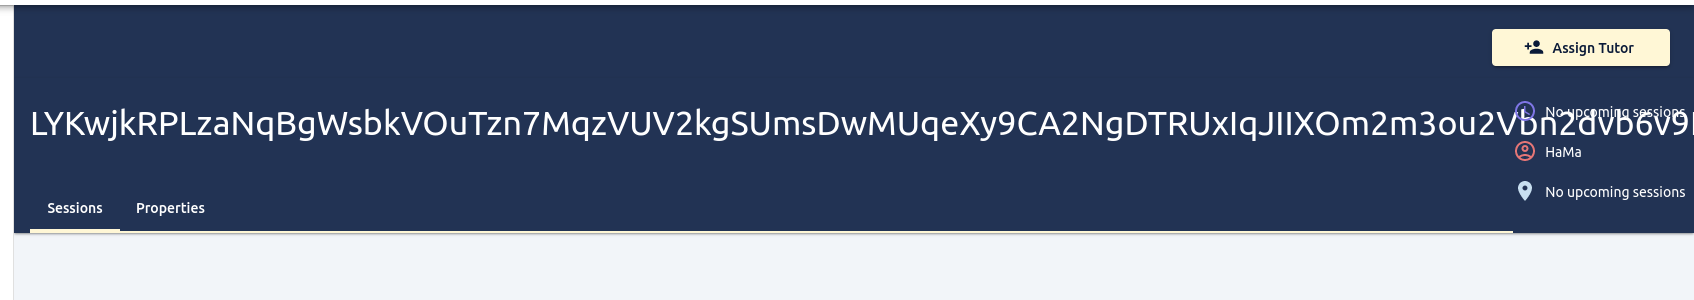
\includegraphics[width=150mm,scale=1]{figures/implementation_and_testing/testing/BAT/boundary (2).png}}
            \caption{Invalid course name in course profile}
            \label{invalid_course_name_profile}
        \end{figure}
        
        \item \textbf{File Upload:} This feature, available in the Resource Management System, allows users to upload any type of file, one at a time. A potential improvement could be to allow multiple file uploads simultaneously, which would enhance user experience and efficiency.

        \item \textbf{Selection:} This component functioned well, only allowing options within the predefined boundary to be selected.

        \item \textbf{Rating:} Users are permitted to select whole numbers between 1 and 5, with the system correctly prohibiting the selection of negative numbers or any numbers outside of the given range.

        \item \textbf{Date Picker:} Date pickers functioned well, disallowing the selection of past dates for future sessions and the selection of weekends. However, the system didn't prevent the selection of holidays, which could be a potential area of improvement.

        \vspace{2cm}

        \item \textbf{Time Picker:} These functioned efficiently, restricting time selection outside of the UKH's working hours (8 AM to 8 PM) and ensuring that the start time of a session wasn't later than the end time.

        \item \textbf{Numeric Text Field:} These were used exclusively in venue creation. The behavior of these fields was unusual:

        \begin{itemize}
            \item Character Input: As expected, character input wasn't allowed.
            \item Capacity Input: Users were able to enter a capacity of 0, a negative number, or even a number as high as 9999999999. This behavior is quite irregular and could be problematic as the typical capacity for a UKH venue ranges from 10 to 500.\\
        \end{itemize}

            \begin{figure}[H]
                \centerline{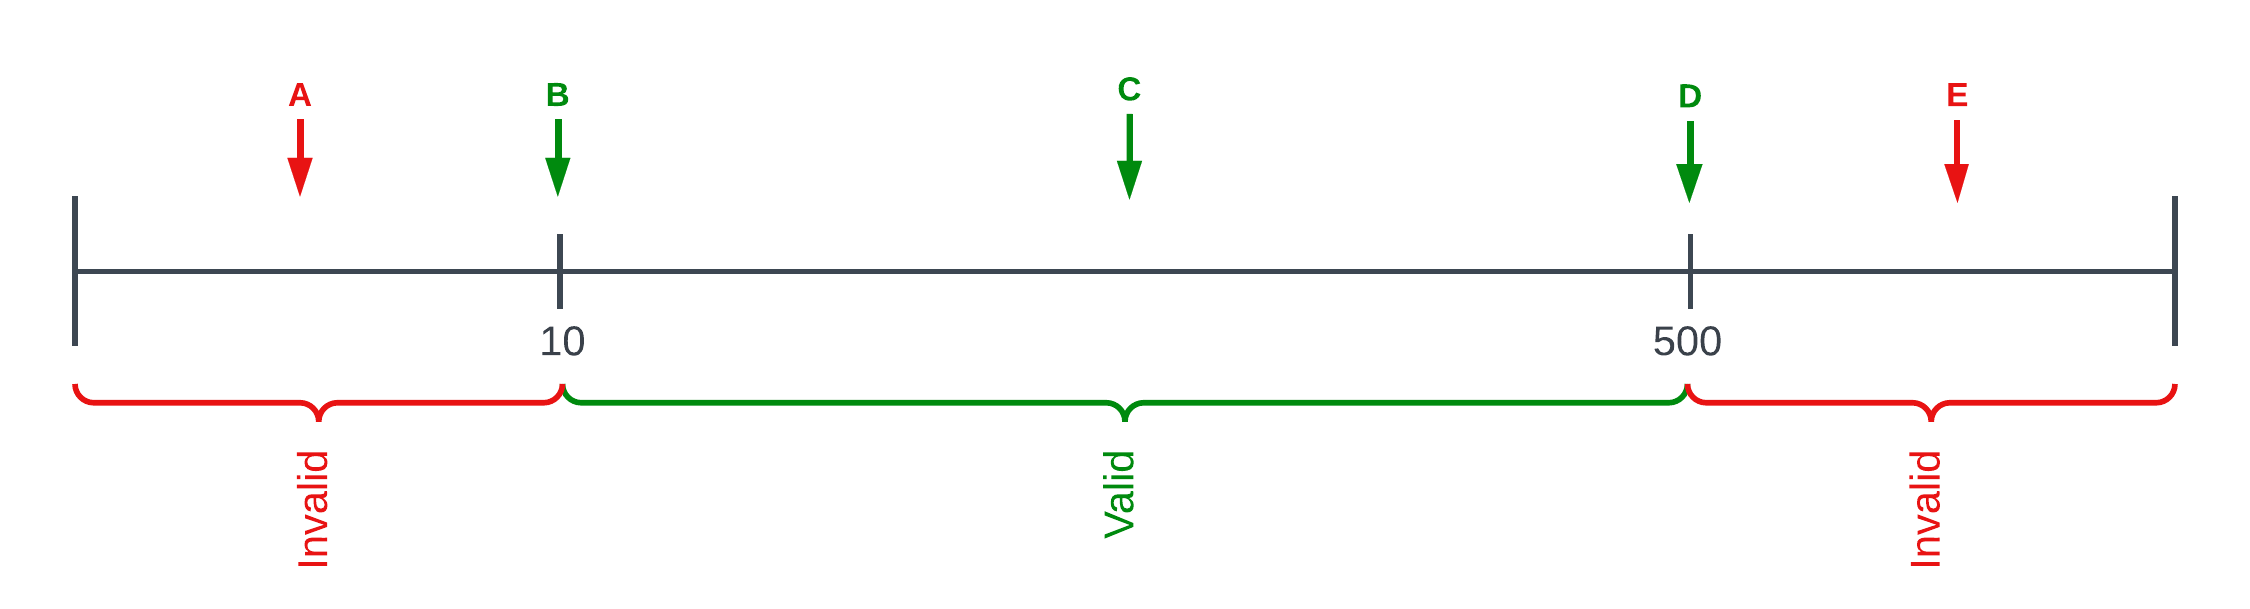
\includegraphics[width=150mm,scale=1]{figures/implementation_and_testing/testing/BAT/boundary (5).png}}
                \caption{Numeric boundary analysis}
                \label{Numeric_boundary_analysis}
            \end{figure}

            \begin{table}[H]
            \caption{Numeric boundary analysis - test cases' table}
            \centering
            \begin{tabular}{|c|c|} 
            \hline
            \rowcolor[rgb]{0.851,0.886,0.953} \textbf{Test Case} & \textbf{Result}                                \\ 
            \hline
            A                                                    & \textbf{\textcolor{red}{Invalid}}              \\ 
            \hline
            B                                                    & \textbf{\textcolor[rgb]{0,0.69,0.314}{Valid}}  \\ 
            \hline
            C                                                    & \textbf{\textcolor[rgb]{0,0.69,0.314}{Valid}}  \\ 
            \hline
            D                                                    & \textbf{\textcolor[rgb]{0,0.69,0.314}{Valid}}  \\ 
            \hline
            E                                                    & \textbf{\textcolor{red}{Invalid}}              \\
            \hline
            \end{tabular}
            \end{table}

            \begin{figure}[H]
                \centerline{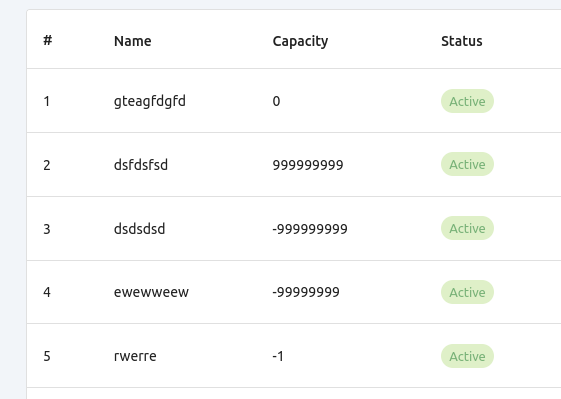
\includegraphics[width=120mm,scale=1]{figures/implementation_and_testing/testing/BAT/boundary (3).png}}
                \caption{Created venues with invalid capacities}
                \label{Numeric_boundary_analysis_venue_capacity}
            \end{figure}
    \end{enumerate}


    \newendline The results of boundary analysis testing for the STDC app showed how crucial it is to establish limits and boundaries in order to guarantee reliable data, enhance the user experience, and prevent bugs. Several potential enhancements were noted, including:\\

    \begin{itemize}
        \item One way to prevent users from entering unnecessarily long data is to enforce a maximum length for input in Text Fields.
        \item Adding the ability to upload several files at once to the File Upload function.
        \item Including minimum and maximum capacity validations in the Numeric Text Fields used for venue construction.
        \item To prevent the selection of holidays, a new validation should be added to the Date Picker.
    \end{itemize}


    \newendline As a result of resolving these findings and implementing the proposed enhancements, the STDC program will become more efficient and user-friendly. It highlights the value of boundary analysis testing in spotting vulnerabilities and making a program more stable.
\end{justify}
\clearpage

\vspace{0.25cm}
\subsection{Inspection Testing}
\begin{justify}
    During the course of an inspection test of the Student Talent Development Center (STDC) program, a number of major concerns were discovered, and the objective of this section is to offer a detailed explanation and evaluation of those issues. Because software reliability is essential to the usability and durability of a software application, such careful inspection tests are essential to find, explain, and then fix the many faults that could hinder the user experience. This is because software reliability is key to the usability and longevity of a software application.

    \vspace{0.25cm}
    \newendline In this section, we are going to concentrate on a manual inspection test, which entails doing a comprehensive investigation into the functioning of the system in order to locate any possible flaws or mistakes.

    \vspace{0.25cm}
    \newendline The STDC program was seen engaging in erroneous behavior on two separate occasions, both of which interfered with the software's capacity to perform its typical operations as described below. In the next section, we will examine each of these situations one at a time, providing specifics about the problem that arose, the investigation method that was utilized, the identification of the flaw, and the recommended solution.
    

    \vspace{0.25cm}
    \newendline \textbf{\textit{Case One: Tutor Login Issue}}\newendline
    The lack of ability of the application to authenticate a user who was attempting to log in with the role of "Tutor" was the first problem that was found during the manual inspection test. The authentication of users is the most important part of their interaction with the system; thus, this was a very serious issue.

    \vspace{0.25cm}
    \newendline When an attempt was made to log in as a Tutor, the system refused access. Further research using the network part of the browser's developer tool revealed that the "current-user" endpoint on the server had returned an error code of 401. This HTTP status code is typically sent in situations when authentication was requested but either failed or was not yet given. The fact that this error was generated suggested that the software was experiencing difficulties validating the user's login credentials.

    \begin{figure}[H]
        \centerline{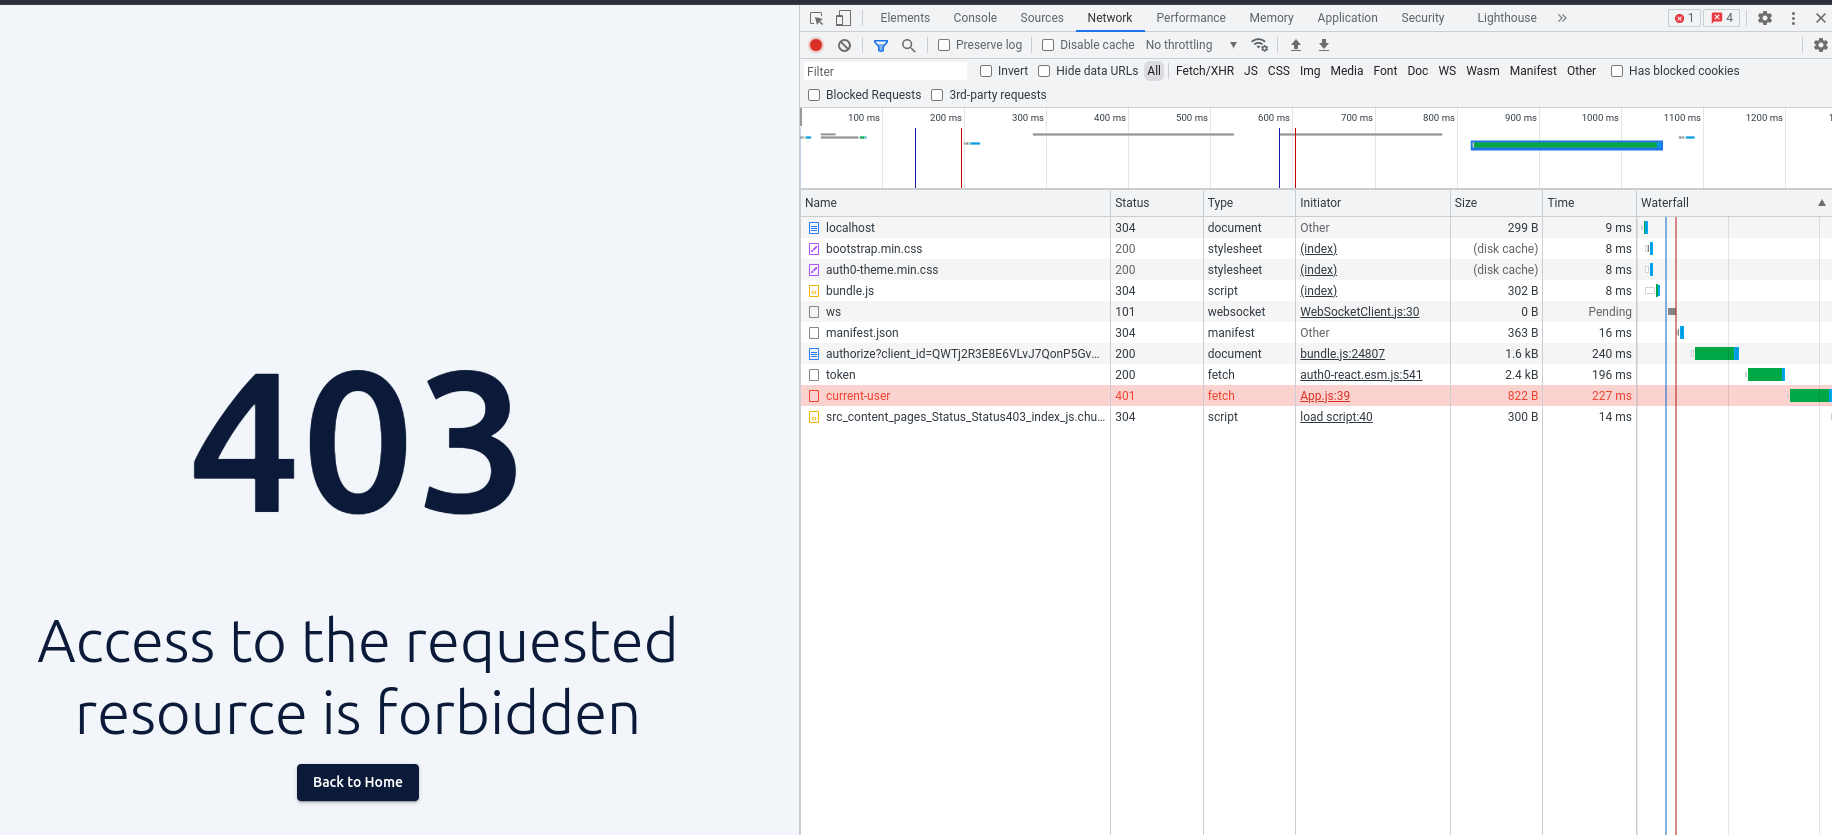
\includegraphics[width=150mm,scale=1]{figures/implementation_and_testing/testing/MIS/403.png}}
        \caption{Inspection testing - HTTP 403 when login}
        \label{Inspection_403}
    \end{figure}

    \vspace{0.25cm}
    \newendline In order to figure out what was causing this problem in the first place, the database that was hosted on the server had to be erased. This choice was made on the basis of the idea that an incorrect user object in the database may possibly be the cause of the issue. This step, however, inevitably led to another problem: the "Superadmin" user, who is immediately seeded into the database upon deployment and carries both the "Superadmin" and "Tutor" roles, was also unable to log in to the system. This user is automatically seeded into the database upon deployment.

    \vspace{0.25cm}
    \newendline Because the client was simply given a 401 Unauthorized error, it was determined that this problem should be investigated locally using the localhost. Copying the token that was used to log in as the superadmin user and using it for local testing was done so that the circumstances on the client side could be replicated.\\

    \vspace{0.25cm}
    \newendline During the course of the investigation, it was discovered that the error's stack trace led to the "ability.rb" model located in the models directory. The STDC application's user permissions are handled by this model, which is responsible for handling those permissions. Notably, if this file experiences an exception, it will send a 401 HTTP response by default. This explains both the server's 403 error and the client's 401 error when they try to retrieve current user information from the server.
%%%%%    
    \vspace{0.25cm}
    \newendline Following more investigation, the "tutor\_abilities" method was found to contain the problematic piece of code that was responsible for throwing the error. To be more specific, the program code attempted to retrieve the tutor ID from the tutor field of the user's record (which was a JSONB field in the database), compare it with the user's ID, but it failed to do so because of a syntax issue and instead raised an exception.

    \vspace{0.25cm}
    \newendline The incorrect line of code was: tutor[:id]: user.id, which indicated that the program was making an effort to get the id key from the tutor JSONB field and evaluate it in comparison to the user.id. Despite this,:tutor[:id]: was the source of an error since it had improper syntax. In addition, the user object wasn't created yet at that point in the code, which means that the user.id variable was also the source of the issue.

    \begin{figure}[H]
        \centerline{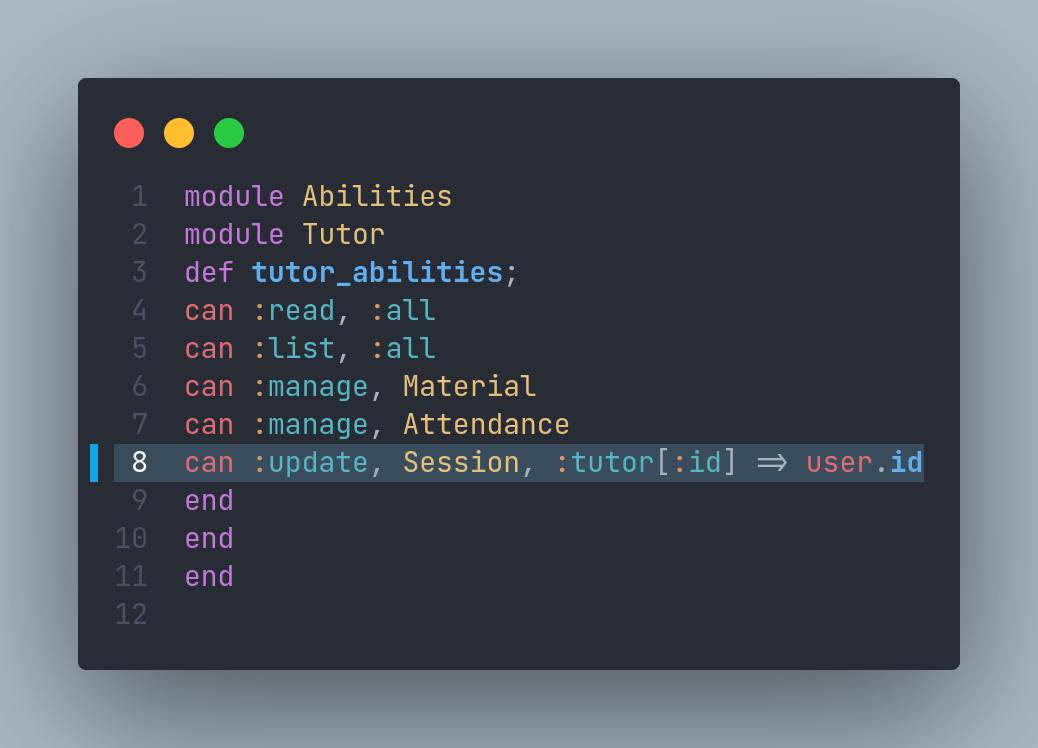
\includegraphics[width=150mm,scale=1]{figures/implementation_and_testing/testing/MIS/code_before.png}}
        \caption{Inspection testing - Case One Defected Line}
        \label{Inspection_403_defected_line}
    \end{figure}
    
    
    \vspace{0.25cm}
    \newendline The following is the implementation of the solution to correct this problem which is illustrated in the figure that can be seen below.

    \begin{figure}[H]
        \centerline{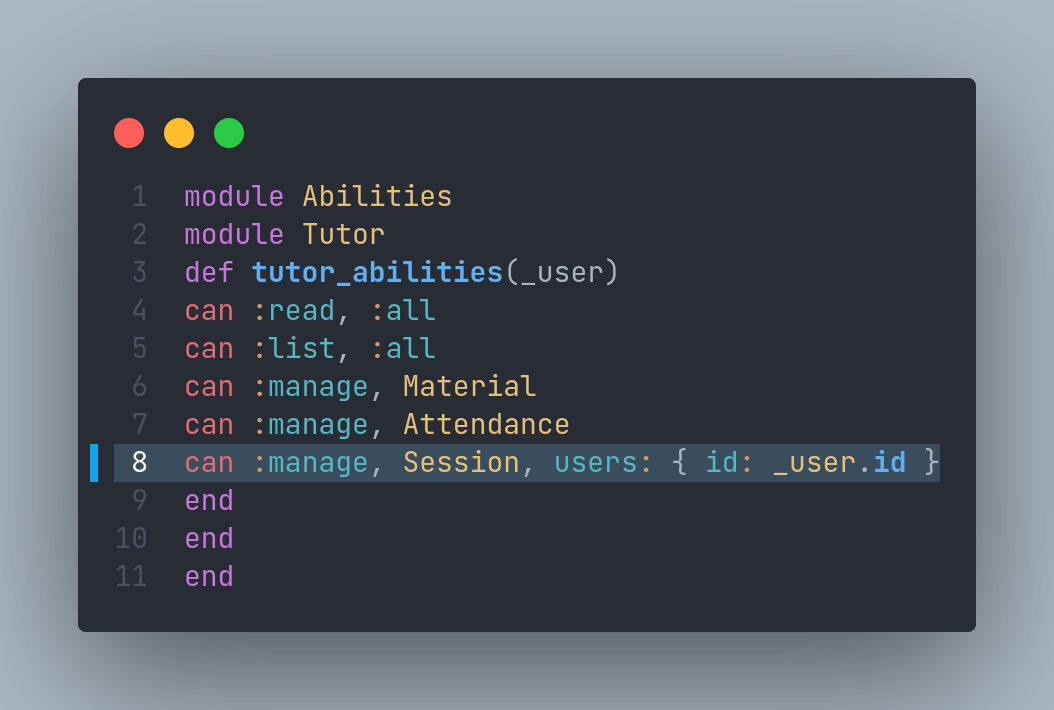
\includegraphics[width=150mm,scale=1]{figures/implementation_and_testing/testing/MIS/code.png}}
        \caption{Inspection testing - Case One Solution}
        \label{Inspection_403_solution}
    \end{figure}


    
    \vspace{0.25cm}
    \newendline \textbf{\textit{Case Two: Session Search Issue}}\newendline
    The lack of ability of the application to authenticate a user who was attempting to log in with the role of "Tutor" was the first problem that was found during the manual inspection test. The authentication of users is the most important part of their interaction with the system; thus, this was a very serious issue.

    \vspace{0.25cm}
    \newendline The second issue that we discovered during our inspection test relates to a problem with the search capability that can be found on the Sessions page. Within the STDC program, one of the most important functions is performed by the Sessions page, which displays all of the enrolled and readily available sessions. Users are given the ability to locate certain sessions in a timely manner thanks to the inclusion of a search bar on this page. However, during testing it was determined that this feature had a fundamental problem, which undermines the usability that was intended for the website.

    \vspace{0.25cm}
    \newendline When a user tries to find an existing session, the autocomplete function offers suitable session options depending on the keywords that have been typed. When a user clicks on a session from the search results, the functionality of this feature is supposed to take them to the page of the selected session. This is the intended behavior. Nevertheless, when testing, it was noticed that selecting a session result does not lead the user to the appropriate location when they click on it. Instead, it essentially fills the autocomplete search bar with the name of the selected session, keeping the user rooted on the Sessions page throughout the process.

    \begin{figure}[H]
        \centerline{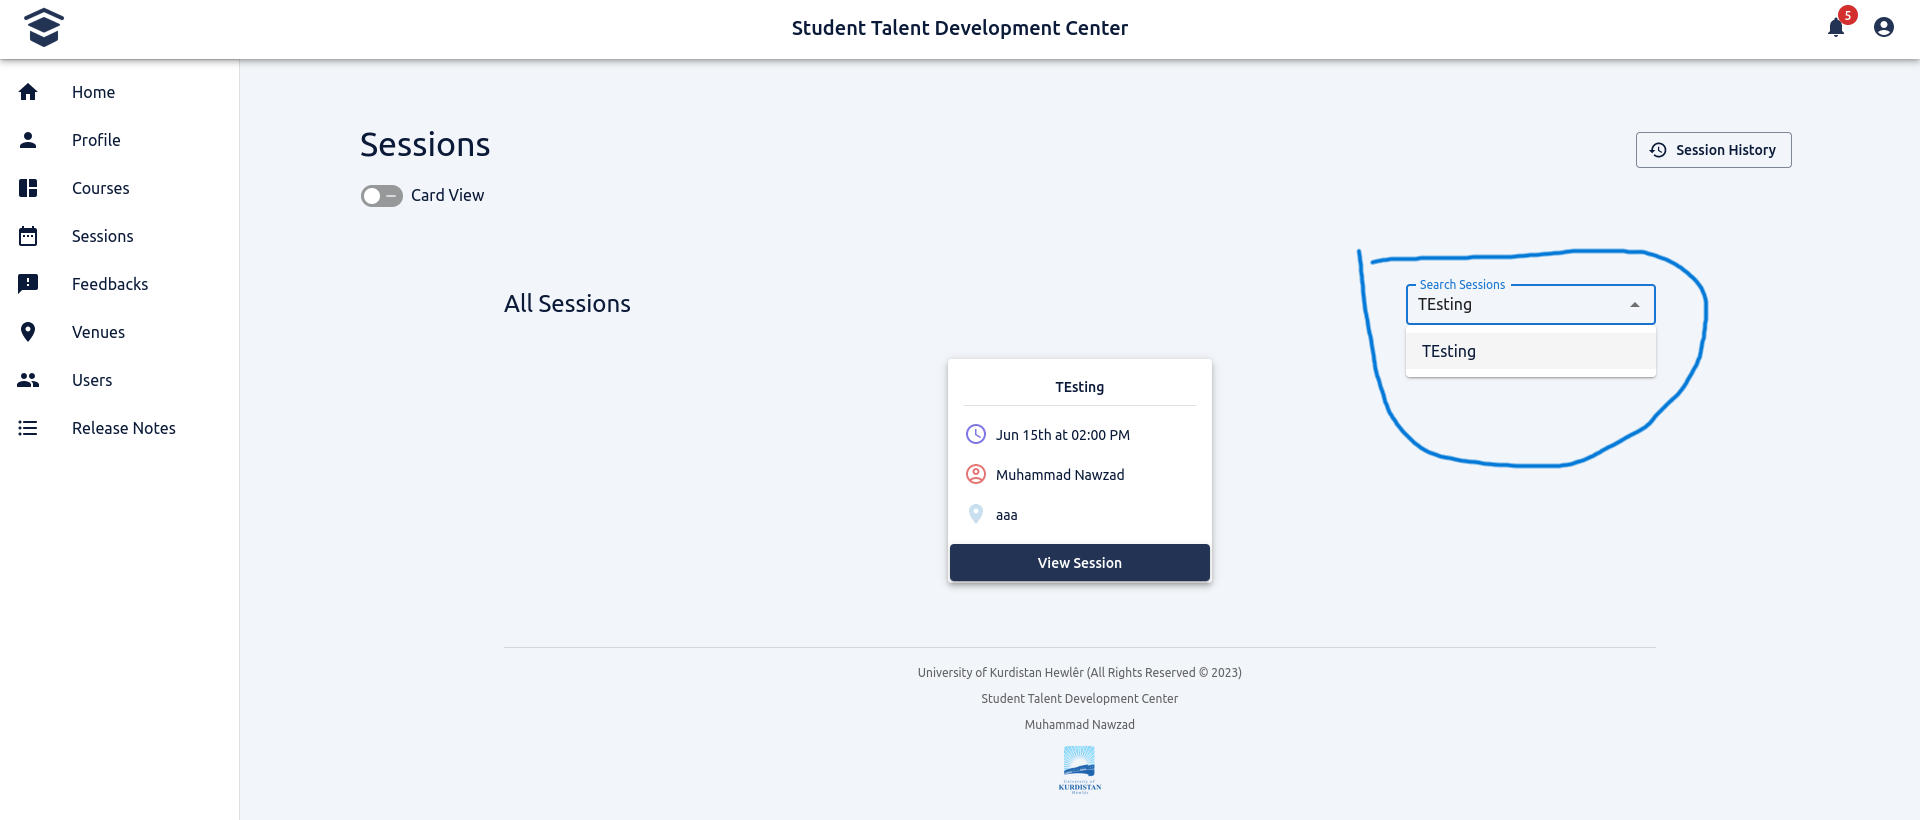
\includegraphics[width=150mm,scale=1]{figures/implementation_and_testing/testing/MIS/search.png}}
        \caption{Inspection testing - Case Two defective search}
        \label{Inspection_search}
    \end{figure}

    \vspace{0.25cm}
    \newendline This confusing problem called for a more thorough investigation of the onClick event that is connected to the search results. When a user clicks on a session name from the search results, this event is responsible for the action that is executed as a result of that click. It was thought that a mistake occurring during this moment may be the root cause of the observed dysfunction.

    \vspace{0.25cm}
    \newendline After doing an investigation into the code, it was found that the onClick event's method had been supplying inaccurate information on the session's redirect link. Due to the fact that this link was broken, the system was unable to properly redirect the user to the session page that they intended. The 'allSessions' useState, which is supposed to store all of the session information, was specifically built so that the link generating technique could access the session ID from there. On the other hand, because of a mistake in the coding, it was attempting to access the 'allCourses' useState instead, which is not declared in the file that is relevant to the discussion.

    \begin{figure}[H]
        \centerline{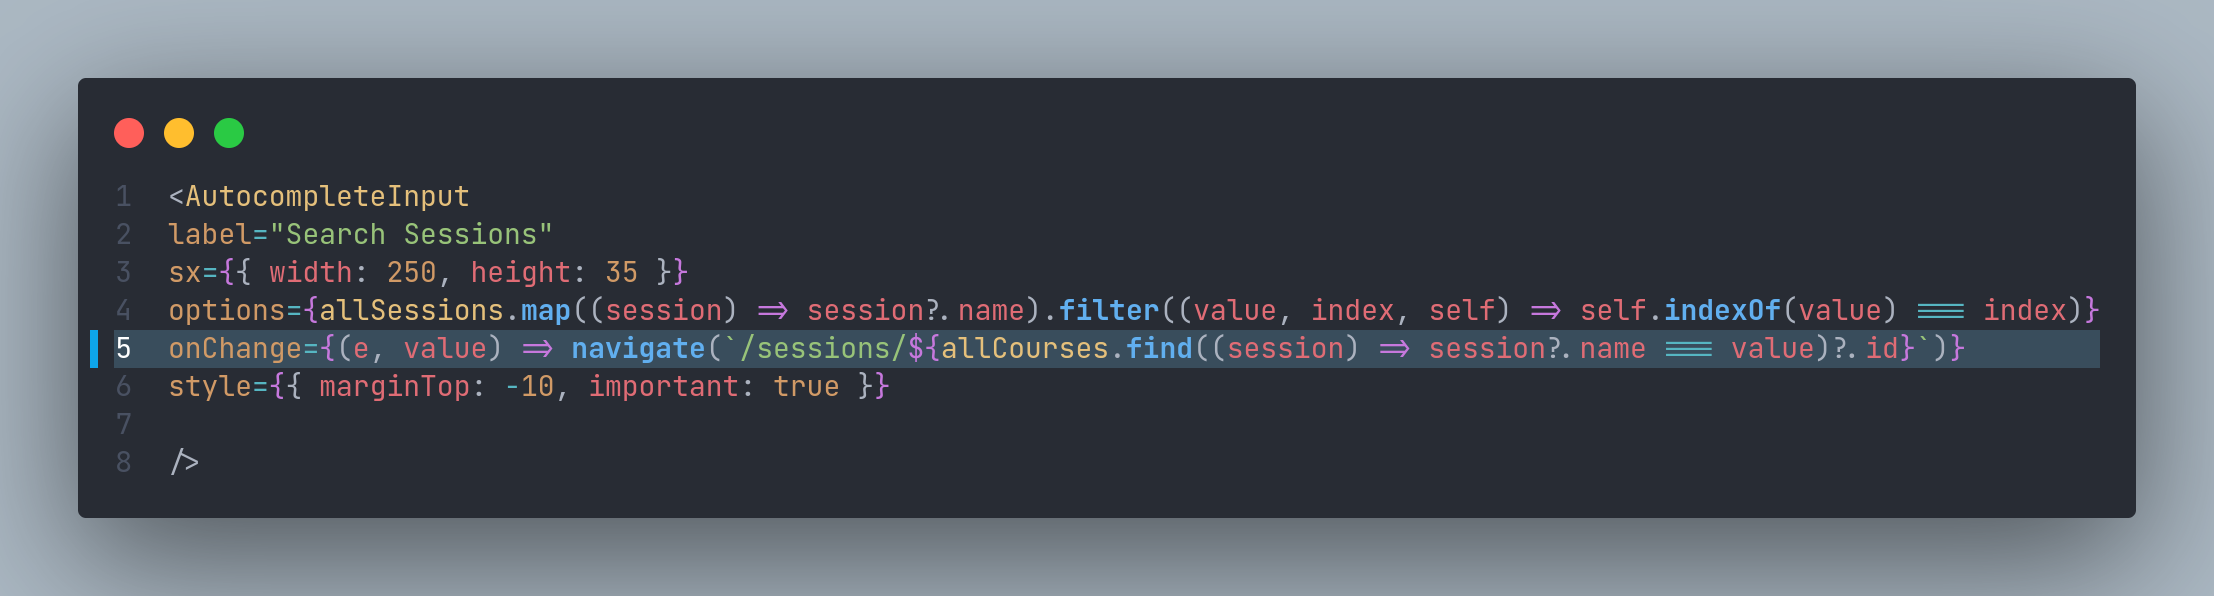
\includegraphics[width=150mm,scale=1]{figures/implementation_and_testing/testing/MIS/allcourses error.png}}
        \caption{Inspection testing - Case Two defected line}
        \label{Inspection_search_defect}
    \end{figure}

    \vspace{0.25cm}
    \newendline The answer to this situation was not overly complicated to figure out. The problem might be fixed by substituting the undefined 'allCourses' useState with the specified 'allSessions' useState instead. After making this adjustment, the functionality of the search box restored to how it should have been behaving. After the user makes their selection from the list of search results, they are immediately sent to the page that corresponds to the selected session.

    \vspace{0.25cm}
    \newendline The solution to this problem is illustrated in the figure below.
    
    \begin{figure}[H]
        \centerline{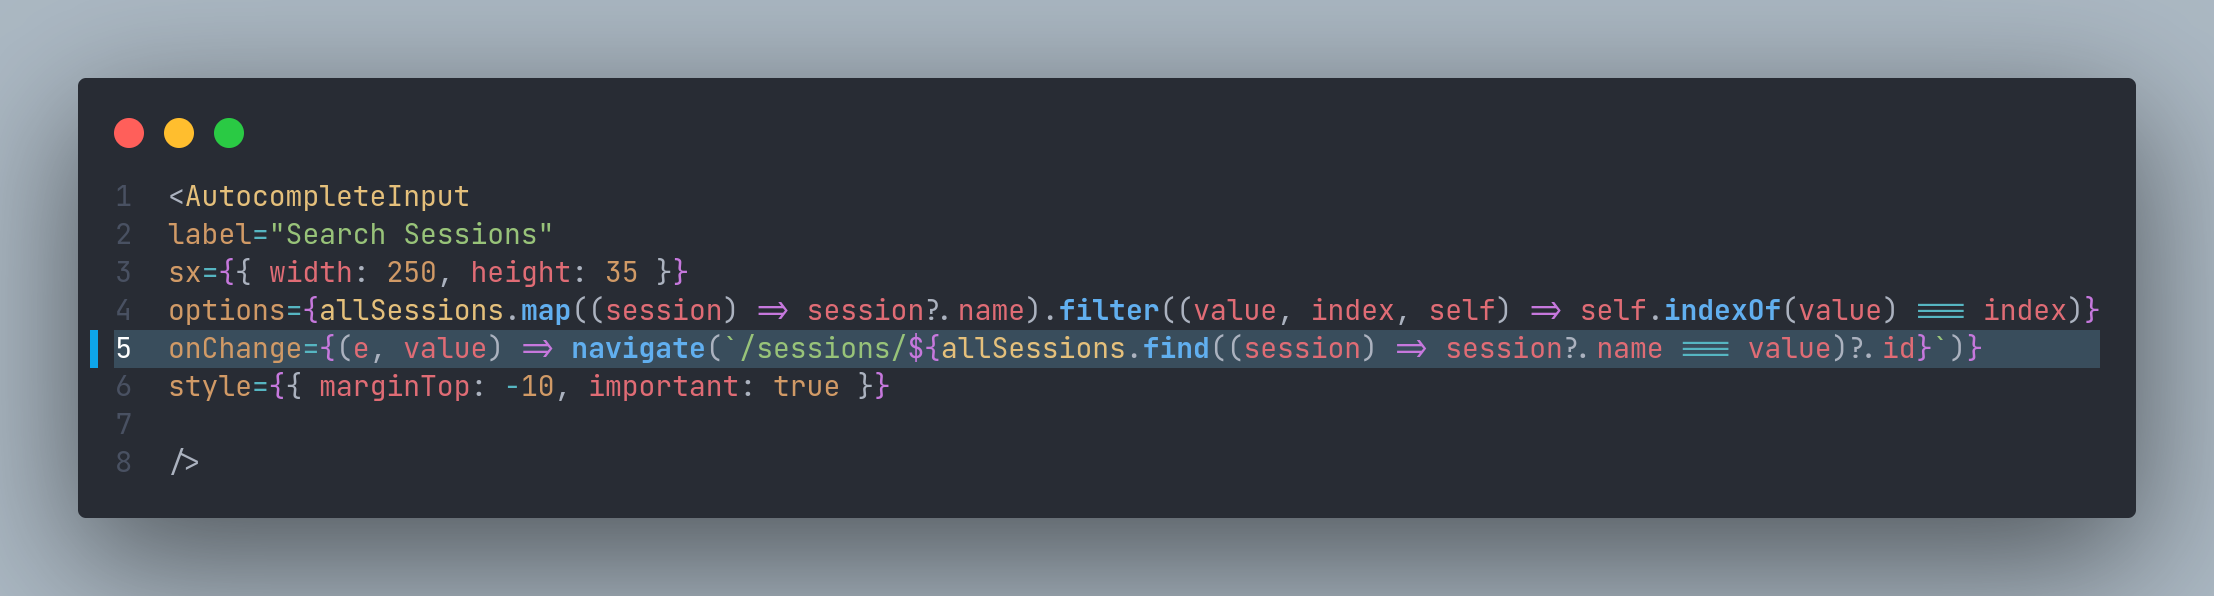
\includegraphics[width=150mm,scale=1]{figures/implementation_and_testing/testing/MIS/allcourses error fix.png}}
        \caption{Inspection testing - Case Two Solution}
        \label{Inspection_search_defect_fix}
    \end{figure}

    
    \clearpage
    \newendline \textbf{\textit{Summary}}\newendline
    During the course of the manual inspection test, we found two major issues with the STDC application. The need of thorough testing in the field of software development is made clear by both of these examples. Problems with the login process or the search bar can have a significant impact on how the program works for its users. By carefully examining these instances, we may not only pinpoint the issues but also discover their causes, leading to a deeper comprehension of the system as a whole.

    \vspace{0.25cm}
    \newendline First, we looked at a serious vulnerability that was preventing a 'Tutor' user from signing in. After discovering this problem, we dug into the server's responses, inspected the database, and studied the error stack trace in great detail. We tracked down the cause of the login problem to a syntax error in the 'tutor\_abilities' function of the 'ability.rb' model. The error was caused by a call to a non-existent object, 'user.id', which was intended to compare the value of the 'id' field in the JSONB tutor object to a value outside the function's scope. By fixing this problem, we were able to bring back a crucial part of the app's operation, login.
    
    \vspace{0.25cm}
    \newendline The second scenario required us to investigate a malfunctioning search feature on the 'Sessions' page. While the search bar is a vital navigational aid, it was not properly taking users to the appropriate session page. We discovered the session's redirect URL was incorrectly produced during our onClick investigation because the software was trying to retrieve data from an undefined useState. A straightforward yet possibly irritating oversight was uncovered by this investigation. We were able to get the search bar working again after a fast patch of changing the incorrect useState with the proper one.
    
    \vspace{0.25cm}
    \newendline The complexity and interdependence of the many parts of a software program are shown by these two examples. A single mistake in the code might have a domino effect, resulting in serious problems that affect the program as a whole. This highlights the significance of thorough testing and inspection. By thoroughly testing the system, we can guarantee that the final product will be dependable, effective, and simple to use.

\end{justify}
\clearpage



%%%%%%%%%%%%%%%%%%%%%%%%%%%%%%%%%%%%%%%%%%%%%%%%%%%%%%%%%%%%%%%%%
%%%%%%%%%%%%%%%%%%%%%%%%%%%%%%%%%%%%%%%%%%%%%%%%%%%%%%%%%%%%%%%%%
%%%%%%%%%%%%%%%%%%%%%%%%%%%%%%%%%%%%%%%%%%%%%%%%%%%%%%%%%%%%%%%%%
%%%%%%%%%%%%%%%%%%%%%%%%%%%%%%%%%%%%%%%%%%%%%%%%%%%%%%%%%%%%%%%%%



\vspace{0.25cm}
\subsection{Granularity of Automated Testing}
\begin{justify}
Automated testing plays a crucial role in the development and deployment of high-quality, dependable software, reducing the likelihood of unanticipated behavior or defects once the software reaches end-users. In this section, we will examine the Student Talent Development Center's (STDC) automated testing procedures.


\vspace{0.25cm}
\newendline The STDC application consists of four primary components: the Core System, the Feedback System, the Resource Management System, and the Scheduling System. The Core System component is at the core of the application, comprising fundamental features such as user management. The Feedback System functions as a mechanism for collecting user feedback, thereby facilitating the continuous refinement and enhancement of the user experience. The Resource Management System facilitates course and session content management and uploading. Lastly, the Scheduling System assists in coordinating and managing the scheduling of various events and duties within the application.

\vspace{0.25cm}
\newendline Granularity in the context of automated testing refers to the level of specificity or detail at which testing is conducted. Granularity within the STDC application has been established at two distinct levels: the method level for unit testing and the class level for integration testing.

\vspace{0.25cm}
\newendline Unit testing is a testing strategy that entails testing individual software components, in this instance the class methods. The purpose of unit testing is to isolate a section of code and validate its correctness, enabling developers to detect flaws early in the development cycle and repair them more easily than if they were found later. Unit tests for STDC were written at the method level, concentrating on the simplest testable software component. This procedure ensures that each method, or mini-routine, in the software operates as expected.

\vspace{0.25cm}
\newendline Unit testing for the STDC application included a comprehensive examination of validations, enums, and associations. Using Rails as the framework and Rspec as the testing tool, unit testing confirmed that the methods adhered to the specified rules or 'validations', ensuring that the software would not accept invalid data. It ensured that 'enums', constants with a fixed set of predefined values, functioned accurately by testing them. The 'associations', or relationships between distinct classes in the software, were also examined to validate that the intended interactions between classes occurred. This method-level granularity of unit testing facilitated an inter-class testing scenario, permitting a thorough examination of the interactions between classes.

\vspace{0.25cm}
\newendline Integration testing, however, is a higher level than unit testing. It is a method of testing that verifies the compatibility of distinct software components when combined. In the STDC application, integration testing was conducted at the class level, with a focus on the interaction between classes within a component.

\vspace{0.25cm}
\newendline This level of granularity demands an in-depth understanding of how classes interact, given that a class may contain numerous methods. The integration tests for STDC focused mainly on testing all of the controller endpoints, or the numerous 'entry points' through which users interface with the application.

\vspace{0.25cm}
\newendline This form of integration testing also involved component-to-component interaction. Components, in terms of STDC's architecture, are collections of classes that deliver specialized system functionality. As classes within these components communicated with one another during testing, the application demonstrated inter-component communication. This allowed the identification and correction of any problems that could have arisen when classes from different components interacted, ensuring seamless coordination within the STDC application.

\vspace{0.25cm}
\newendline In conclusion, the STDC application's implementation of automated testing has been carefully planned with a keen focus on granularity. Method-level granularity in unit testing allowed for a detailed, micro-level perspective, facilitating the identification and resolution of issues within the application's methods. Class-level granularity in integration testing provided a macro-level perspective and ensured the seamless interaction and integration of various components. Consequently, by leveraging this multi-level granularity in automated testing, the STDC application demonstrates a robust, dependable software development strategy, preserving the quality and efficiency that are essential in today's rapidly evolving technology landscape.
\end{justify}
\clearpage


\vspace{0.25cm}
\subsection{Unit Testing}
\begin{justify}
Unit testing is a crucial aspect of testing of the Student Talent Development Center (STDC), offering a mechanism to validate the correctness and functionality of individual units within the application. Since STDC's backend uses the Ruby on Rails framework, these units are represented by the models, which are responsible for data management, business logic execution, and relationship mapping with other objects. Here, we will explore the unit testing strategies applied to our key models. The testing is facilitated by the RSpec testing framework, enhanced by the Shoulda Matchers library, which aids in creating clean, readable, and effective test cases.

\vspace{0.25cm}
\newendline \textbf{\textit{Common Testing Aspects}}\newendline
Both attribute validations and model associations are performed on every model. In order to guarantee that the model's data attributes are correct, attribute validations are performed. On the other hand, model associations are used to set up and confirm the connections between the various models in the system. In addition to associations and associations, in each model creation of an instance of that model is tested by using the subject which will contain an instance of the model if the build of that model is complete.


%%%%%%%%%%%%%%%%%%%%%%%%%%%%%%%%%%%%%%%%%%%%%%%%%%%%%%%%%%%%%%%%%
%%%%%%%%%%%%%%%%%%%%%%%%%%%%%%%%%%%%%%%%%%%%%%%%%%%%%%%%%%%%%%%%%

\vspace{0.25cm}
\newendline \textbf{\textit{User Model}}\newendline
The unit tests that have been completed for the User model are as follows.

\vspace{0.25cm}
\newendline
\textbf{Attribute Validations}

    \begin{figure}[H]
        \centerline{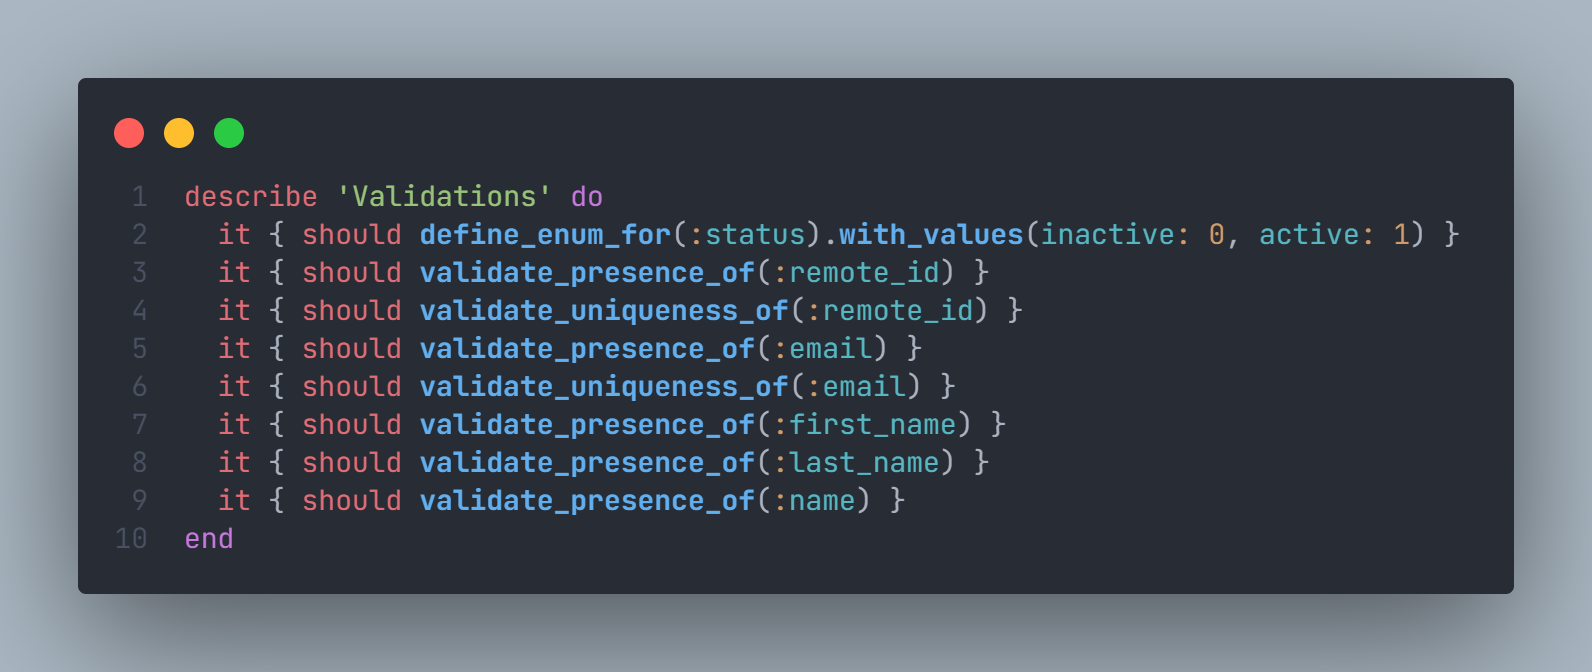
\includegraphics[width=140mm,scale=1]{figures/implementation_and_testing/testing/AUT/user/validations.png}}
        \caption{User Model - Validation Unit Tests}
        \label{User Model - Validation Unit Tests}
    \end{figure}


\vspace{0.25cm}
\noindent\noindent\textbf{\textit{\underline{Presence validation:}}} The validate\_presence\_of tests confirm that certain attributes must contain values. For example, validate\_presence\_of(:email) verifies that a User instance cannot be saved without an email attribute.

\vspace{0.25cm}
\noindent\textbf{\textit{\underline{Uniqueness validation:}}} These tests validate that the value of certain attributes is unique across all instances of a model, ensuring that no two users can share the same value of such an attribute. For instance, validate\_uniqueness\_of(:email) asserts that each User has a unique email.

\vspace{0.25cm}
\noindent\textbf{\textit{\underline{Enumeration validation:}}} We use define\_enum\_for to validate enumerations, where a set of named values correspond to integer values in the database. Our test, define\_enum\_for(:status).with\_values(inactive: 0, active: 1), confirms that the status attribute accurately maps the terms inactive and active to 0 and 1, respectively.

\vspace{0.25cm}
\newendline
\textbf{Model Associations}

    \begin{figure}[H]
        \centerline{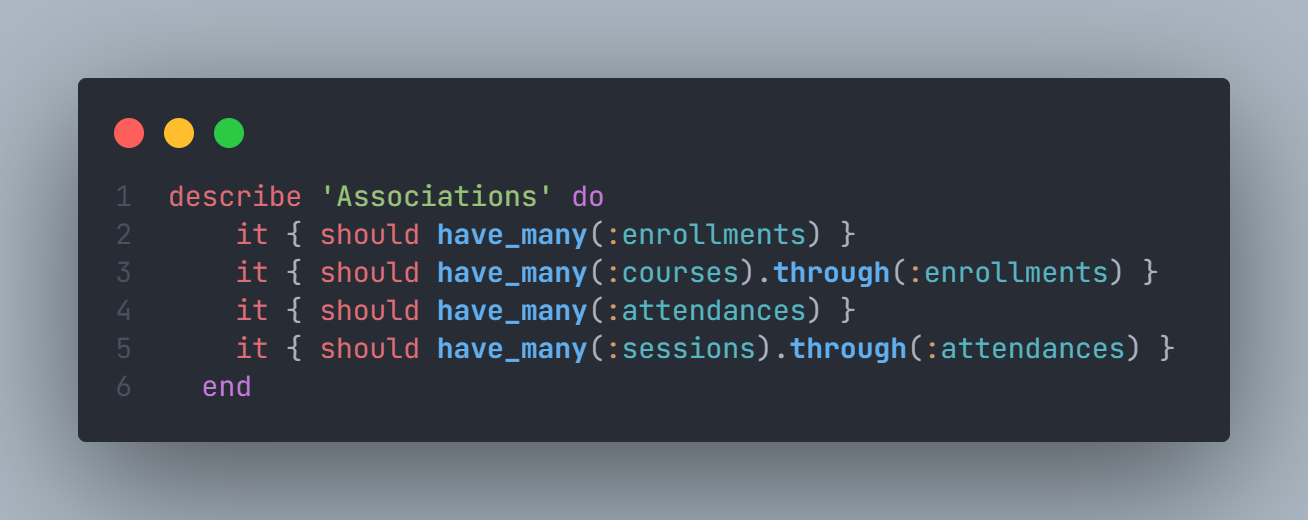
\includegraphics[width=140mm,scale=1]{figures/implementation_and_testing/testing/AUT/user/associations.png}}
        \caption{User Model - Association Unit Tests}
        \label{User Model - Association Unit Tests}
    \end{figure}

\vspace{0.25cm}
\noindent\textbf{\textit{\underline{One-to-many relationships:}}} The have\_many test verifies that one instance of the User model can be associated with multiple instances of another model. In our test suite, it { should have\_many(:enrollments) } and it { should have\_many(:attendances) } confirm that a User can have multiple Enrollments and Attendances, respectively.

\vspace{0.25cm}
\noindent\textbf{\textit{\underline{Many-to-many relationships:}}} The have\_many...through test validates relationships where a User instance can be associated with many instances of another model through a third model. In our suite, it { should have\_many(:courses).through(:enrollme- nts) } and it { should have\_many(:sessions).through(:attendances) } asserts that a User can be associated with many Courses through Enrollments, and with many Sessions through Attendances.


    \begin{figure}[H]
        \centerline{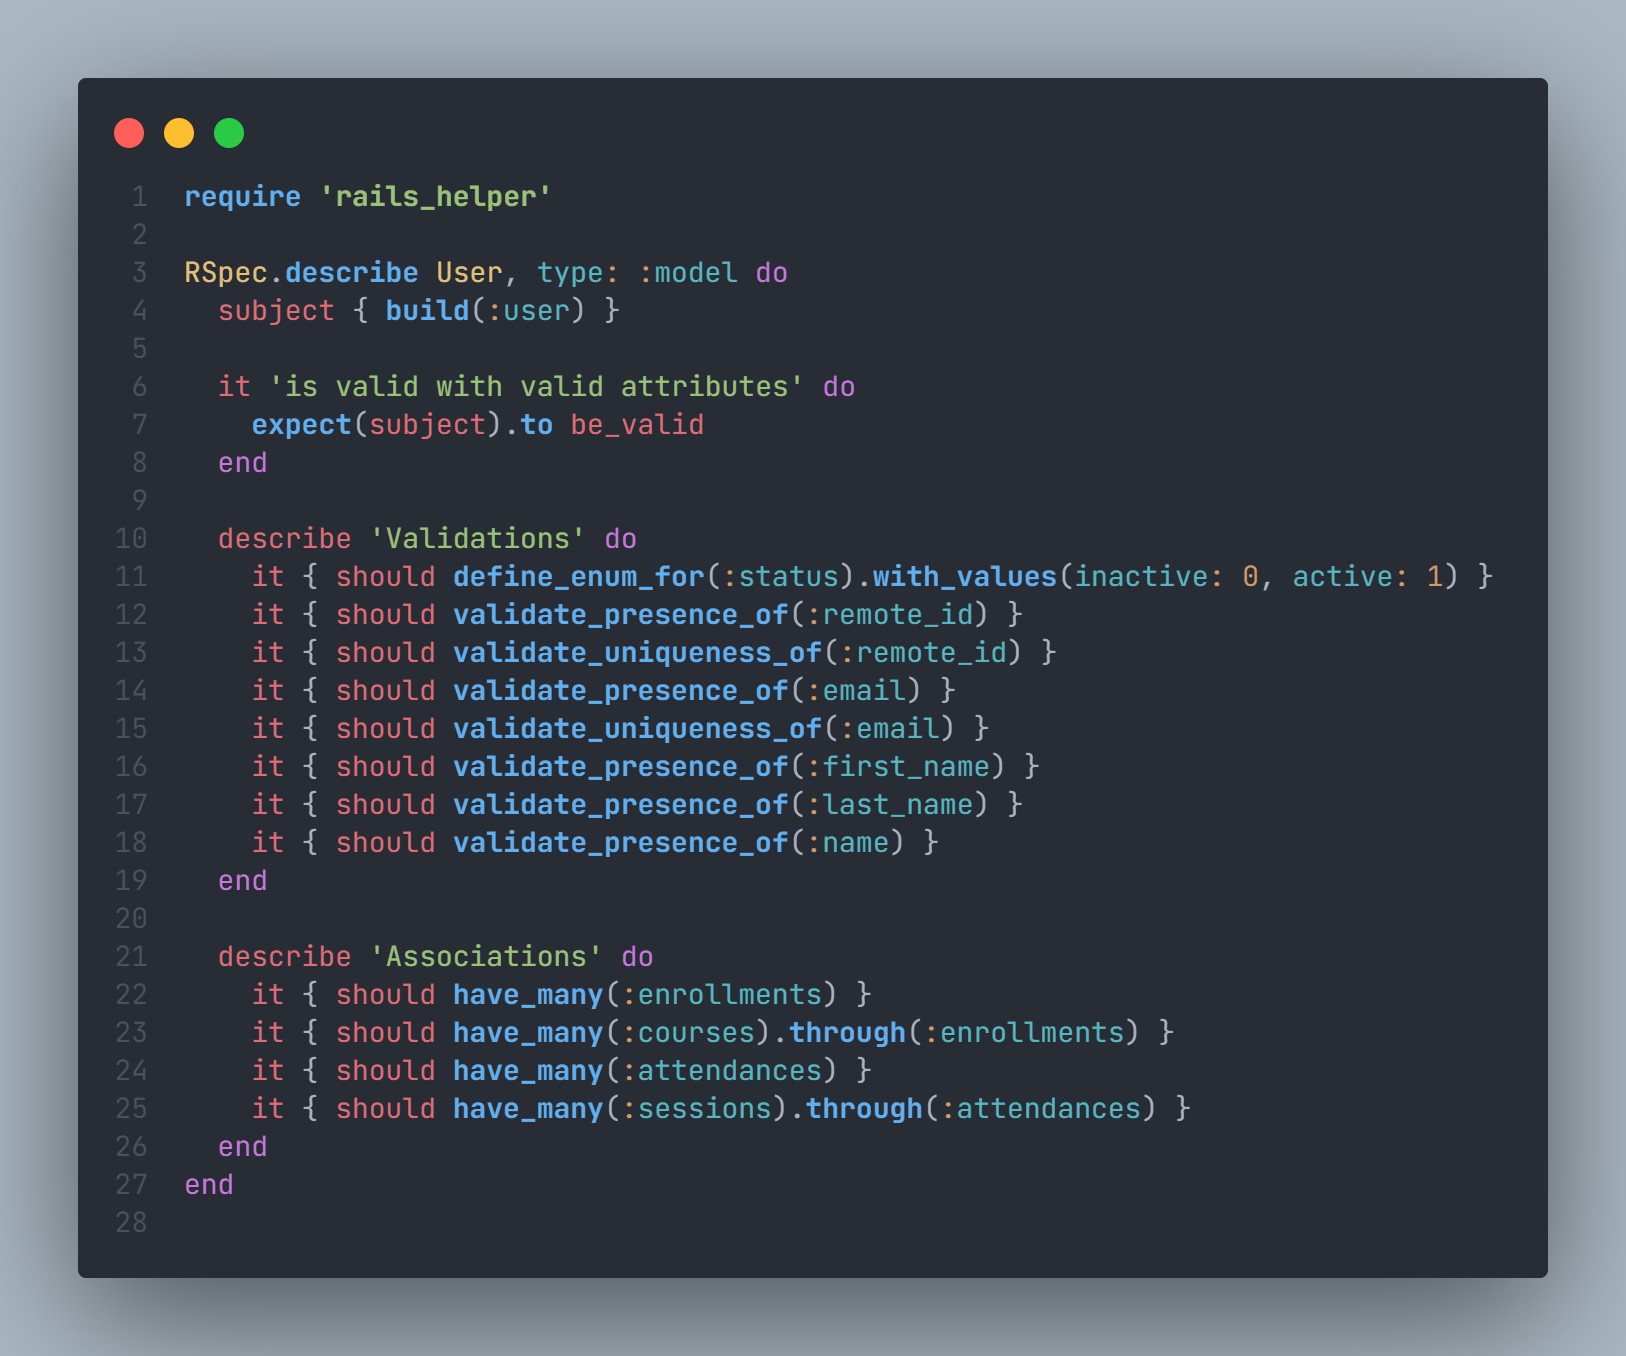
\includegraphics[width=140mm,scale=1]{figures/implementation_and_testing/testing/AUT/user/all.png}}
        \caption{User Model Unit Tests}
        \label{User Model Unit Tests}
    \end{figure}


%%%%%%%%%%%%%%%%%%%%%%%%%%%%%%%%%%%%%%%%%%%%%%%%%%%%%%%%%%%%%%%%%
%%%%%%%%%%%%%%%%%%%%%%%%%%%%%%%%%%%%%%%%%%%%%%%%%%%%%%%%%%%%%%%%%


\newendline \textbf{\textit{Session Model}}\newendline
The unit tests that have been completed for the Session model are as follows.

\vspace{0.25cm}
\newendline
\textbf{Attribute Validations}

    \begin{figure}[H]
        \centerline{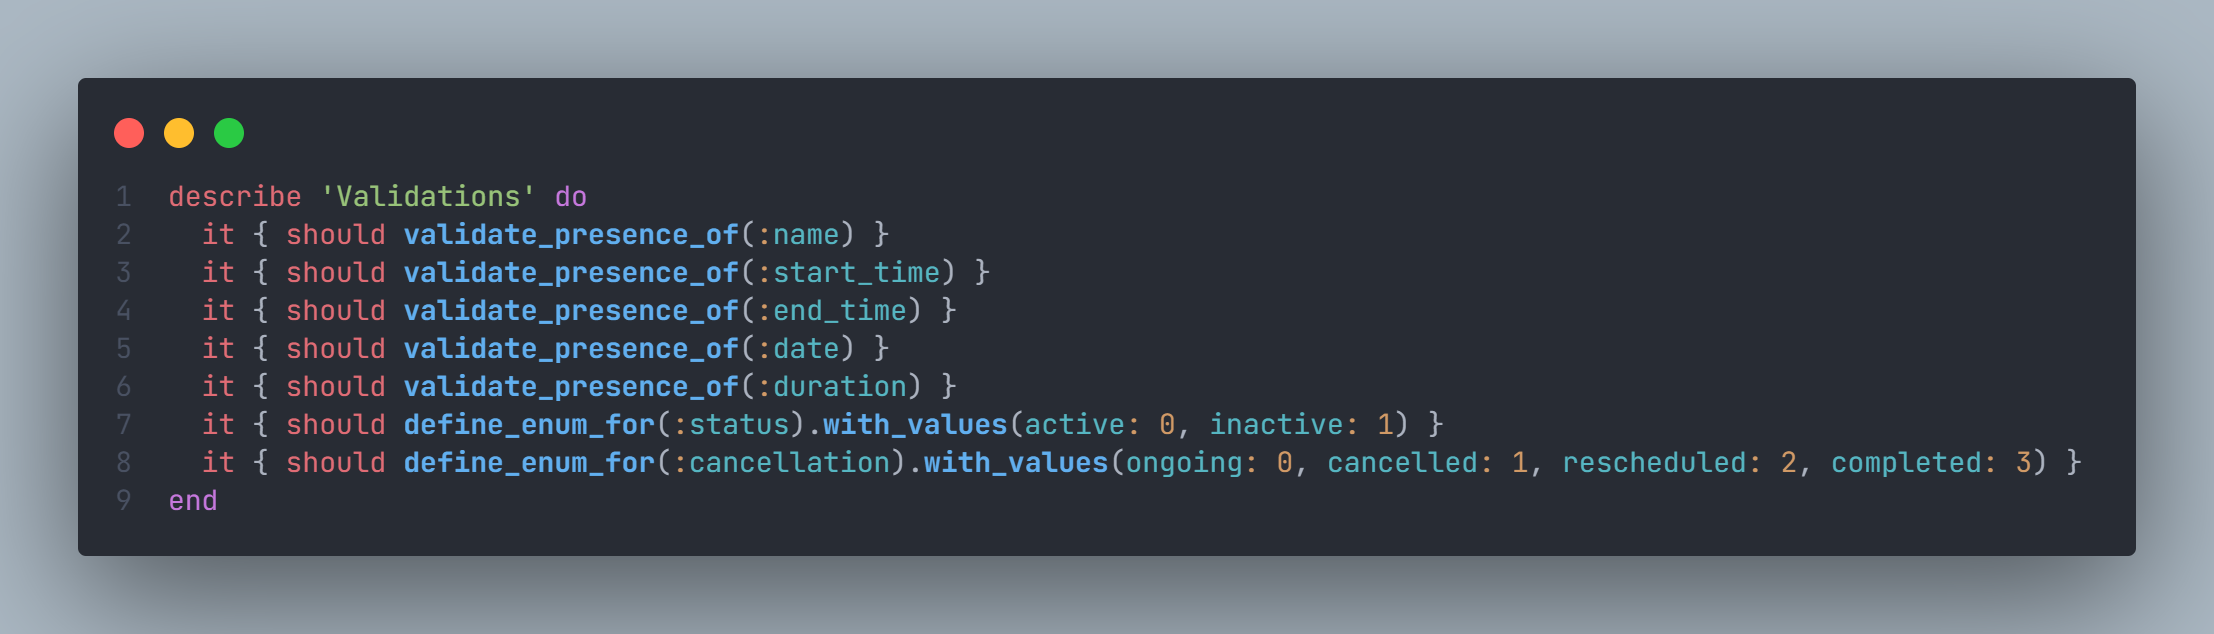
\includegraphics[width=140mm,scale=1]{figures/implementation_and_testing/testing/AUT/session/validations.png}}
        \caption{Session Model - Validation Unit Tests}
        \label{Session Model - Validation Unit Tests}
    \end{figure}

\vspace{0.25cm}
\noindent\textbf{\textit{\underline{Presence validation:}}} The validate\_presence\_of tests are used to ensure that a Session instance cannot be saved without certain critical attributes. This is demonstrated in our suite by tests such as validate\_presence\_of(:name), validate\_presence\_of(:st- art\_time), validate\_presence\_of(:end\_time), validate\_presence\_of(:date), and validate\_presence\_of(:duration), which ensure that each session must have these key attributes.

\vspace{0.25cm}
\noindent\textbf{\textit{\underline{Enumeration validation:}}} We use define\_enum\_for to validate that named values of an attribute accurately correspond to integer values in the database. In our suite, define\_enum\_for(:status).with\_values(active: 0, inactive: 1) verifies the status attribute maps 'active' and 'inactive' to 0 and 1, respectively. define\_enum\_for(:cancellation)- .with\_values(ongoing: 0, cancelled: 1, rescheduled: 2, completed: 3) ensures that the 'cancellation' attribute maps 'ongoing', 'cancelled', 'rescheduled', and 'completed' to 0, 1, 2, and 3, respectively.

\vspace{0.25cm}
\newendline
\textbf{Model Associations}

    \begin{figure}[H]
        \centerline{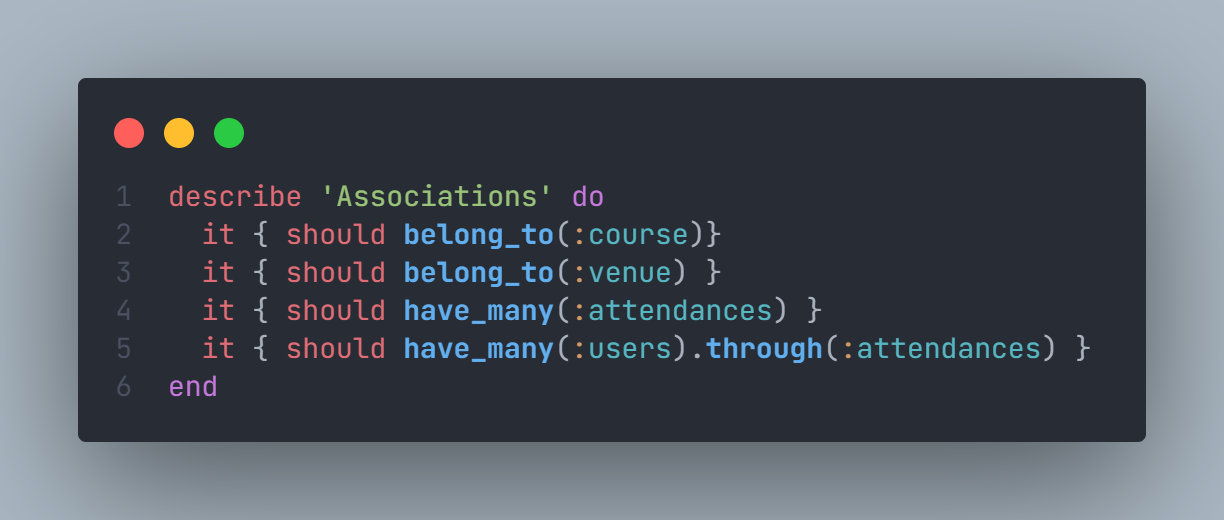
\includegraphics[width=140mm,scale=1]{figures/implementation_and_testing/testing/AUT/session/associations.png}}
        \caption{Session Model - Association Unit Tests}
        \label{Session Model - Association Unit Tests}
    \end{figure}

\vspace{0.25cm}
\noindent\textbf{\textit{\underline{One-to-one relationships:}}} The belong\_to test checks the presence of one-to-one associations between models. In our suite, it { should belong\_to(:course)} and it { should belong\_to(:venue) } validate that each session belongs to a single course and a single venue.\\

\vspace{0.25cm}
\noindent\textbf{\textit{\underline{One-to-many relationships:}}} The have\_many test validates that one instance of the Session model can be associated with multiple instances of another model. For instance, it { should have\_many(:attendances) } asserts that a Session can have multiple Attendances.

\vspace{0.25cm}
\noindent\textbf{\textit{\underline{Many-to-many relationships:}}} The have\_many...through test is used when a Session instance can be associated with many instances of another model via a third model. it { should have\_many(:users).through(:attendances) } in our test suite validates that a Session can be associated with many Users through Attendances.


    \begin{figure}[H]
        \centerline{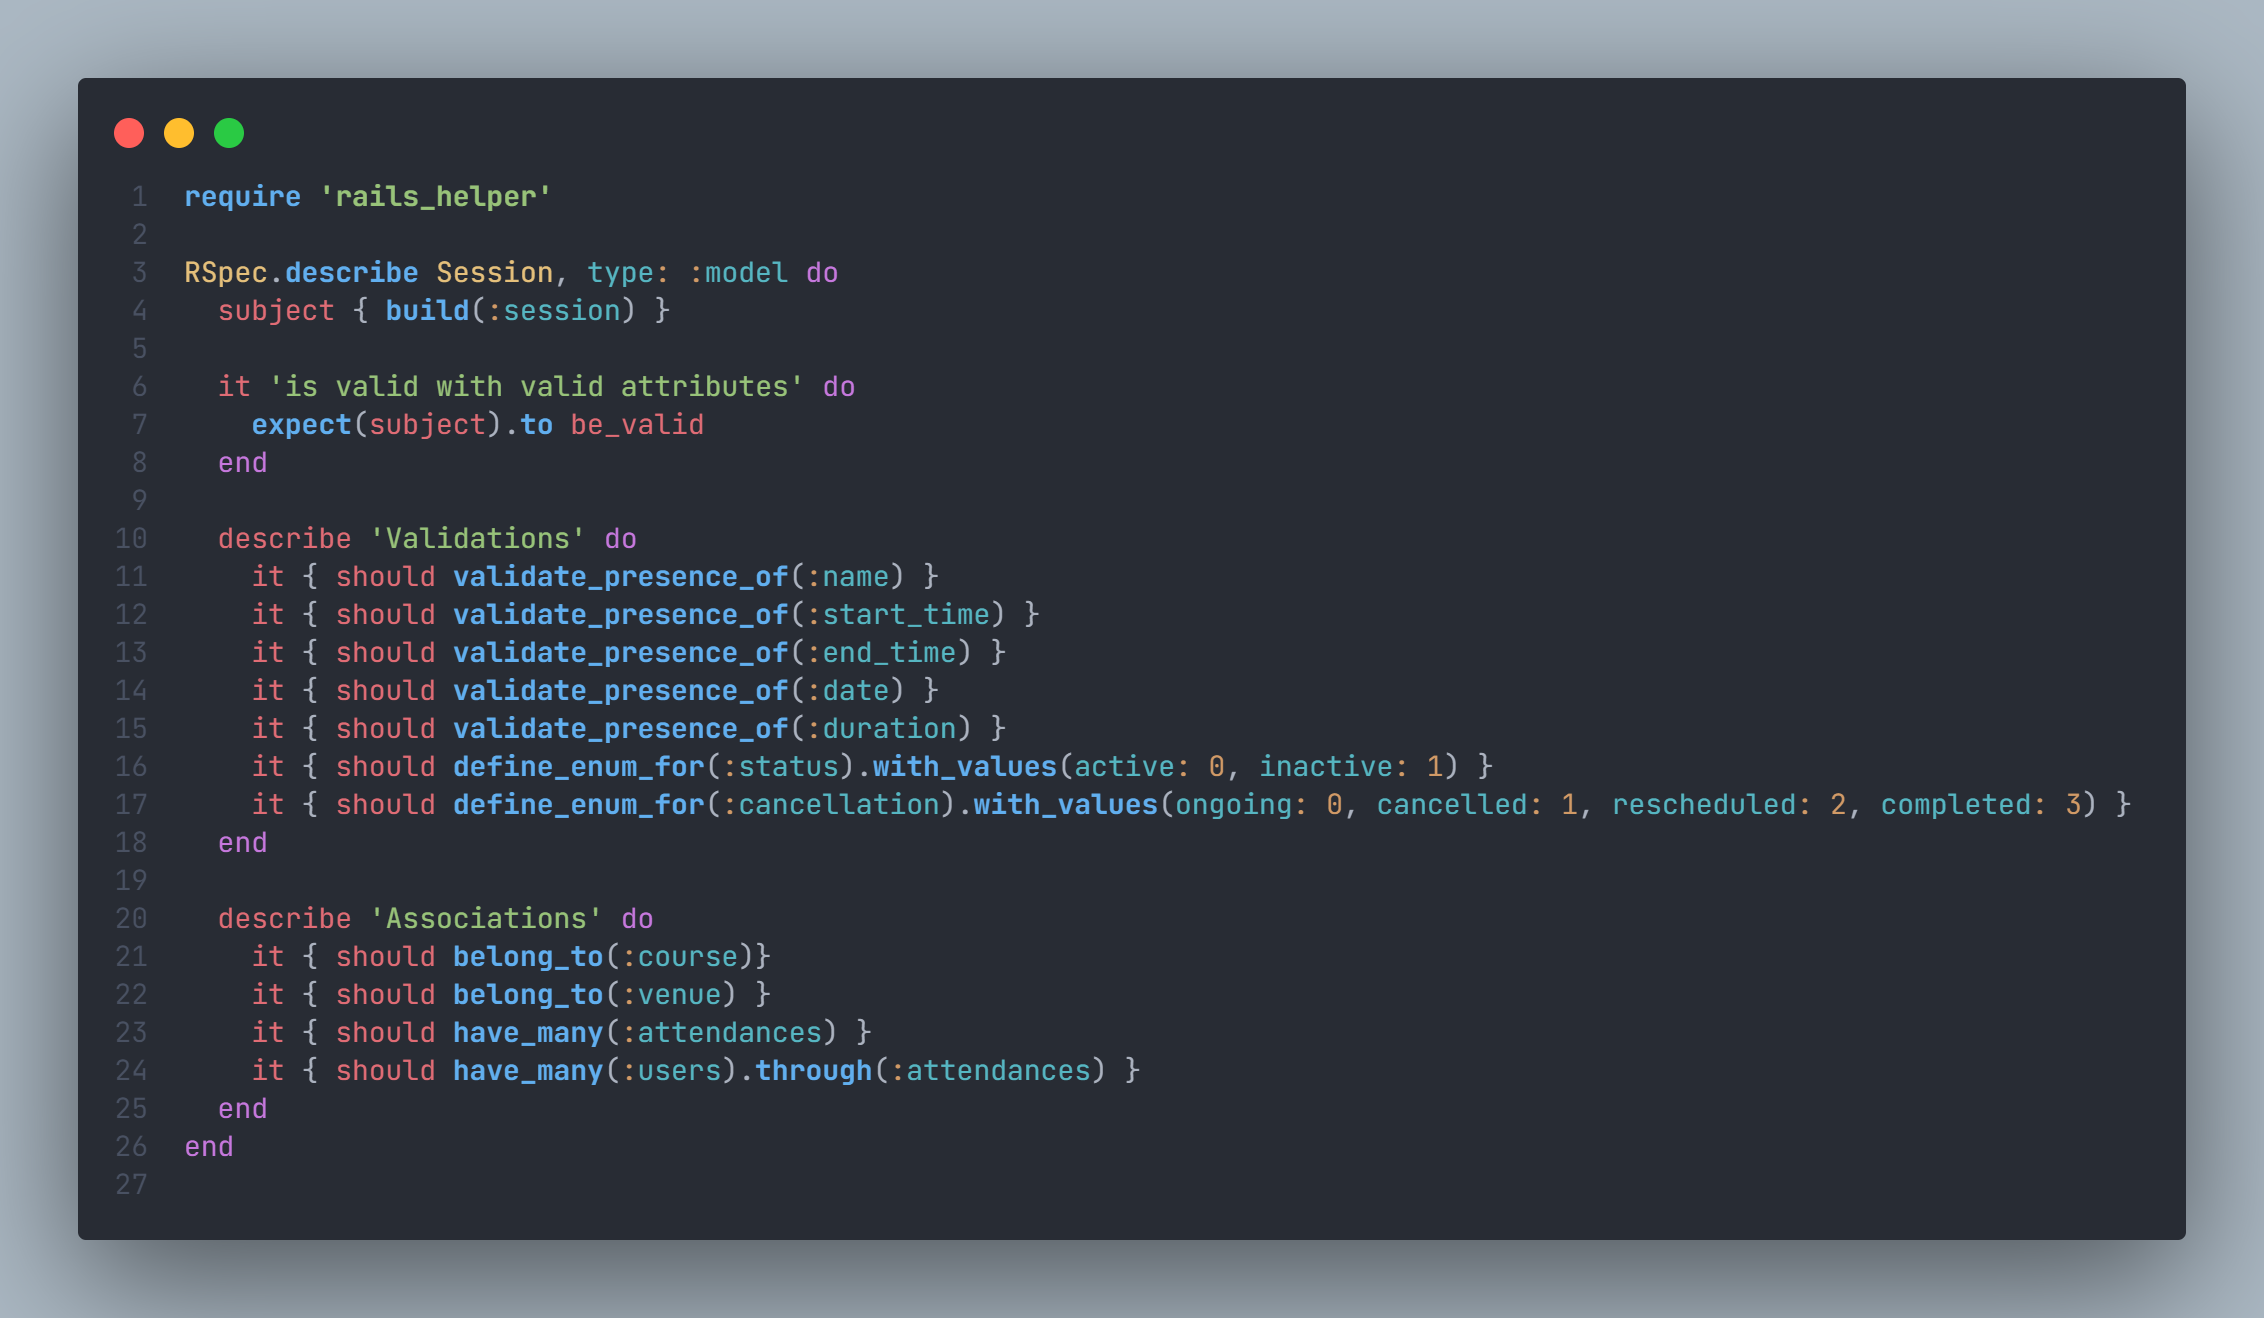
\includegraphics[width=140mm,scale=1]{figures/implementation_and_testing/testing/AUT/session/all.png}}
        \caption{Session Model Unit Tests}
        \label{Session Model Unit Tests}
    \end{figure}



%%%%%%%%%%%%%%%%%%%%%%%%%%%%%%%%%%%%%%%%%%%%%%%%%%%%%%%%%%%%%%%%%
%%%%%%%%%%%%%%%%%%%%%%%%%%%%%%%%%%%%%%%%%%%%%%%%%%%%%%%%%%%%%%%%%


\newendline \textbf{\textit{Venue Model}}\newendline
The unit tests that have been completed for the Venue model are as follows.

\vspace{0.25cm}
\newendline
\textbf{Attribute Validations}

    \begin{figure}[H]
        \centerline{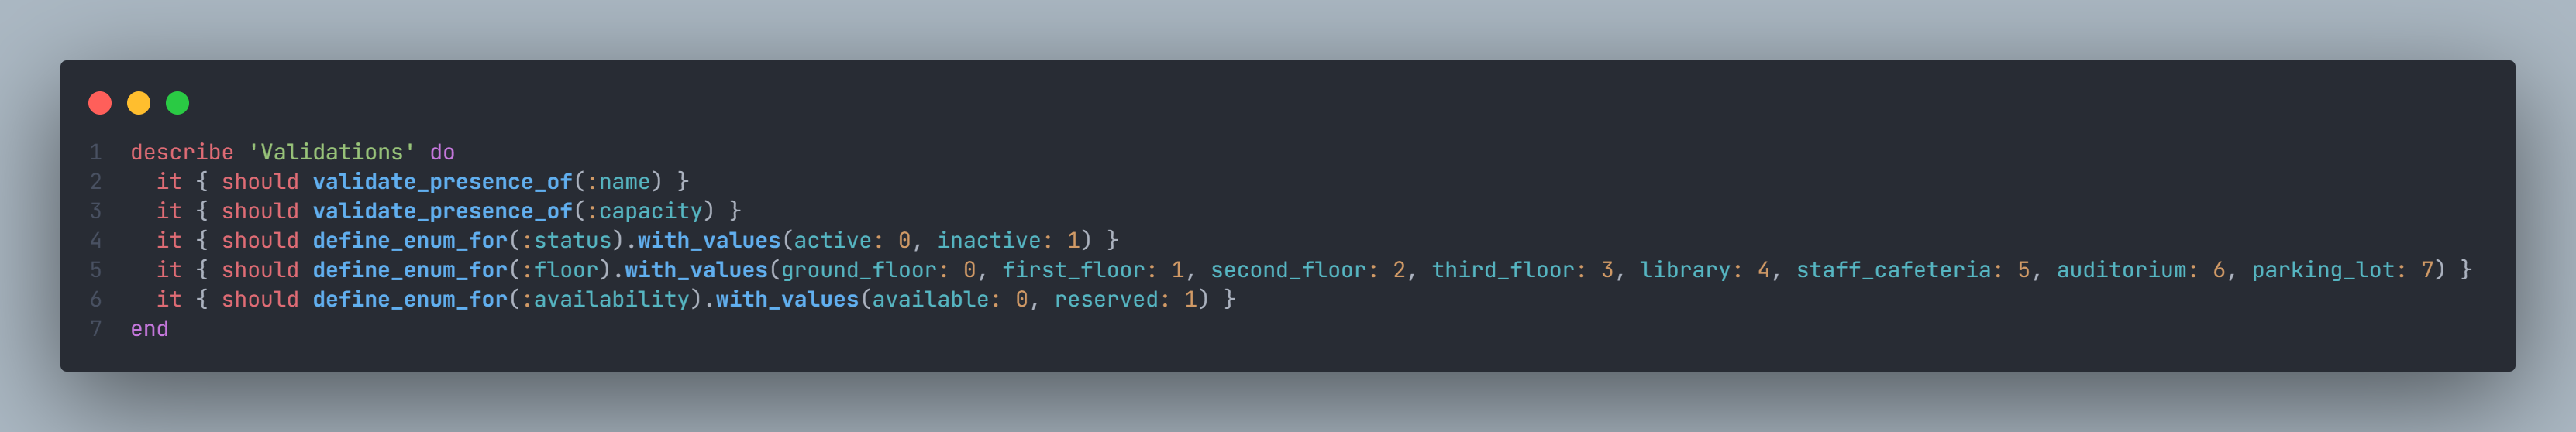
\includegraphics[width=150mm,scale=1]{figures/implementation_and_testing/testing/AUT/venue/validations.png}}
        \caption{Venue Model - Validation Unit Tests}
        \label{Venue Model - Validation Unit Tests}
    \end{figure}

\vspace{0.25cm}
\noindent\textbf{\textit{\underline{Presence validation:}}} The validate\_presence\_of tests are designed to confirm that a Venue instance cannot be saved without certain vital attributes. This is depicted in our suite by tests such as validate\_presence\_of(:name) and validate\_presence\_of(- :c-apacity), which guarantee that each venue must have a name and a capacity.

\vspace{0.25cm}
\noindent\textbf{\textit{\underline{Enumeration validation:}}} define\_enum\_for is used to ensure that named values of an attribute accurately correspond to integer values in the database. In our suite, define\_enum\_for(:status).with\_values(active: 0, inactive: 1) ensures that the status attribute correctly maps 'active' and 'inactive' to 0 and 1, respectively. define\_enum\_- for(:floor).with\_values(ground\_floor: 0, first\_floor: 1, second\_floor: 2, third\_floor: 3, library: 4, staff\_cafeteria: 5, auditorium: 6, parking\_lot: 7) confirms that the 'floor' attribute maps correctly to these respective integer values. Moreover, define\_enum\_for(:availability).with\_values(available: 0, reserved: 1) verifies that the availability attribute accurately maps 'available' and 'reserved' to 0 and 1, respectively.

\vspace{0.25cm}
\newendline
\textbf{Model Associations}

    \begin{figure}[H]
        \centerline{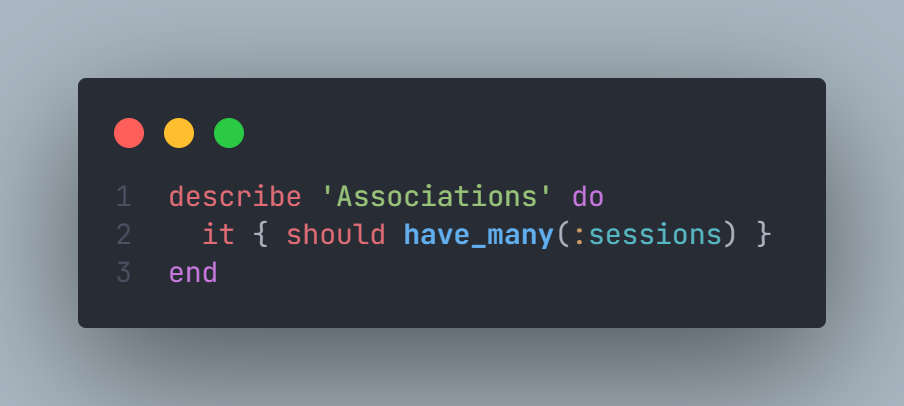
\includegraphics[width=140mm,scale=1]{figures/implementation_and_testing/testing/AUT/venue/associations.png}}
        \caption{Venue Model - Association Unit Tests}
        \label{Venue Model - Association Unit Tests}
    \end{figure}

\vspace{0.25cm}
\noindent\textbf{\textit{\underline{One-to-many relationships:}}} The have\_many test confirms the presence of one-to-many associations between models. In our suite, it { should have\_many(:sessions) } validates that a Venue can host multiple Sessions.


    \begin{figure}[H]
        \centerline{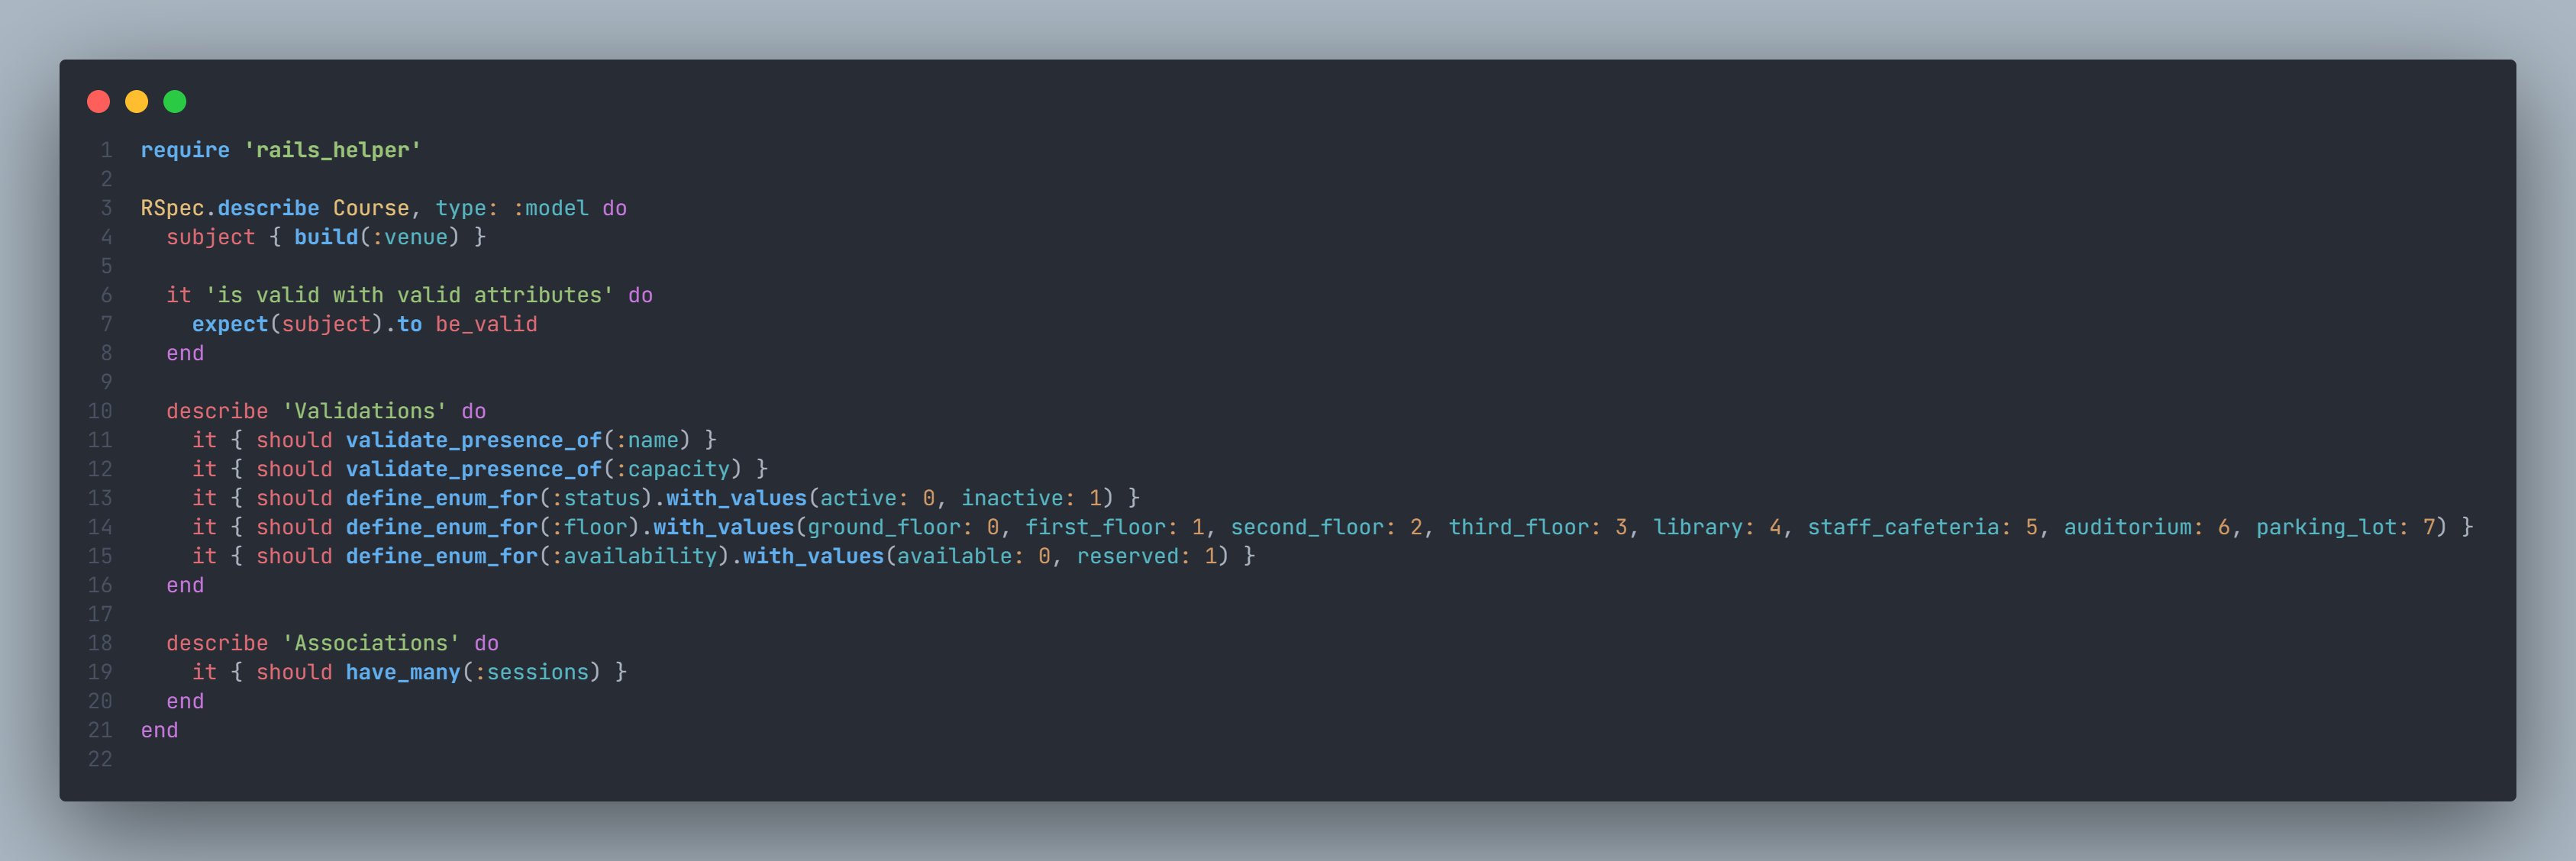
\includegraphics[width=140mm,scale=1]{figures/implementation_and_testing/testing/AUT/venue/all.png}}
        \caption{Venue Model Unit Tests}
        \label{Venue Model Unit Tests}
    \end{figure}



%%%%%%%%%%%%%%%%%%%%%%%%%%%%%%%%%%%%%%%%%%%%%%%%%%%%%%%%%%%%%%%%%
%%%%%%%%%%%%%%%%%%%%%%%%%%%%%%%%%%%%%%%%%%%%%%%%%%%%%%%%%%%%%%%%%


\newendline \textbf{\textit{Question Model}}\newendline
The unit tests that have been completed for the Question model are as follows.

\vspace{0.25cm}
\newendline
\textbf{Attribute Validations}

    \begin{figure}[H]
        \centerline{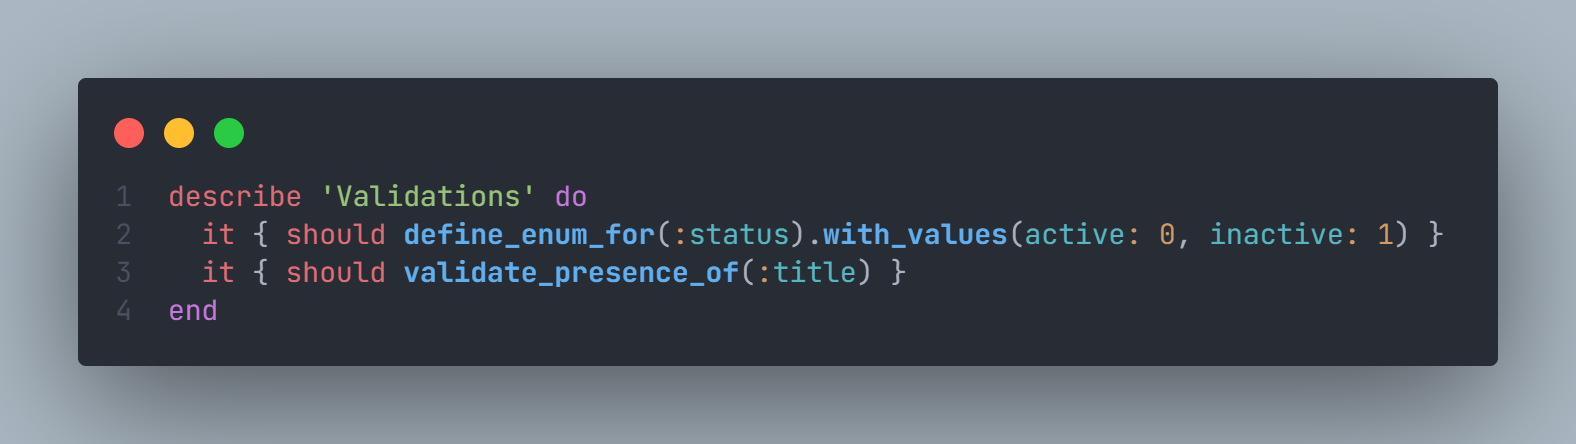
\includegraphics[width=140mm,scale=1]{figures/implementation_and_testing/testing/AUT/question/validations.png}}
        \caption{Question Model - Validation Unit Tests}
        \label{Question Model - Validation Unit Tests}
    \end{figure}

\vspace{0.25cm}
\noindent\textbf{\textit{\underline{Presence validation:}}} The validate\_presence\_of test is applied to make sure a Question instance cannot be saved without essential attributes. This is shown in our test suite by validate\_presence\_of(:title), ensuring each question must have a title.

\vspace{0.25cm}
\noindent\textbf{\textit{\underline{Enumeration validation:}}} The define\_enum\_for method is used for validating that the named values of an attribute correctly map to integer values in the database. In our suite, define\_enum\_for(:status).with\_values(active: 0, inactive: 1) verifies the status attribute accurately maps 'active' and 'inactive' to 0 and 1, respectively.

\clearpage
\vspace{0.25cm}
\newendline
\textbf{Model Associations}

    \begin{figure}[H]
        \centerline{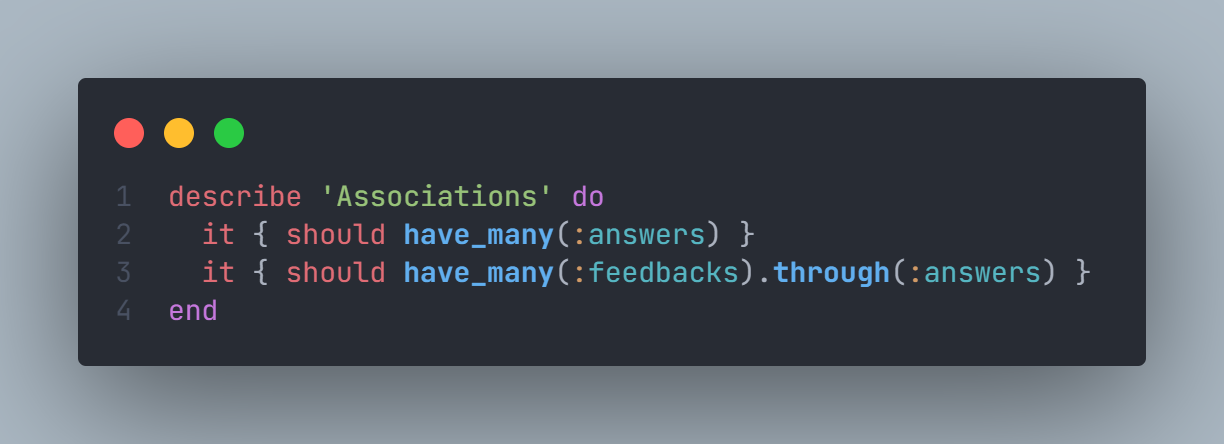
\includegraphics[width=140mm,scale=1]{figures/implementation_and_testing/testing/AUT/question/associations.png}}
        \caption{Question Model - Association Unit Tests}
        \label{Question Model - Association Unit Tests}
    \end{figure}

\vspace{0.25cm}
\noindent\textbf{\textit{\underline{One-to-many relationships:}}} The have\_many test verifies that one instance of the Question model can be associated with multiple instances of another model. In our test suite, it { should have\_many(:answers) } confirms that a Question can have multiple Answers.

\vspace{0.25cm}
\noindent\textbf{\textit{\underline{Many-to-many relationships:}}} The have\_many...through test is employed when a Question instance can be associated with many instances of another model via a third model. In our test suite, it { should have\_many(:feedbacks).through(:answers) } validates that a Question can be associated with many Feedbacks through Answers.

    \begin{figure}[H]
        \centerline{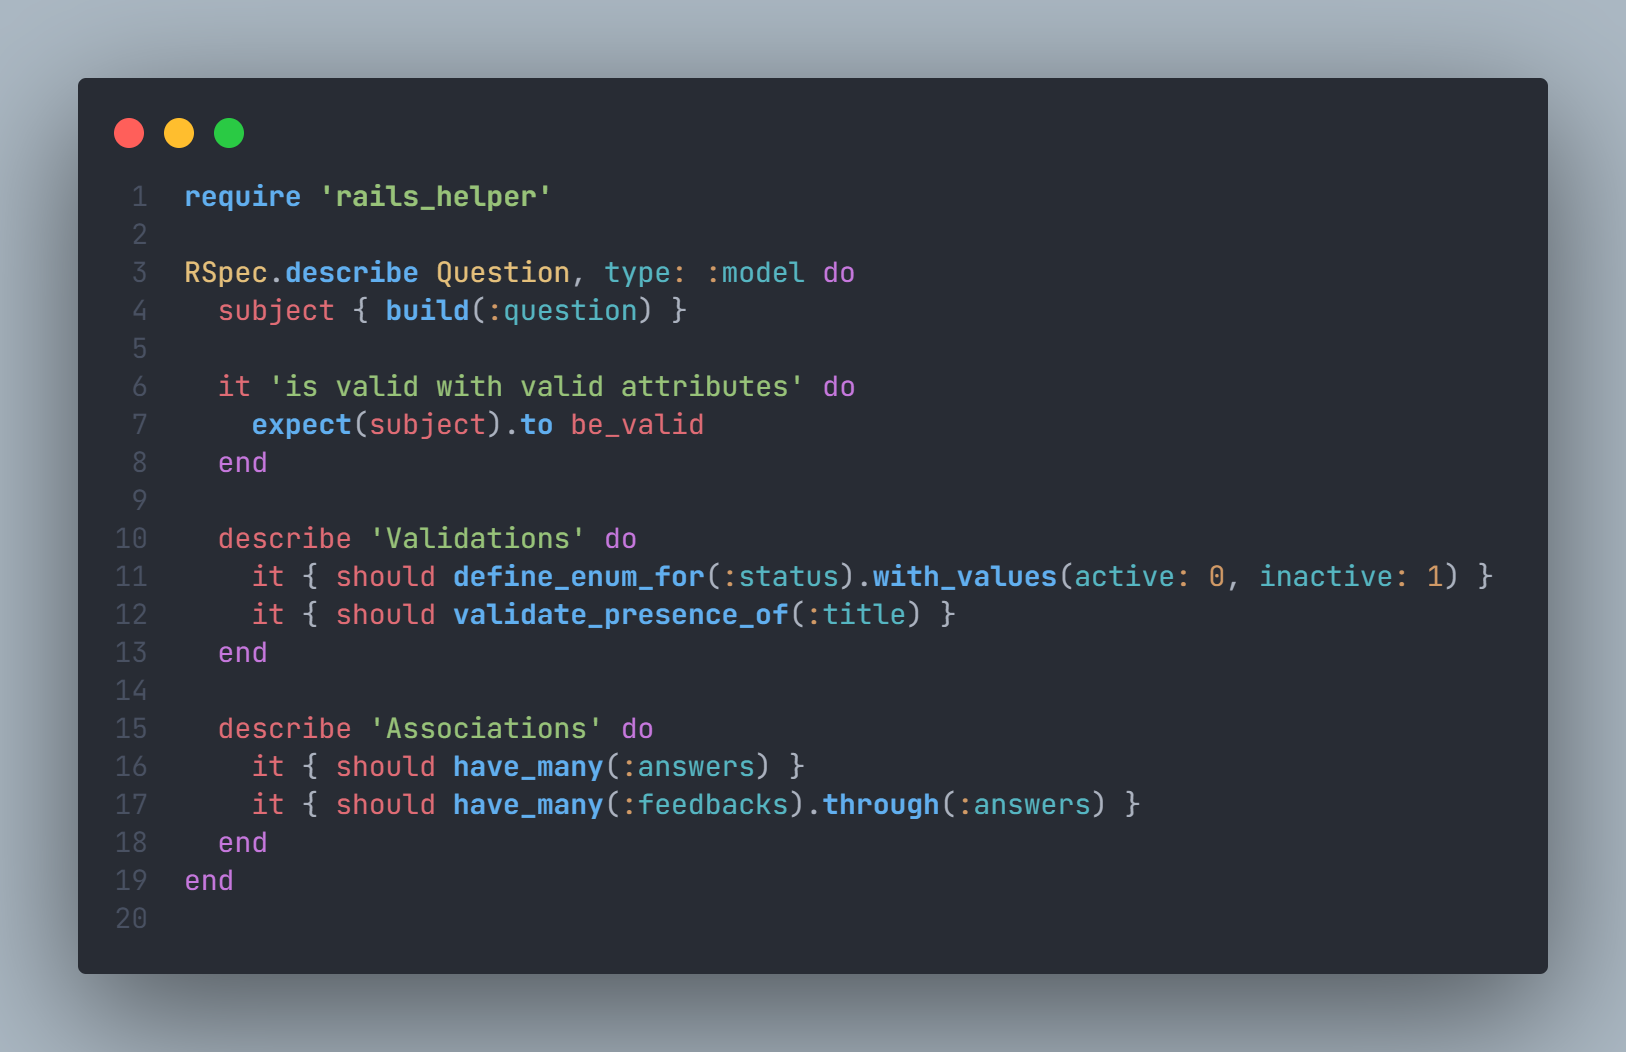
\includegraphics[width=130mm,scale=1]{figures/implementation_and_testing/testing/AUT/question/all.png}}
        \caption{Question Model Unit Tests}
        \label{Question Model Unit Tests}
    \end{figure}

%%%%%%%%%%%%%%%%%%%%%%%%%%%%%%%%%%%%%%%%%%%%%%%%%%%%%%%%%%%%%%%%%
%%%%%%%%%%%%%%%%%%%%%%%%%%%%%%%%%%%%%%%%%%%%%%%%%%%%%%%%%%%%%%%%%


\newendline \textbf{\textit{Feedback Model}}\newendline
The unit tests that have been completed for the Feedback model are as follows.

\vspace{0.25cm}
\newendline
\textbf{Attribute Validations}

    \begin{figure}[H]
        \centerline{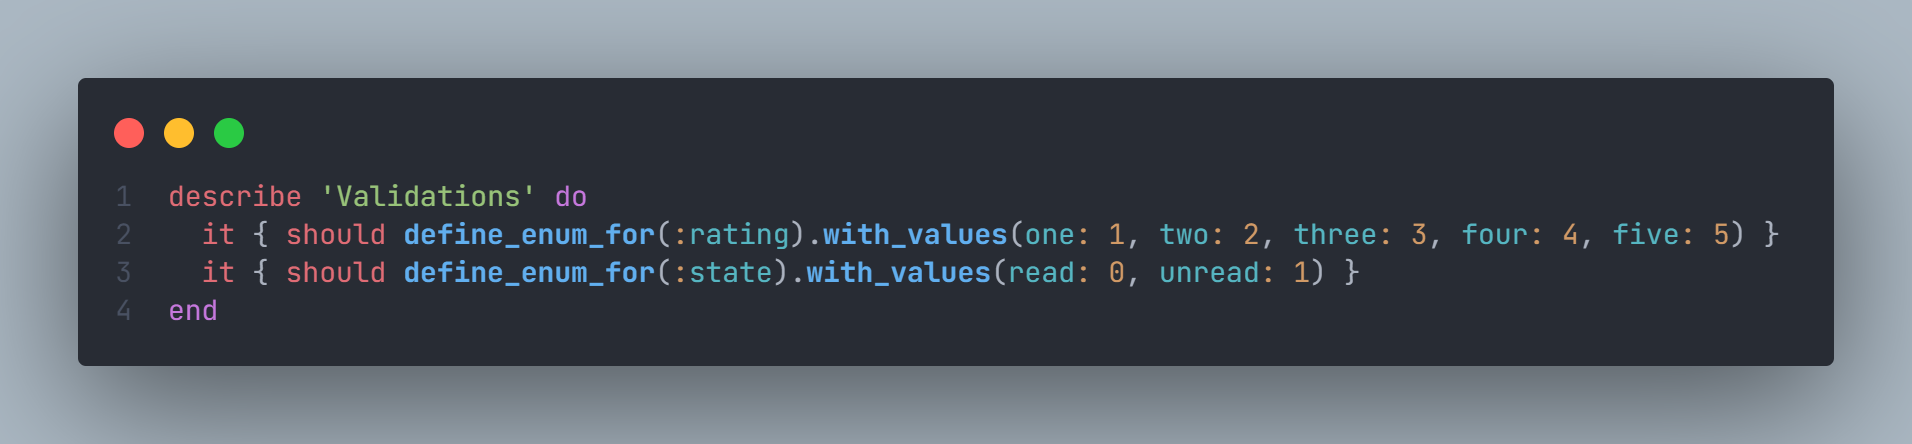
\includegraphics[width=140mm,scale=1]{figures/implementation_and_testing/testing/AUT/feedback/validations.png}}
        \caption{Feedback Model - Validation Unit Tests}
        \label{Feedback Model - Validation Unit Tests}
    \end{figure}

\vspace{0.25cm}
\noindent\textbf{\textit{\underline{Enumeration validation:}}} The define\_enum\_for method is employed for validating the mapping of named values of an attribute to integer values in the database. In our suite, define\_enum\_for(:rating).with\_values(one: 1, two: 2, three: 3, four: 4, five: 5) ensures the rating attribute correctly maps the terms 'one' through 'five' to 1 through 5, respectively. Similarly, define\_enum\_for(:state).with\_values(read: 0, unread: 1) verifies the state attribute accurately maps 'read' and 'unread' to 0 and 1, respectively.

\vspace{0.25cm}
\newendline
\textbf{Model Associations}

    \begin{figure}[H]
        \centerline{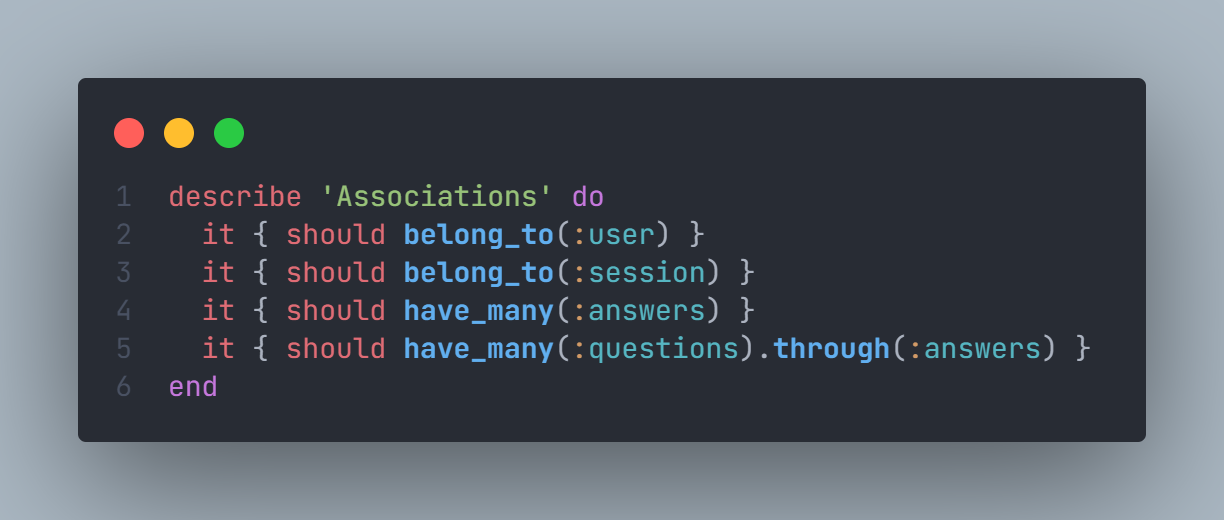
\includegraphics[width=140mm,scale=1]{figures/implementation_and_testing/testing/AUT/feedback/associations.png}}
        \caption{Feedback Model - Association Unit Tests}
        \label{Feedback Model - Association Unit Tests}
    \end{figure}

\clearpage
\vspace{0.25cm}
\noindent\textbf{\textit{\underline{One-to-one relationships:}}} The belong\_to test validates that an instance of the Feedback model can be associated with one instance of another model. In our test suite, it { should belong\_to(:user) } and it { should belong\_to(:session) } confirm that a Feedback instance can be related to a specific User and Session.

\vspace{0.25cm}
\noindent\textbf{\textit{\underline{One-to-many relationships:}}} The have\_many test confirms that one instance of the Feedback model can be associated with multiple instances of another model. In our suite, it { should have\_many(:answers) } verifies that a Feedback can have multiple Answers.

\vspace{0.25cm}
\noindent\textbf{\textit{\underline{Many-to-many relationships:}}} The have\_many...through test is used when a Feedback instance can be associated with many instances of another model via a third model. In our suite, it { should have\_many(:questions).through(:answers) } validates that a Feedback can be associated with many Questions through Answers.

    \begin{figure}[H]
        \centerline{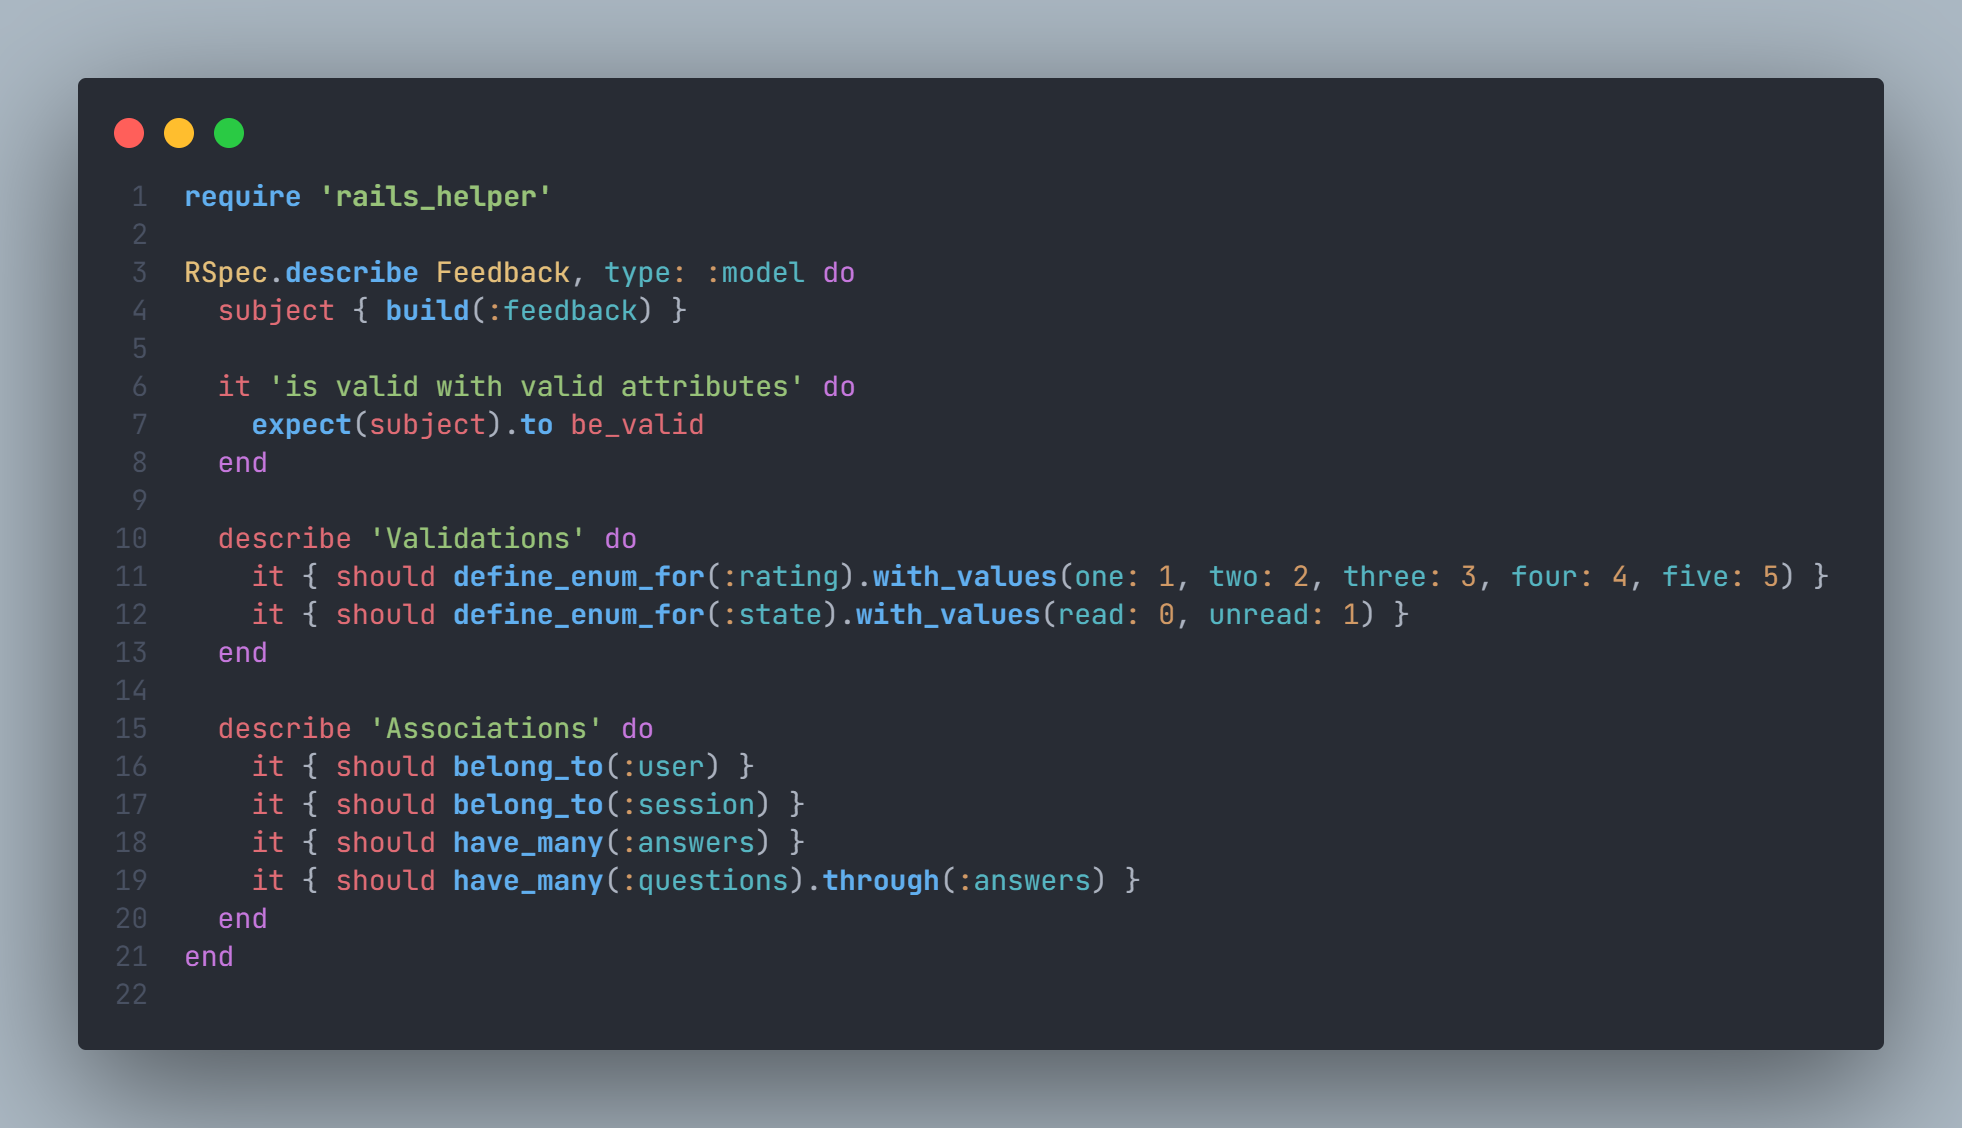
\includegraphics[width=140mm,scale=1]{figures/implementation_and_testing/testing/AUT/feedback/all.png}}
        \caption{Feedback Model Unit Tests}
        \label{Feedback Model Unit Tests}
    \end{figure}

%%%%%%%%%%%%%%%%%%%%%%%%%%%%%%%%%%%%%%%%%%%%%%%%%%%%%%%%%%%%%%%%%
%%%%%%%%%%%%%%%%%%%%%%%%%%%%%%%%%%%%%%%%%%%%%%%%%%%%%%%%%%%%%%%%%


\clearpage
\newendline \textbf{\textit{Material Model}}\newendline
The unit tests that have been completed for the Material model are as follows.

\vspace{0.25cm}
\newendline
\textbf{Attribute Validations}


    \begin{figure}[H]
        \centerline{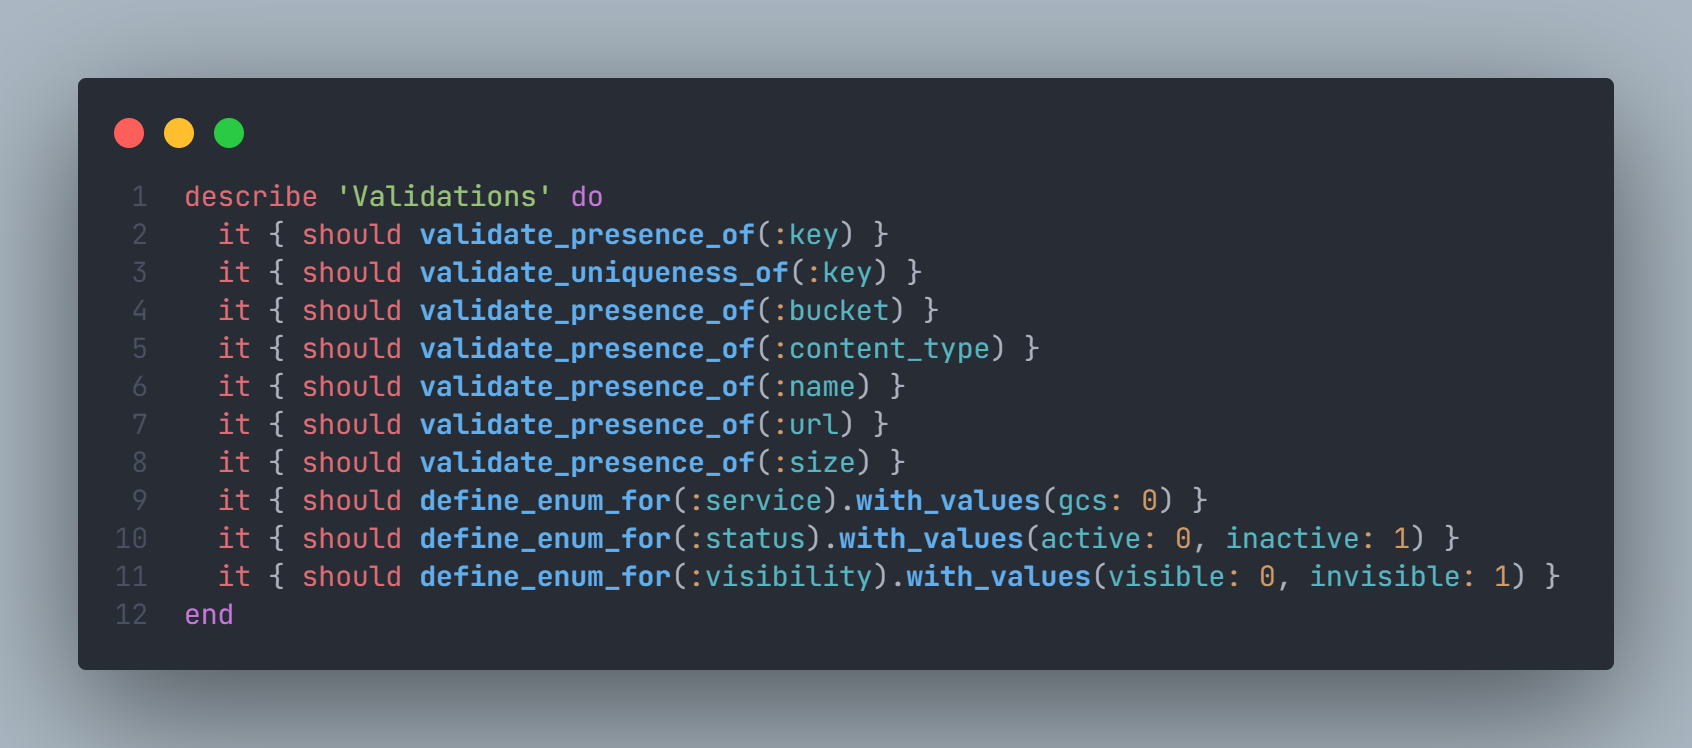
\includegraphics[width=140mm,scale=1]{figures/implementation_and_testing/testing/AUT/material/validations.png}}
        \caption{Material Model - Validation Unit Tests}
        \label{Material Model - Validation Unit Tests}
    \end{figure}

\vspace{0.25cm}
\noindent\textbf{\textit{\underline{Presence validation:}}} The validate\_presence\_of tests ensure that certain attributes must contain values. For example, validate\_presence\_of(:name), validate\_presence- \_of(:url), validate\_presence\_of(:size), etc., verifies that a Material instance cannot be saved without these respective attributes.

\vspace{0.25cm}
\noindent\textbf{\textit{\underline{Uniqueness validation:}}} These tests validate that the value of certain attributes is unique across all instances of a model, ensuring that no two materials can share the same value of such an attribute. For instance, validate\_uniqueness\_of(:key) asserts that each Material has a unique key.

\vspace{0.25cm}
\noindent\textbf{\textit{\underline{Enumeration validation:}}} We use define\_enum\_for to validate enumerations, where a set of named values correspond to integer values in the database. For example, define\_enum\_for(:service).with\_values(gcs: 0), define\_enum\_for(:status).with\_val- ues(active: 0, inactive: 1), and define\_enum\_for(:visibility).with\_values(visible: 0, invisible: 1) confirm that the service, status, and visibility attributes accurately map the respective terms to 0 and 1.\\

\vspace{0.25cm}
\newendline
\textbf{Model Associations}

    \begin{figure}[H]
        \centerline{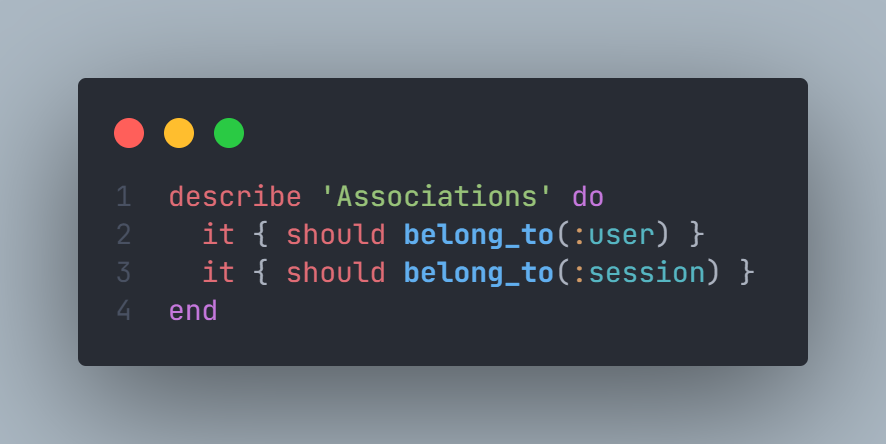
\includegraphics[width=140mm,scale=1]{figures/implementation_and_testing/testing/AUT/material/associations.png}}
        \caption{Material Model - Association Unit Tests}
        \label{Material Model - Association Unit Tests}
    \end{figure}


\vspace{-0.5cm}
\noindent\textbf{\textit{\underline{One-to-one relationships:}}} The belong\_to test validates that an instance of the Material model can be associated with one instance of another model. In our test suite, it { should belong\_to(:user) } and it { should belong\_to(:session) } confirm that a Material instance can be associated with a specific User and Session.


    \begin{figure}[H]
        \centerline{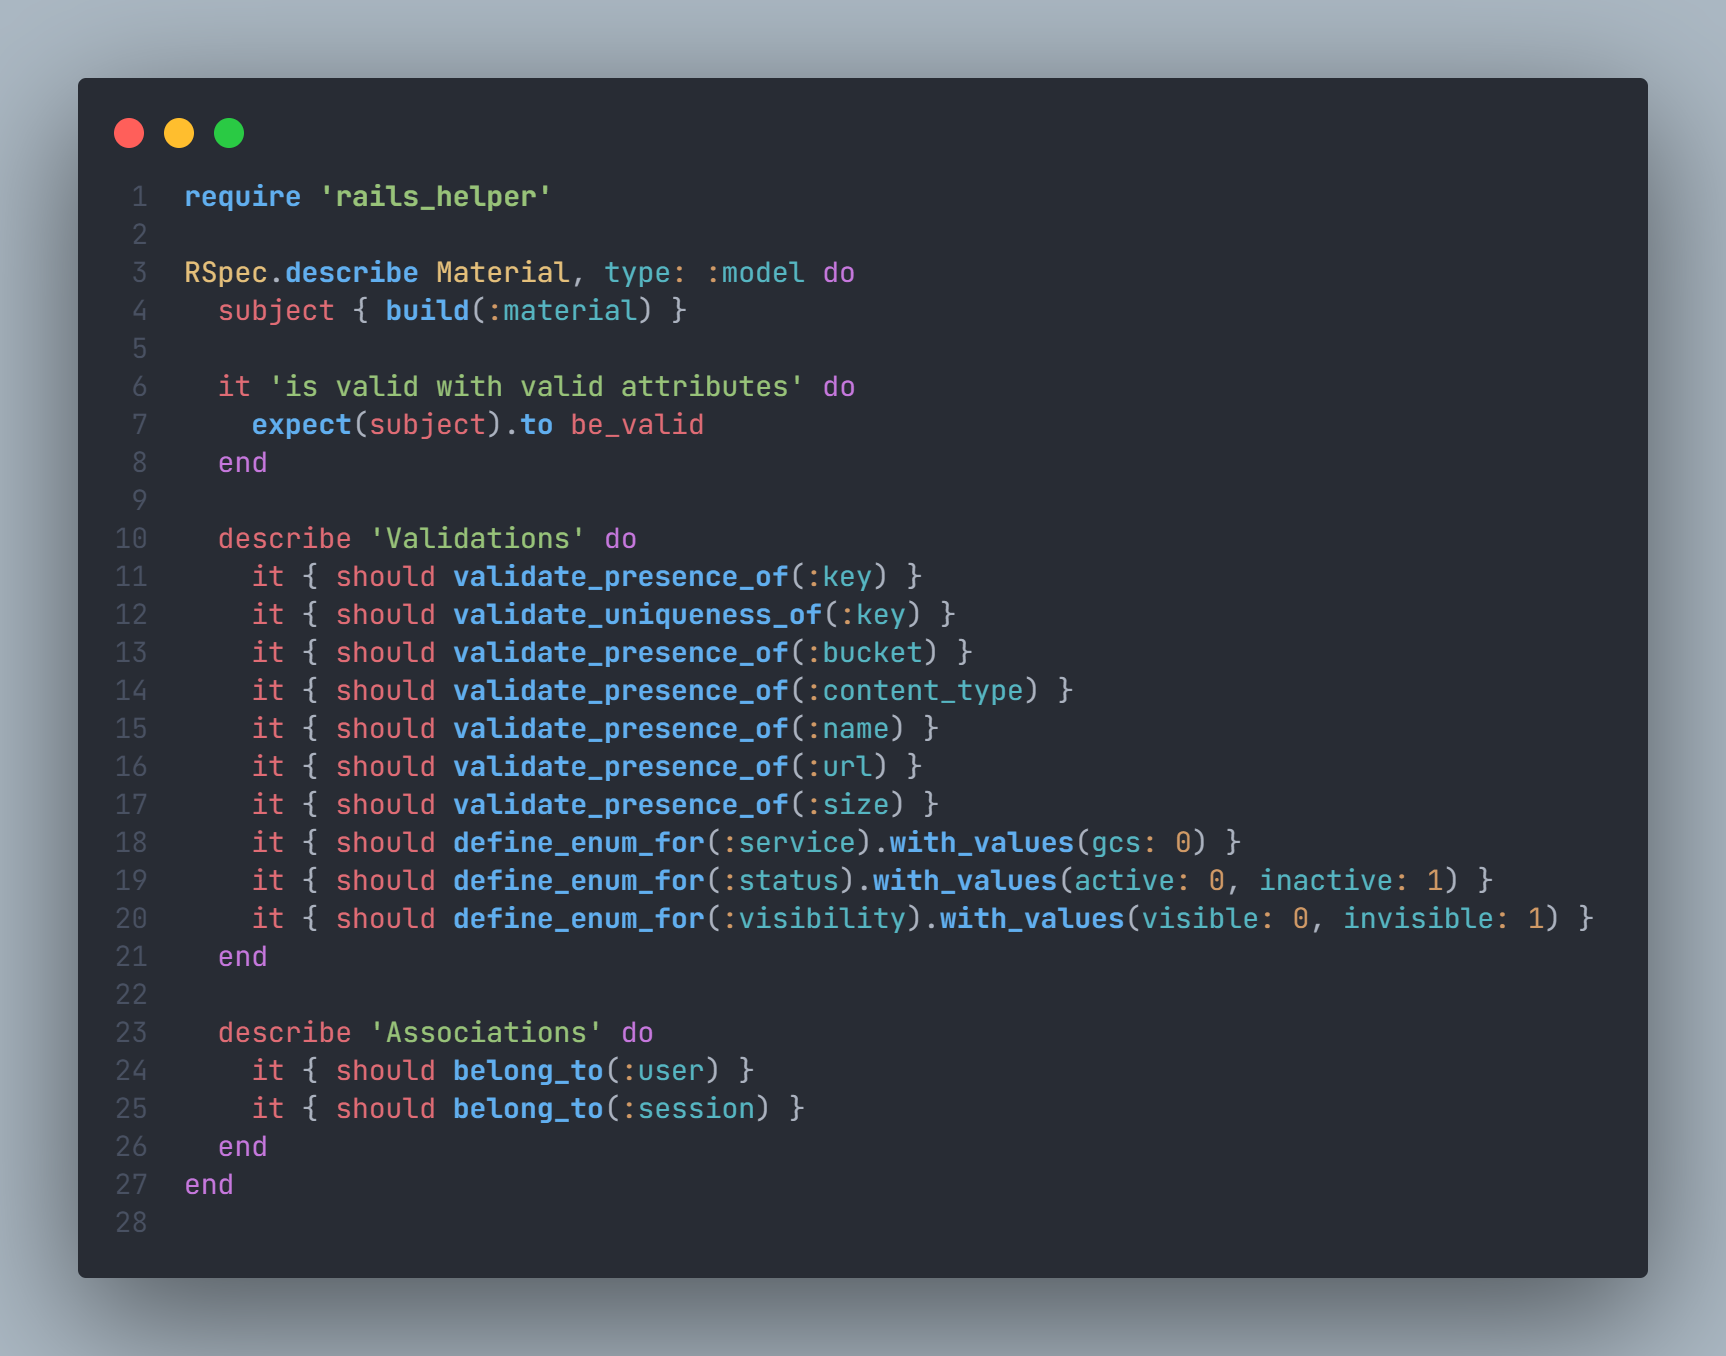
\includegraphics[width=140mm,scale=1]{figures/implementation_and_testing/testing/AUT/material/all.png}}
        \caption{Material Model Unit Tests}
        \label{Material Model Unit Tests}
    \end{figure}



%%%%%%%%%%%%%%%%%%%%%%%%%%%%%%%%%%%%%%%%%%%%%%%%%%%%%%%%%%%%%%%%%
%%%%%%%%%%%%%%%%%%%%%%%%%%%%%%%%%%%%%%%%%%%%%%%%%%%%%%%%%%%%%%%%%


\newendline \textbf{\textit{Enrollment Model}}\newendline
The unit tests that have been completed for the Session model are as follows.

\vspace{0.25cm}
\newendline
\textbf{Model Associations}

    \begin{figure}[H]
        \centerline{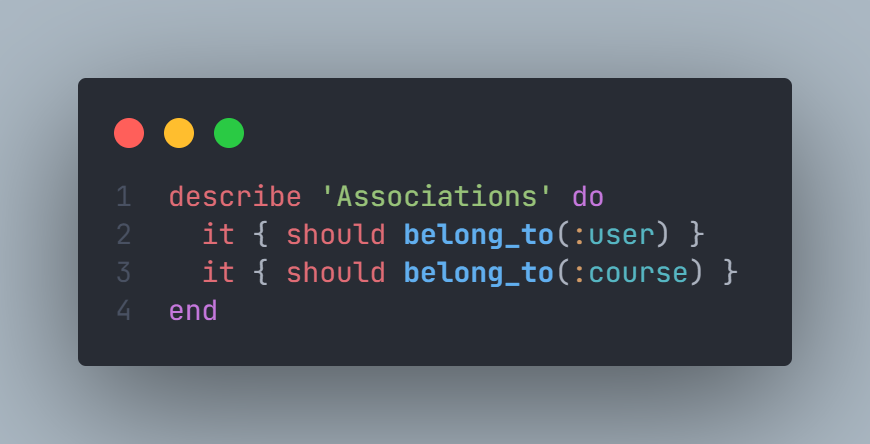
\includegraphics[width=140mm,scale=1]{figures/implementation_and_testing/testing/AUT/enrollment/associations.png}}
        \caption{Enrollment Model - Association Unit Tests}
        \label{Enrollment Model - Association Unit Tests}
    \end{figure}

\vspace{0.25cm}
\noindent\textbf{\textit{\underline{One-to-one relationships:}}} The belong\_to test confirms that an instance of the Enrollment model can be associated with one instance of another model. In our test suite, it { should belong\_to(:user) } and it { should belong\_to(:course) } ascertain that an Enrollment instance can be linked with a particular User and Course.

    \begin{figure}[H]
        \centerline{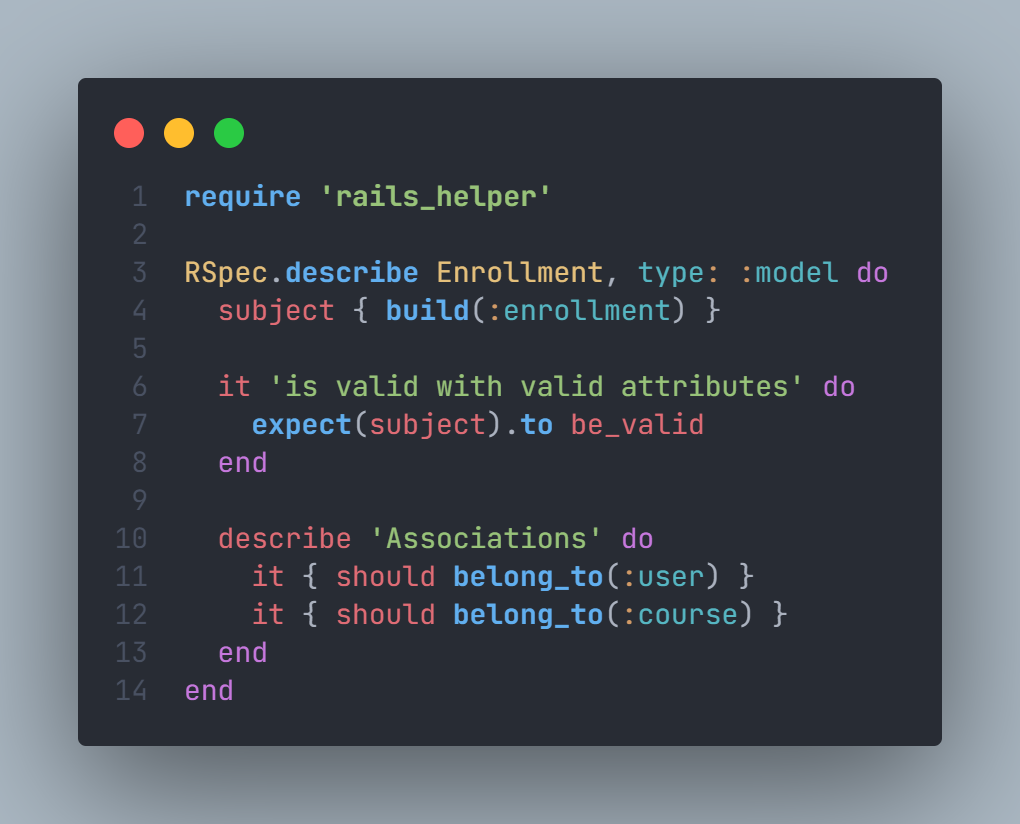
\includegraphics[width=140mm,scale=1]{figures/implementation_and_testing/testing/AUT/enrollment/all.png}}
        \caption{Enrollment Model Unit Tests}
        \label{Enrollment Model Unit Tests}
    \end{figure}


%%%%%%%%%%%%%%%%%%%%%%%%%%%%%%%%%%%%%%%%%%%%%%%%%%%%%%%%%%%%%%%%%
%%%%%%%%%%%%%%%%%%%%%%%%%%%%%%%%%%%%%%%%%%%%%%%%%%%%%%%%%%%%%%%%%


\newendline \textbf{\textit{Course Model}}\newendline
The unit tests that have been completed for the Course model are as follows.

\vspace{0.25cm}
\newendline
\textbf{Attribute Validations}

    \begin{figure}[H]
        \centerline{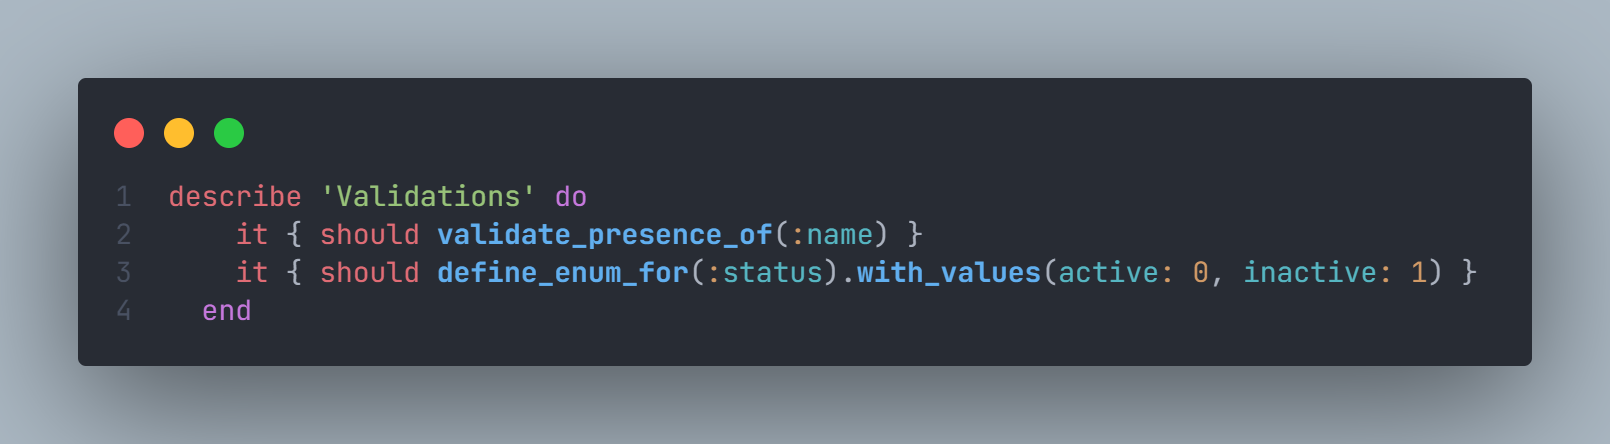
\includegraphics[width=140mm,scale=1]{figures/implementation_and_testing/testing/AUT/course/validations.png}}
        \caption{Course Model - Validation Unit Tests}
        \label{Course Model - Validation Unit Tests}
    \end{figure}

\vspace{-0.25cm}
\noindent\textbf{\textit{\underline{Presence validation:}}} The validate\_presence\_of test ensures that certain attributes are not empty. For example, validate\_presence\_of(:name) ensures that a Course instance cannot be saved without a name attribute.

\vspace{0.25cm}
\noindent\textbf{\textit{\underline{Enumeration validation:}}} The define\_enum\_for test validates enumerations, ensuring that a specific attribute maps certain names to integer values in the database. For example, define\_enum\_for(:status).with\_values(active: 0, inactive: 1) validates that the status attribute maps 'active' to 0 and 'inactive' to 1.

\vspace{0.25cm}
\newendline
\textbf{Model Associations}

    \begin{figure}[H]
        \centerline{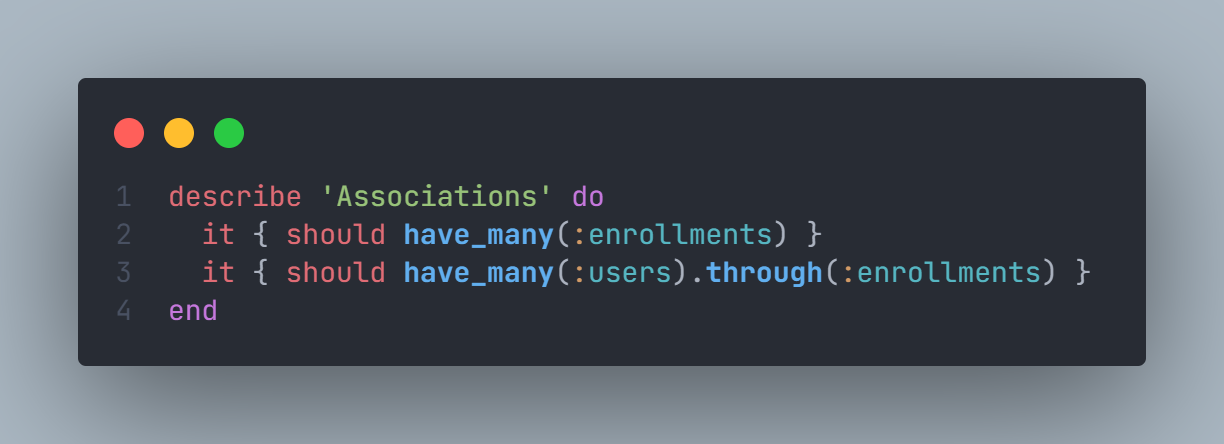
\includegraphics[width=140mm,scale=1]{figures/implementation_and_testing/testing/AUT/course/associations.png}}
        \caption{Course Model - Association Unit Tests}
        \label{Course Model - Association Unit Tests}
    \end{figure}

\vspace{0.25cm}
\noindent\textbf{\textit{\underline{One-to-many relationships:}}} The have\_many test verifies that an instance of the Course model can be associated with multiple instances of another model. In our suite, it { should have\_many(:enrollments) } confirms that a Course can have multiple Enrollments.

\vspace{0.25cm}
\noindent\textbf{\textit{\underline{Many-to-many relationships:}}} The have\_many...through test validates relationships where a Course instance can be associated with many instances of another model through a third model. In our test suite, it { should have\_many(:users).through(:enroll- ments) } asserts that a Course can be associated with many Users through Enrollments.


    \begin{figure}[H]
        \centerline{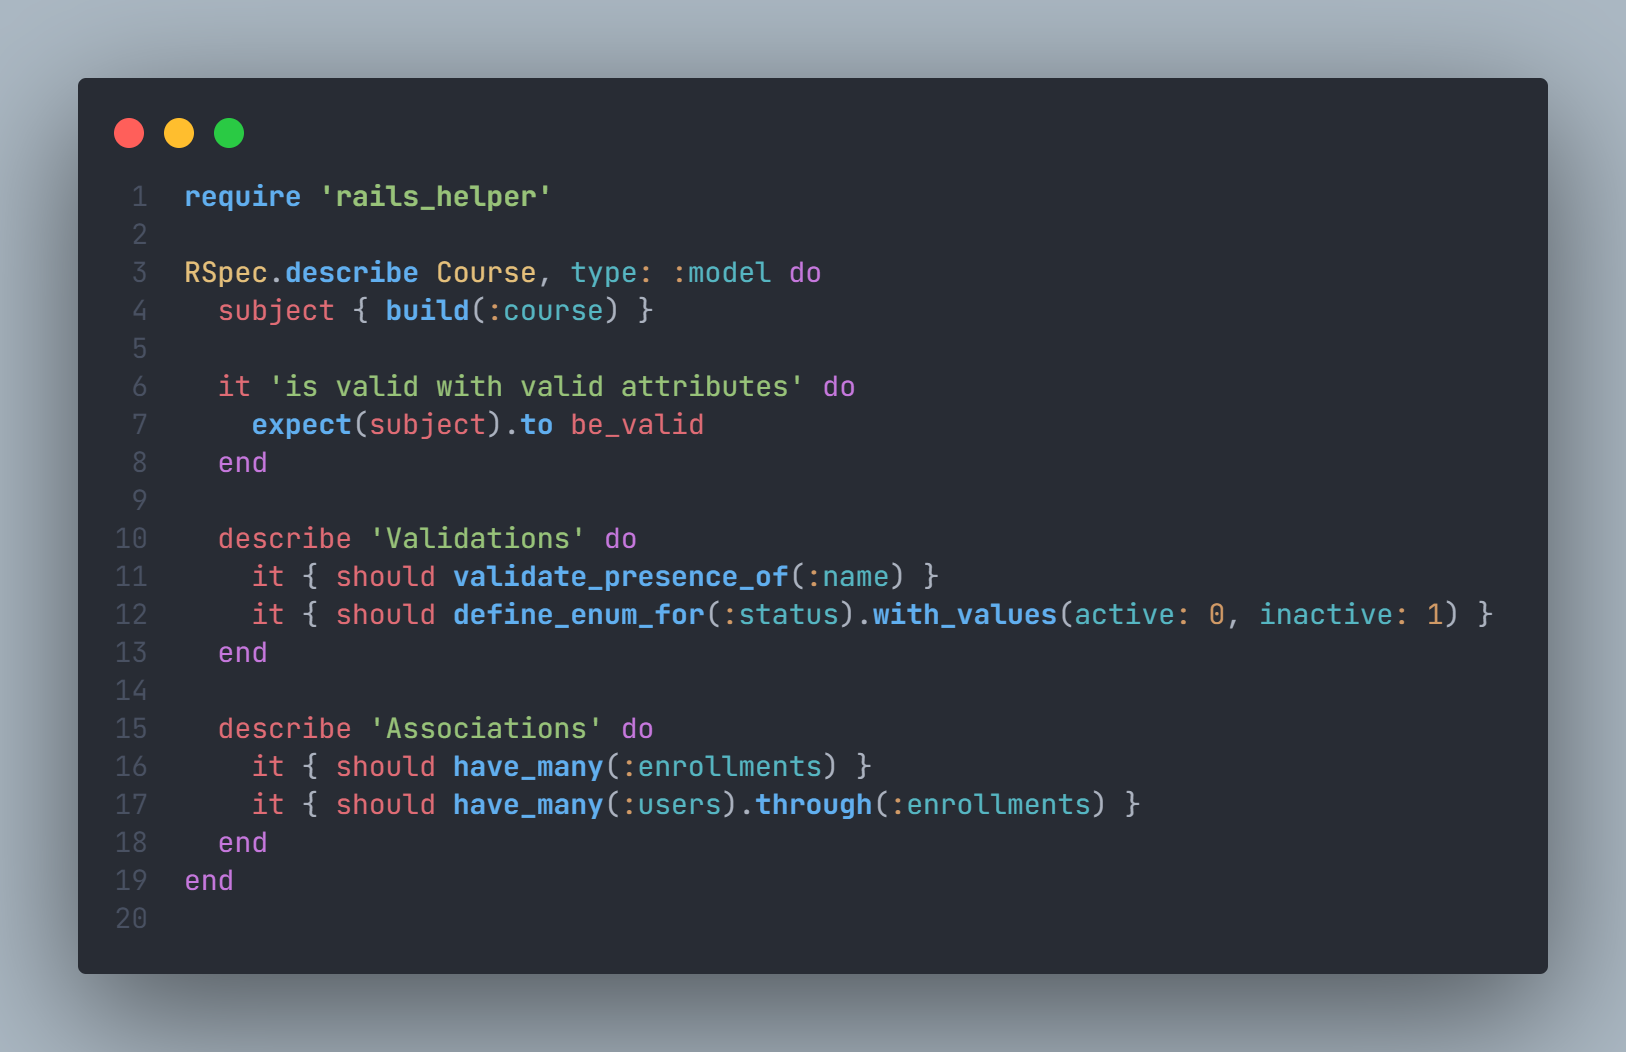
\includegraphics[width=140mm,scale=1]{figures/implementation_and_testing/testing/AUT/course/all.png}}
        \caption{Course Model Unit Tests}
        \label{Course Model Unit Tests}
    \end{figure}



%%%%%%%%%%%%%%%%%%%%%%%%%%%%%%%%%%%%%%%%%%%%%%%%%%%%%%%%%%%%%%%%%
%%%%%%%%%%%%%%%%%%%%%%%%%%%%%%%%%%%%%%%%%%%%%%%%%%%%%%%%%%%%%%%%%



\newendline \textbf{\textit{Attendance Model}}\newendline
The unit tests that have been completed for the Attendance model are as follows.

\vspace{0.25cm}
\newendline
\textbf{Attribute Validations}

    \begin{figure}[H]
        \centerline{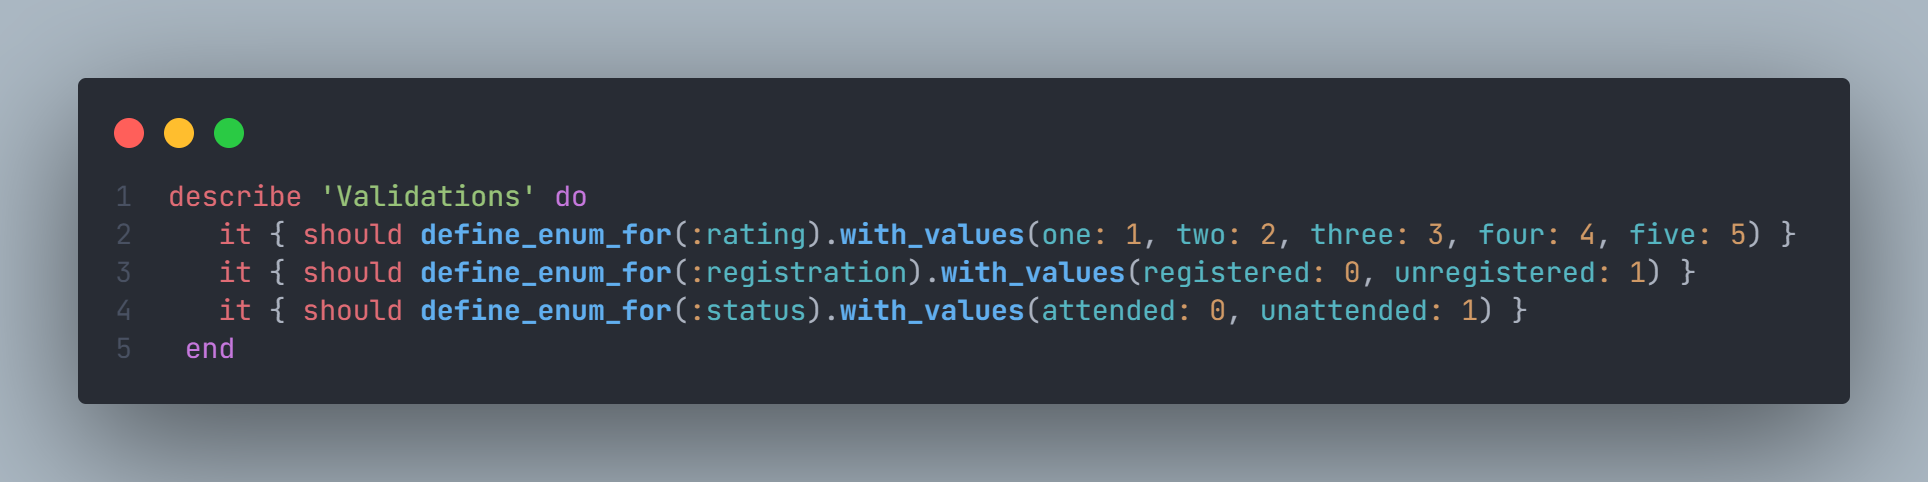
\includegraphics[width=140mm,scale=1]{figures/implementation_and_testing/testing/AUT/attendance/validations.png}}
        \caption{Attendance Model - Validation Unit Tests}
        \label{Attendance Model - Validation Unit Tests}
    \end{figure}

\vspace{0.25cm}
\noindent\textbf{\textit{\underline{Enumeration validation:}}} This model utilizes define\_enum\_for to validate three enumerations. The first test, define\_enum\_for(:rating).with\_values(one: 1, two: 2, three: 3, four: 4, five: 5), ensures that the rating attribute maps the numbers from one to five correctly. The second test, define\_enum\_for(:registration).with\_values(registered: 0, unregistered: 1), verifies that the registration attribute maps 'registered' to 0 and 'unregistered' to 1. The last test, define\_enum\_for(:status).with\_values(attended: 0, unattended: 1), confirms that the status attribute maps 'attended' to 0 and 'unattended' to 1.

\vspace{0.25cm}
\newendline
\textbf{Model Associations}

    \begin{figure}[H]
        \centerline{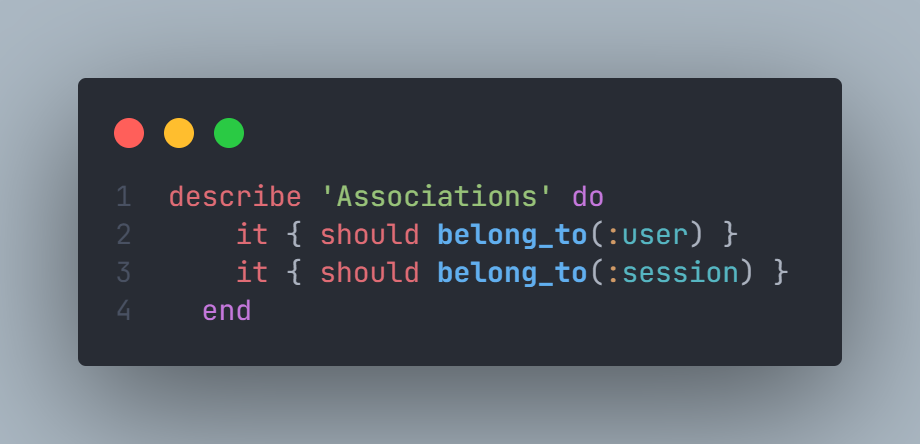
\includegraphics[width=140mm,scale=1]{figures/implementation_and_testing/testing/AUT/attendance/associations.png}}
        \caption{Attendance Model - Association Unit Tests}
        \label{Attendance Model - Association Unit Tests}
    \end{figure}

\vspace{0.25cm}
\noindent\textbf{\textit{\underline{One-to-one relationships:}}} This model has two belong\_to tests to confirm the association between the Attendance model and the User and Session models. The it { should belong\_to(:user) } and it { should belong\_to(:session) } tests ensure that each Attendance instance is associated with a single User and a single Session instance.


    \begin{figure}[H]
        \centerline{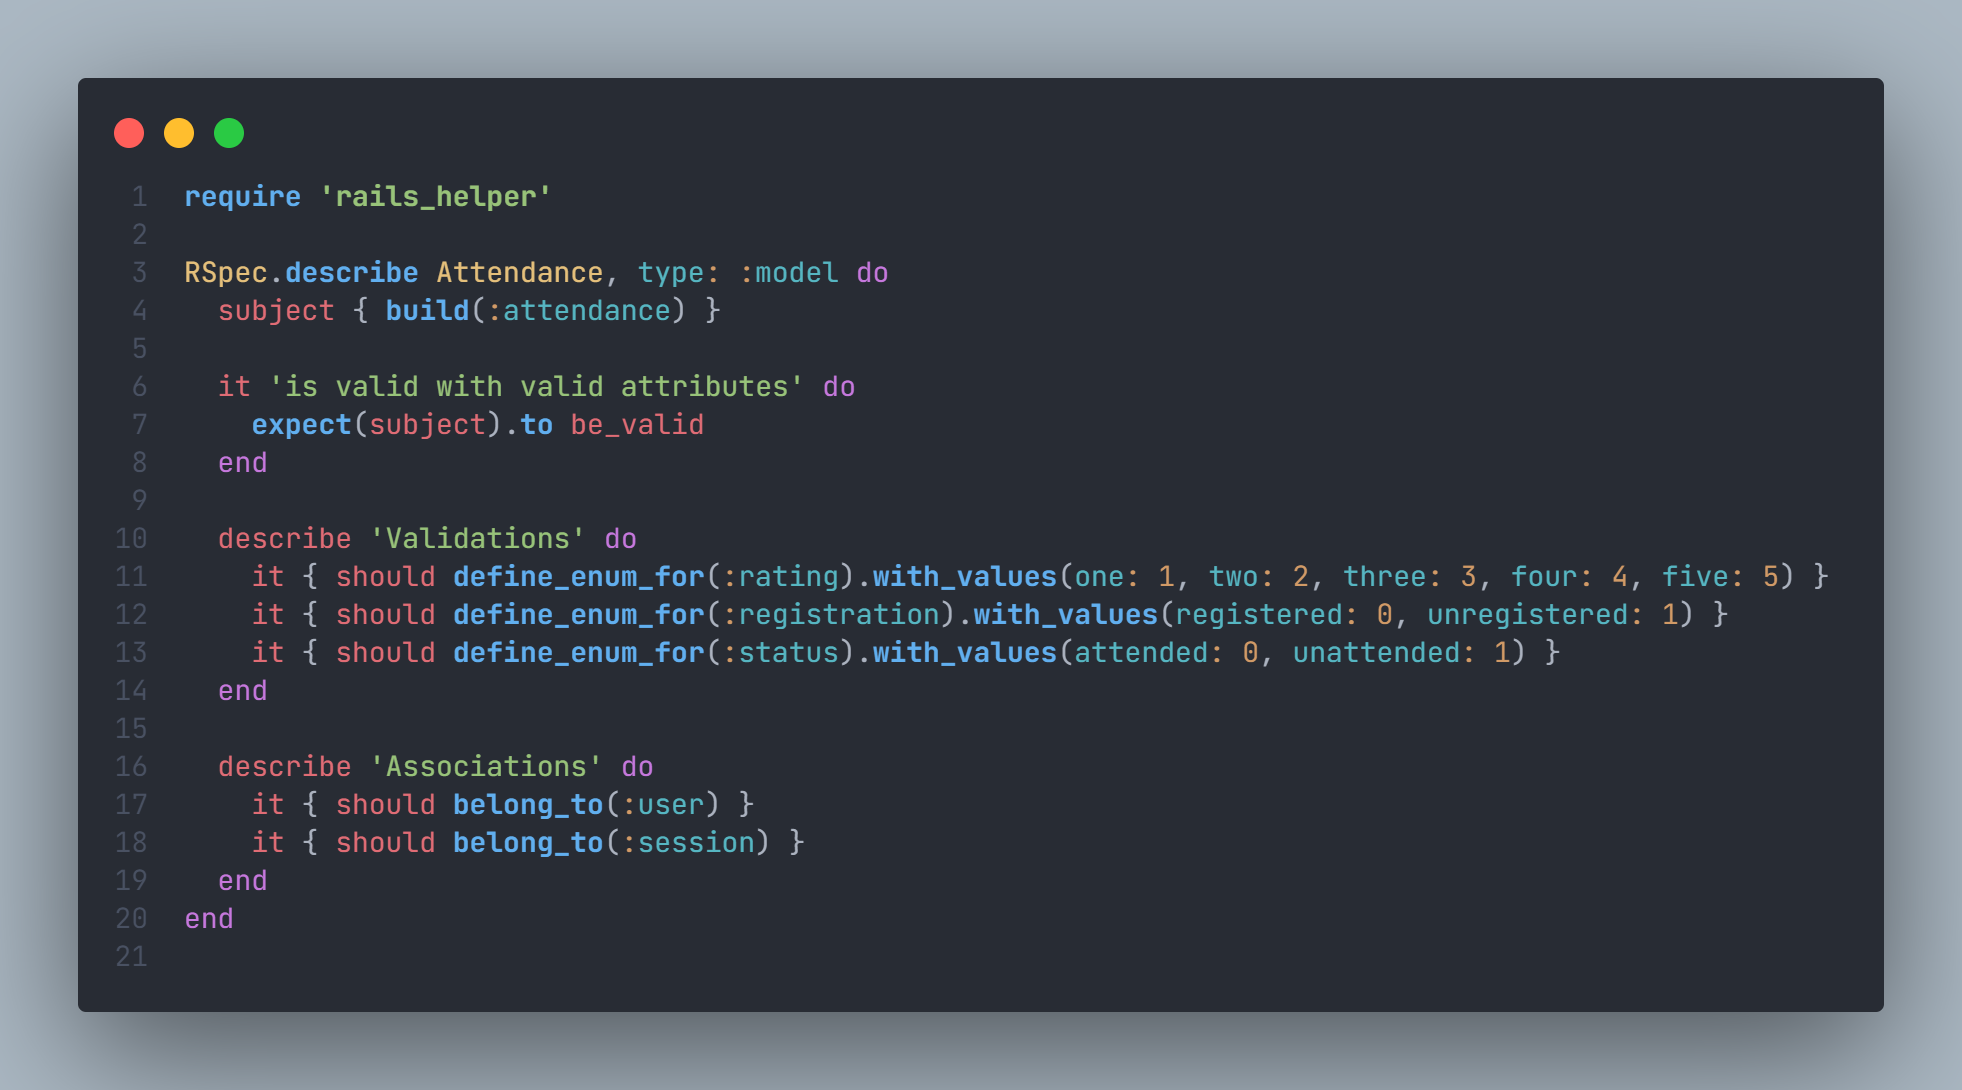
\includegraphics[width=140mm,scale=1]{figures/implementation_and_testing/testing/AUT/attendance/all.png}}
        \caption{Attendance Model Unit Tests}
        \label{Attendance Model Unit Tests}
    \end{figure}

%%%%%%%%%%%%%%%%%%%%%%%%%%%%%%%%%%%%%%%%%%%%%%%%%%%%%%%%%%%%%%%%%
%%%%%%%%%%%%%%%%%%%%%%%%%%%%%%%%%%%%%%%%%%%%%%%%%%%%%%%%%%%%%%%%%


\newendline \textbf{\textit{Answer Model}}\newendline
The unit tests that have been completed for the Answer model are as follows.

\vspace{0.25cm}
\newendline
\textbf{Attribute Validations}


    \begin{figure}[H]
        \centerline{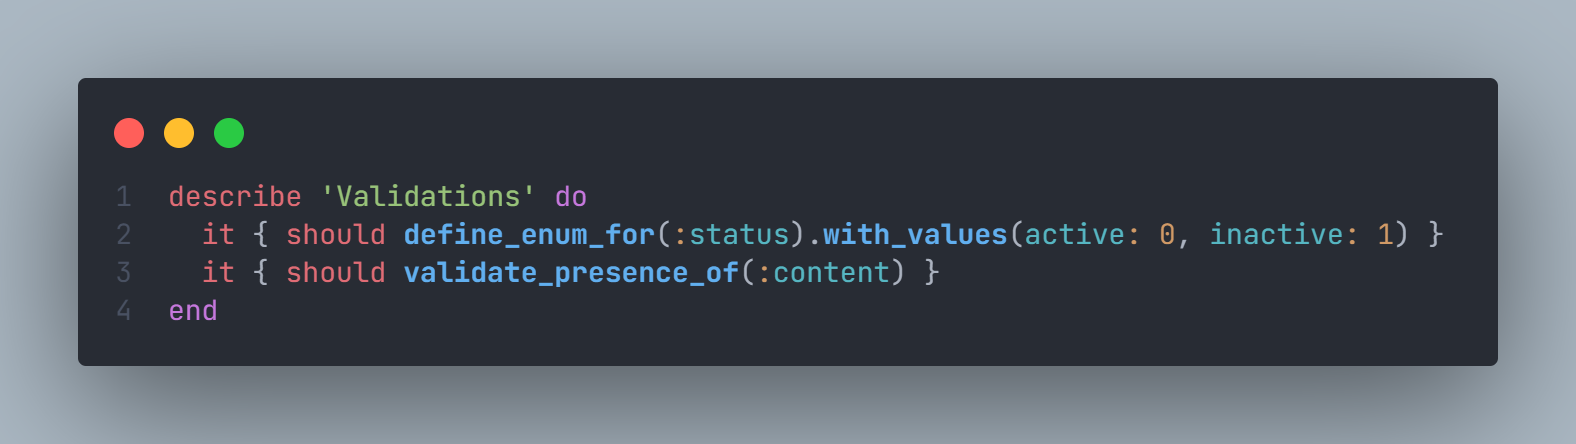
\includegraphics[width=140mm,scale=1]{figures/implementation_and_testing/testing/AUT/answer/validations.png}}
        \caption{Answer Model - Validation Unit Tests}
        \label{Answer Model - Validation Unit Tests}
    \end{figure}

\vspace{0.25cm}
\noindent\textbf{\textit{\underline{Presence validation:}}} The presence validation test validate\_presence\_of(:content) ensures that an Answer instance cannot be saved without the content attribute. This is crucial as each answer must have content to provide meaningful feedback.

\vspace{0.25cm}
\noindent\textbf{\textit{\underline{Enumeration validation:}}} This model uses define\_enum\_for to validate the status enumeration. The test define\_enum\_for(:status).with\_values(active: 0, inactive: 1) confirms that the status attribute accurately maps the terms 'active' and 'inactive' to 0 and 1 respectively.

\vspace{0.25cm}
\newendline
\textbf{Model Associations}

    \begin{figure}[H]
        \centerline{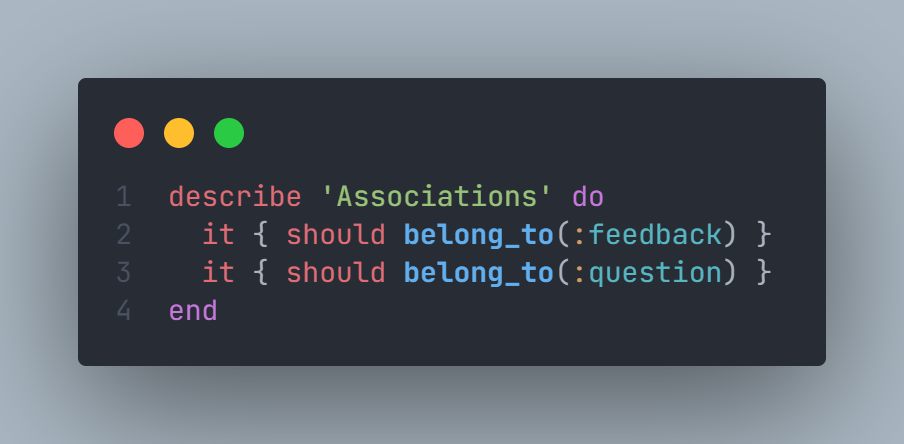
\includegraphics[width=140mm,scale=1]{figures/implementation_and_testing/testing/AUT/answer/associations.png}}
        \caption{Answer Model - Association Unit Tests}
        \label{Answer Model - Association Unit Tests}
    \end{figure}

\vspace{0.25cm}
\noindent\textbf{\textit{\underline{One-to-one relationships:}}} The Answer model has two belong\_to tests that confirm its associations with the Feedback and Question models. The it { should belong\_to(:feedback) } test ensures that each Answer instance is associated with a single Feedback instance, while the it { should belong\_to(:question) } test verifies that each Answer is associated with a single Question instance.

    \begin{figure}[H]
        \centerline{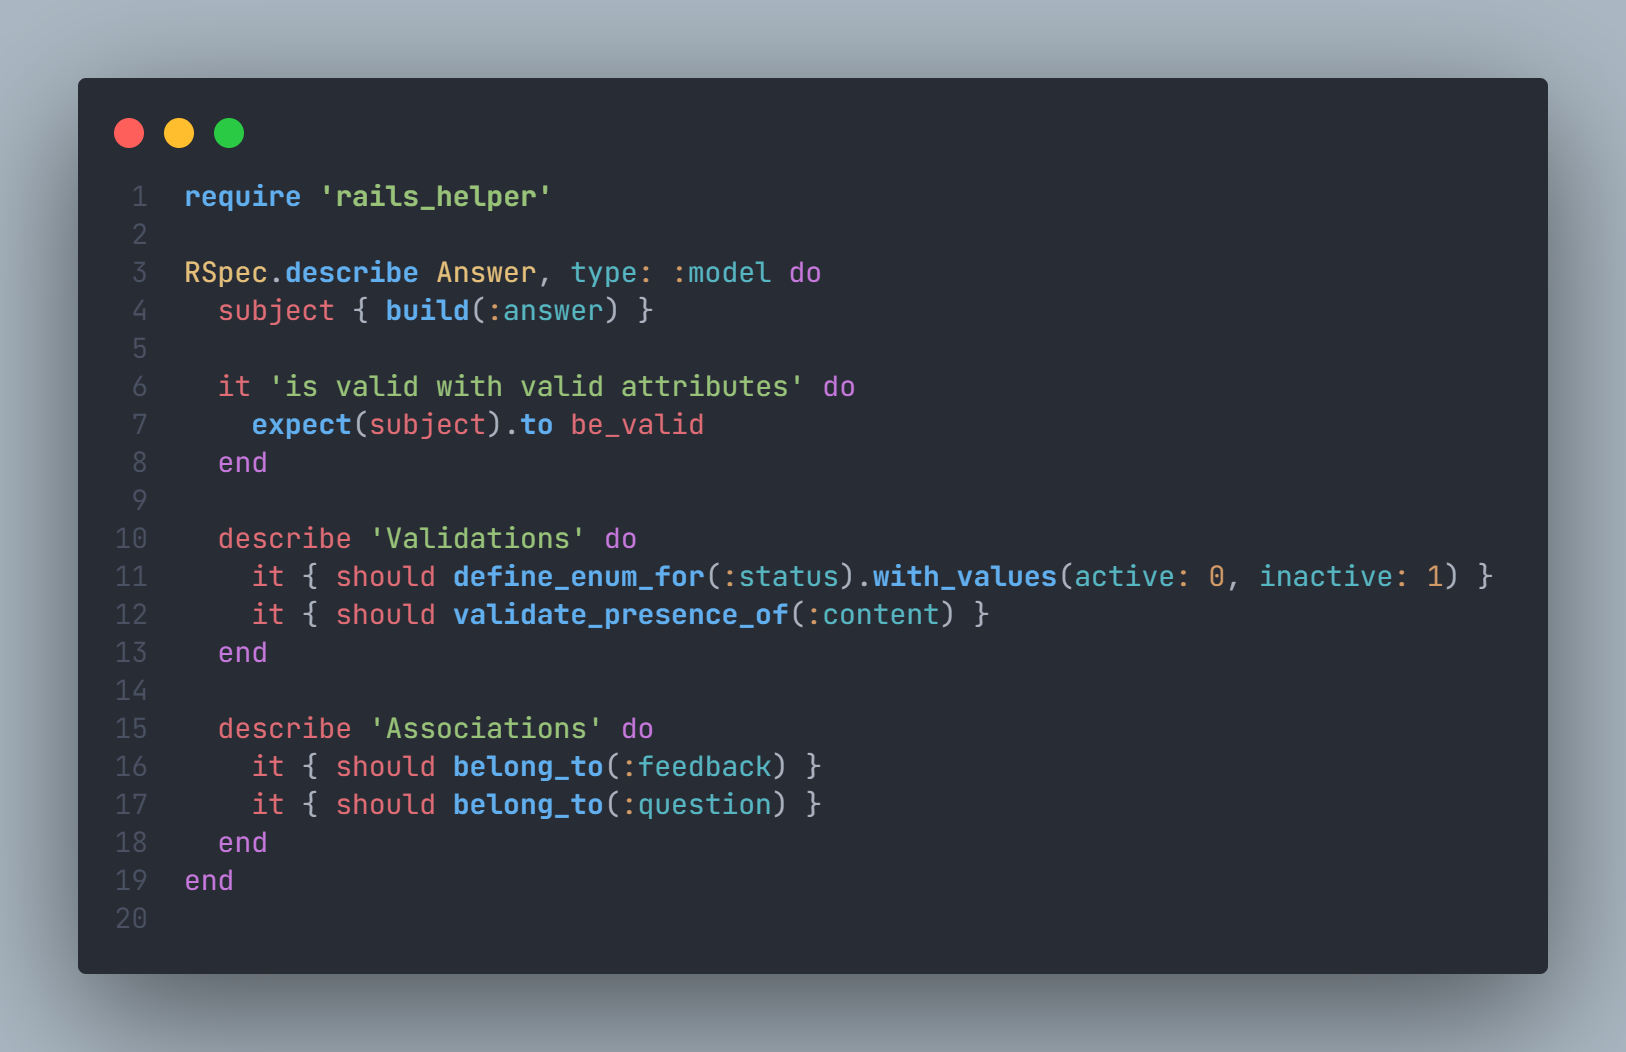
\includegraphics[width=140mm,scale=1]{figures/implementation_and_testing/testing/AUT/answer/all.png}}
        \caption{Answer Model Unit Tests}
        \label{Answer Model Unit Tests}
    \end{figure}

%%%%%%%%%%%%%%%%%%%%%%%%%%%%%%%%%%%%%%%%%%%%%%%%%%%%%%%%%%%%%%%%%
%%%%%%%%%%%%%%%%%%%%%%%%%%%%%%%%%%%%%%%%%%%%%%%%%%%%%%%%%%%%%%%%%


\newendline \textbf{\textit{Summary}}\newendline
Unit tests ensure that specific parts of the STDC application work as intended, which improves the application's overall reliability and stability. They assisted in the prevention of errors, the acceleration of development, and the preservation of application's quality.

\end{justify}
\clearpage


%%%%%%%%%%%%%%%%%%%%%%%%%%%%%%%%%%%%%%%%%%%%%%%%%%%%%%%%%%%%%%%%%
%%%%%%%%%%%%%%%%%%%%%%%%%%%%%%%%%%%%%%%%%%%%%%%%%%%%%%%%%%%%%%%%%
%%%%%%%%%%%%%%%%%%%%%%%%%%%%%%%%%%%%%%%%%%%%%%%%%%%%%%%%%%%%%%%%%
%%%%%%%%%%%%%%%%%%%%%%%%%%%%%%%%%%%%%%%%%%%%%%%%%%%%%%%%%%%%%%%%%

\vspace{0.25cm}
\subsection{Integration Testing}
\begin{justify}
Integration testing is a crucial aspect of testing of the Student Talent Development Center (STDC), offering a mechanism to combine individual units of the STDC application and tests them as a group. It is particularly valuable for catching issues that may have been missed during unit testing, and ensures that the various parts of the STDC application interact correctly. Since STDC's backend uses the Ruby on Rails framework, these components are represented by the controllers. Here, we will explore the integration testing strategies applied to one of the key controllers (Course). The testing is facilitated by the RSpec testing framework, enhanced by the RSwag gem, which aids in creating clean, readable, and effective test cases as well as swagger documentations based on the integration test cases.

\newendline Please note that only Course integration test has been highlighted below, however the rest of the integration tests can be found in the “stdc-api” repository that is available on github.

\vspace{0.25cm}
\newendline \textbf{\textit{Common Testing Aspects (Setups)}}\newendline
Below here are line that you might see being repeated in almost all the test cases, for now, the course integration test is taken as an example, however the rest should be the same.

\begin{figure}[H]
    \centerline{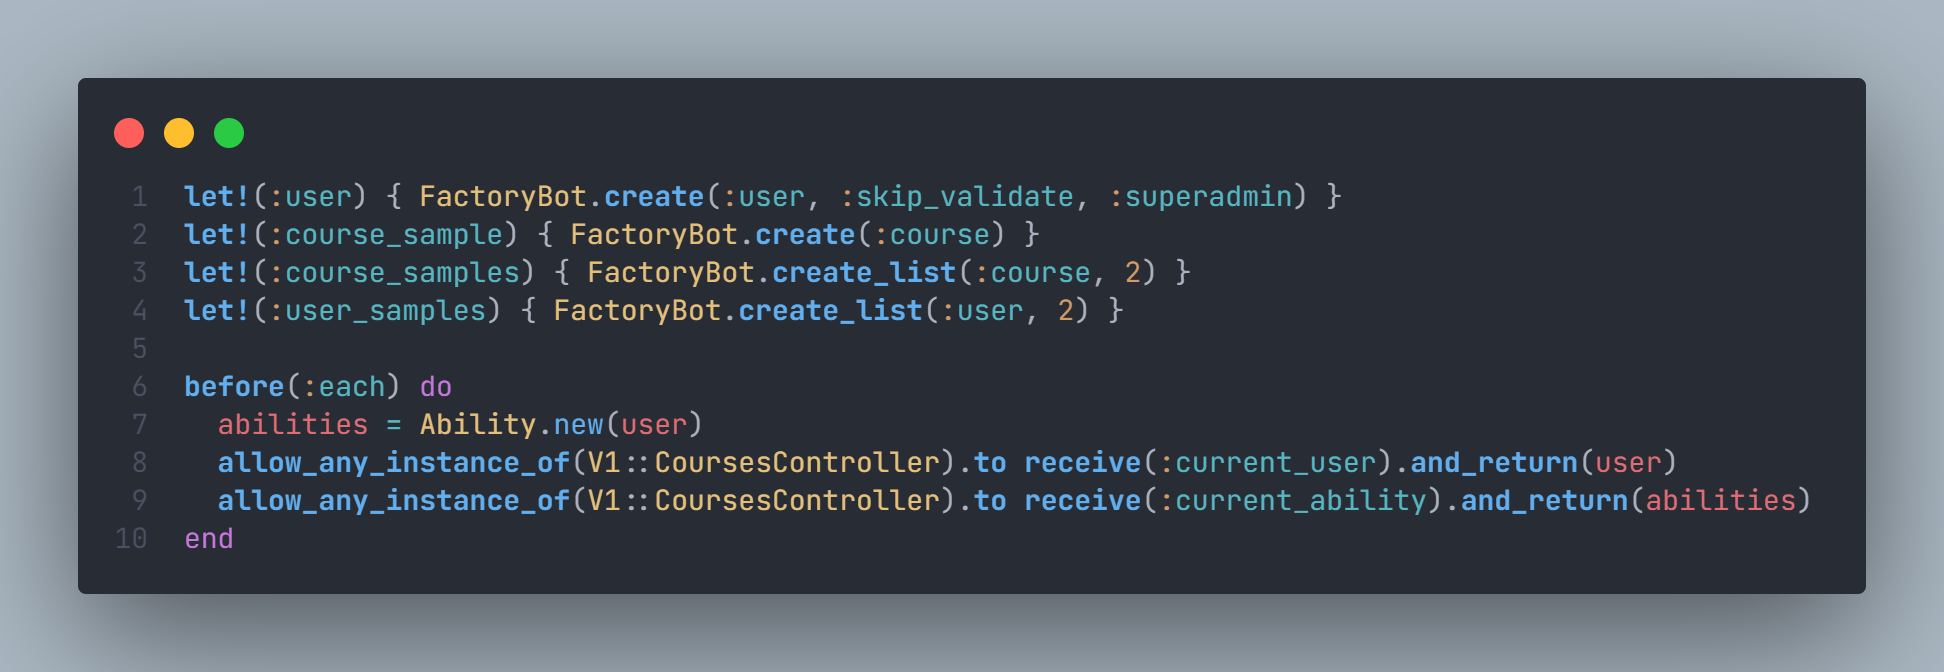
\includegraphics[width=150mm,scale=1]{figures/implementation_and_testing/testing/AIT/CommonAspects.png}}
    \caption{Automated Integration Testing - Setup}
    \label{Automated Integration Testing - Setup}
\end{figure}

\clearpage
\begin{enumerate}
    \item let!(:user) { FactoryBot.create(:user, :skip\_validate, :superadmin) }: This line is using FactoryBot, a testing utility, to create a user. The symbols :skip\_validate and :superadmin are traits defined in the FactoryBot configurations for user creation. This line creates a dummy user with the role of the superadmin to have access to everything. Additionally, validation for this user is skip on creation since the data used for creating the user are generated from Faker and do not reflect/represent real data.
    \vspace{0.25cm}

    \item let!(:course\_sample) { FactoryBot.create(:course) }: This line is creating a single Course instance using FactoryBot which is used later on for testing endpoints that return one single object, such as show, create, update, etc.
    \vspace{0.25cm}

    \item let!(:course\_samples) { FactoryBot.create\_list(:course, 2) }: This line is using FactoryBot to create a list of two Course instances which are used later on for testing endpoints that return more than one object (a collection of objects) such as index endpoint.
    \vspace{0.25cm}

    \item The before(:each) block is run before each test case (each it block). In this particular application, almost all before(:each) block is creating a new instance of Ability with the user created earlier and then stubbing (or mocking) some methods:
    \vspace{0.25cm}

    \item abilities = Ability.new(user): This line creates a new instance of Ability, a class to allow for user permissions and roles, using the previously created user with the help of the cancancan gem.
    \vspace{0.25cm}

    \item allow\_any\_instance\_of(V1::CoursesController).to receive(:current\_user).and - \_return(user): This line is stubbing the current\_user method on any instance of V1::CoursesController to return the user created earlier. This allows you to control the current user in the context of these tests, without having to go through the normal process of signing in or validation since this is a testing process.
    \vspace{0.25cm}
\clearpage
    \item allow\_any\_instance\_of(V1::CoursesController).to receive(:current\_ability).and- \_return(abilities): Similar to the previous line, this line is stubbing the current\_- ability method on any instance of V1::CoursesController to return the abilities object created earlier to grant the user permission.
\end{enumerate}

\vspace{0.25cm}
\newendline This setup ensures that each test runs in the context of a specific user (a superadmin, in this case) with a specific set of abilities, and with some specific course and user instances available. Please note that we only took Course as an example, other classes also have this setup for their integration tests.


\vspace{0.25cm}
\newendline \textbf{\textit{Course Model}}\newendline

\begin{figure}[H]
    \centerline{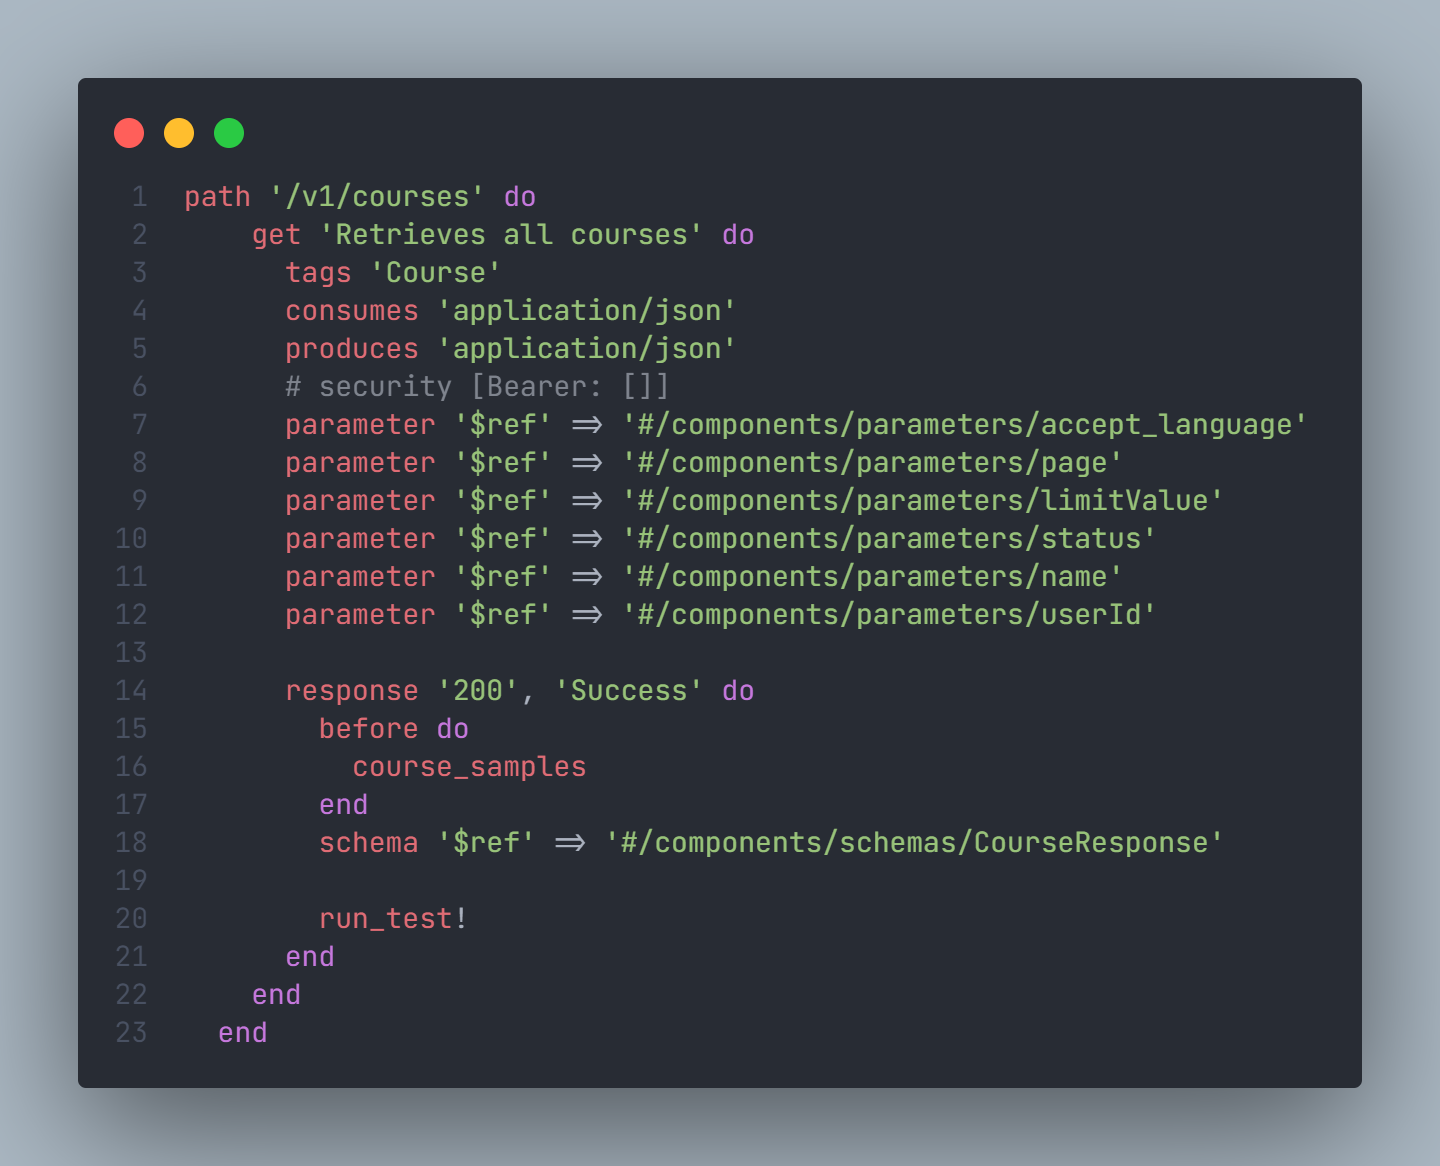
\includegraphics[width=150mm,scale=1]{figures/implementation_and_testing/testing/AIT/get_v1_courses.png}}
    \caption{Course Integration Testing - Get All Courses}
    \label{Course Integration Testing - Get All Courses}
\end{figure}

\noindent \textbf{GET /v1/courses:} This test case is checking if the application correctly retrieves all the courses. If the courses are successfully retrieved, a status of 200 and a JSON object containing all courses should be returned.

\begin{figure}[H]
    \centerline{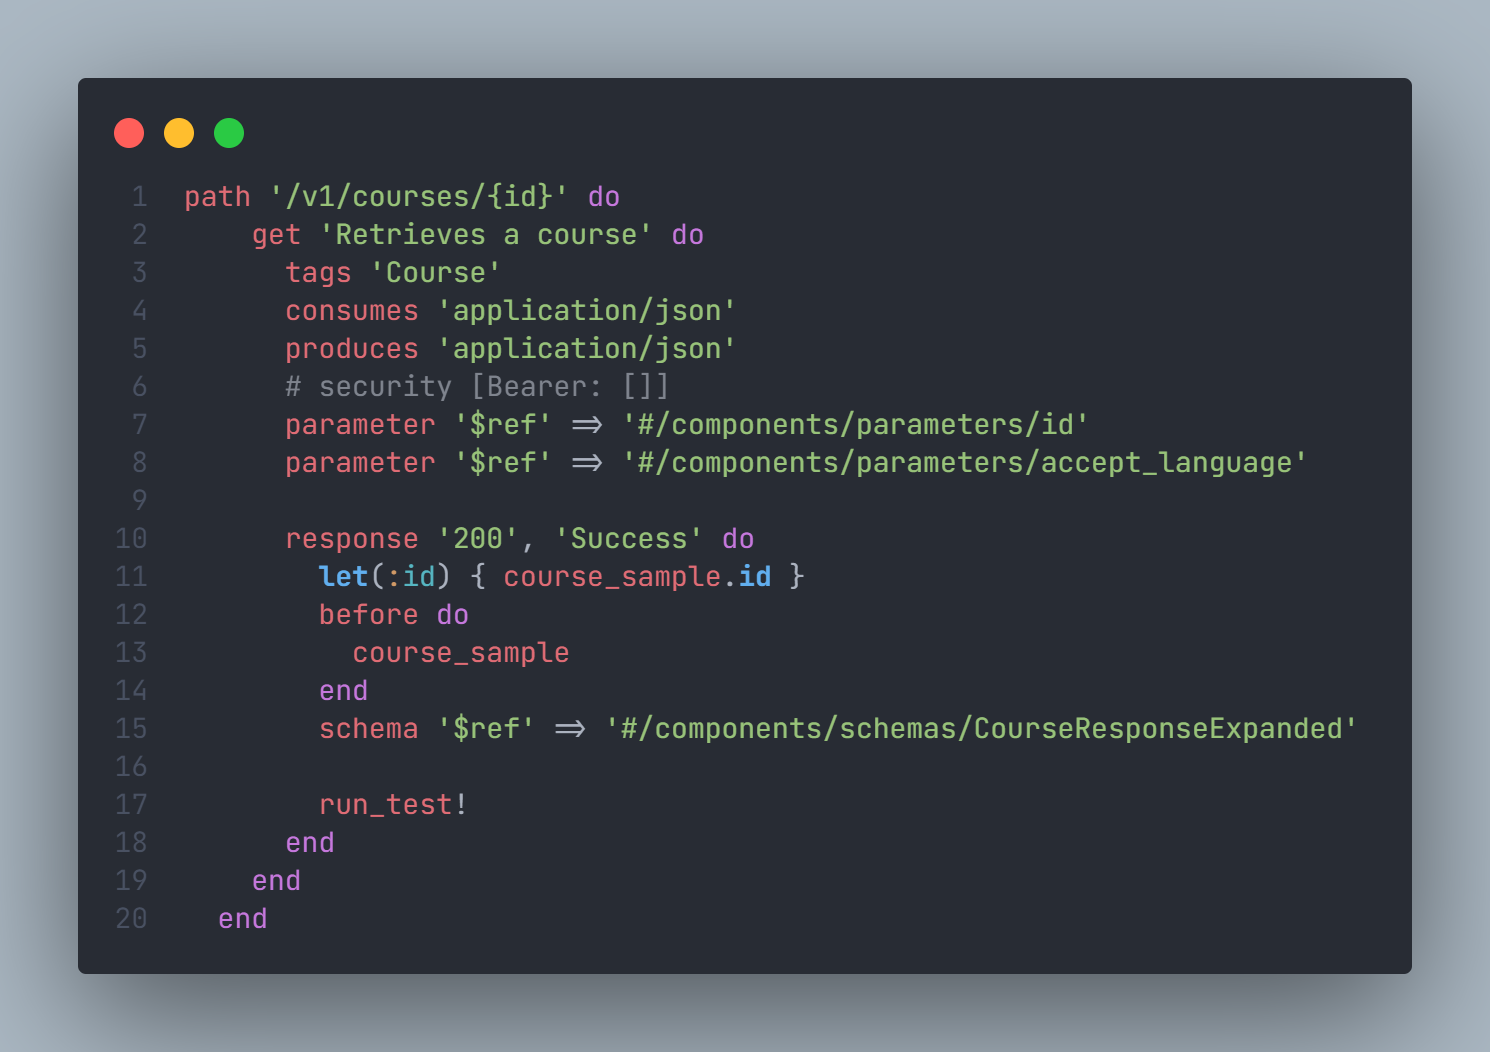
\includegraphics[width=150mm,scale=1]{figures/implementation_and_testing/testing/AIT/get_v1_course.png}}
    \caption{Course Integration Testing - Get Course By ID}
    \label{Course Integration Testing - Get Course By ID}
\end{figure}

\noindent \textbf{GET /v1/courses/{id}:} This test case verifies that a course can be retrieved individually using its id. If the specified course exists, it should return a 200 status and the JSON object of the course.

\begin{figure}[H]
    \centerline{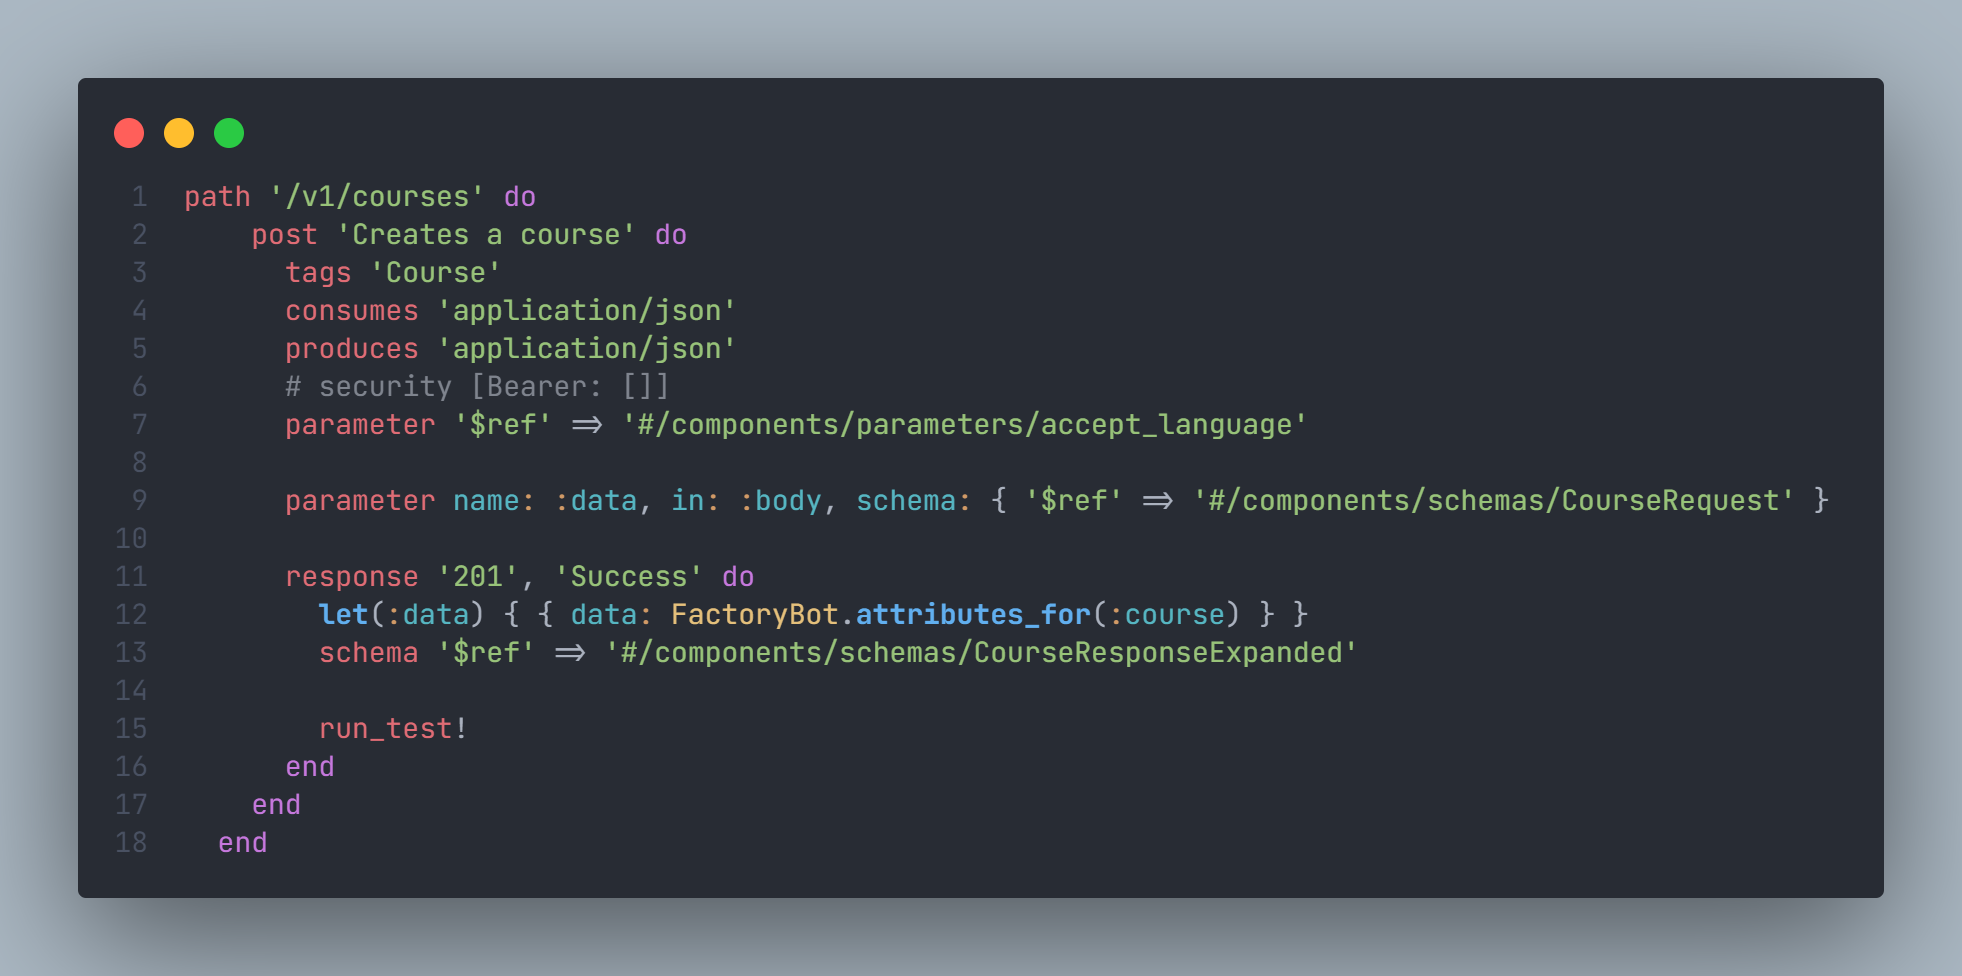
\includegraphics[width=150mm,scale=1]{figures/implementation_and_testing/testing/AIT/post_v1_courses.png}}
    \caption{Course Integration Testing - Create Courses}
    \label{Course Integration Testing - Create Courses}
\end{figure}

\noindent \textbf{POST /v1/courses:} This test case is checking if a course can be successfully created. The test data for the course is passed in the request body. If the course is created successfully, it should return a 201 status and the JSON object of the created course.

\begin{figure}[H]
    \centerline{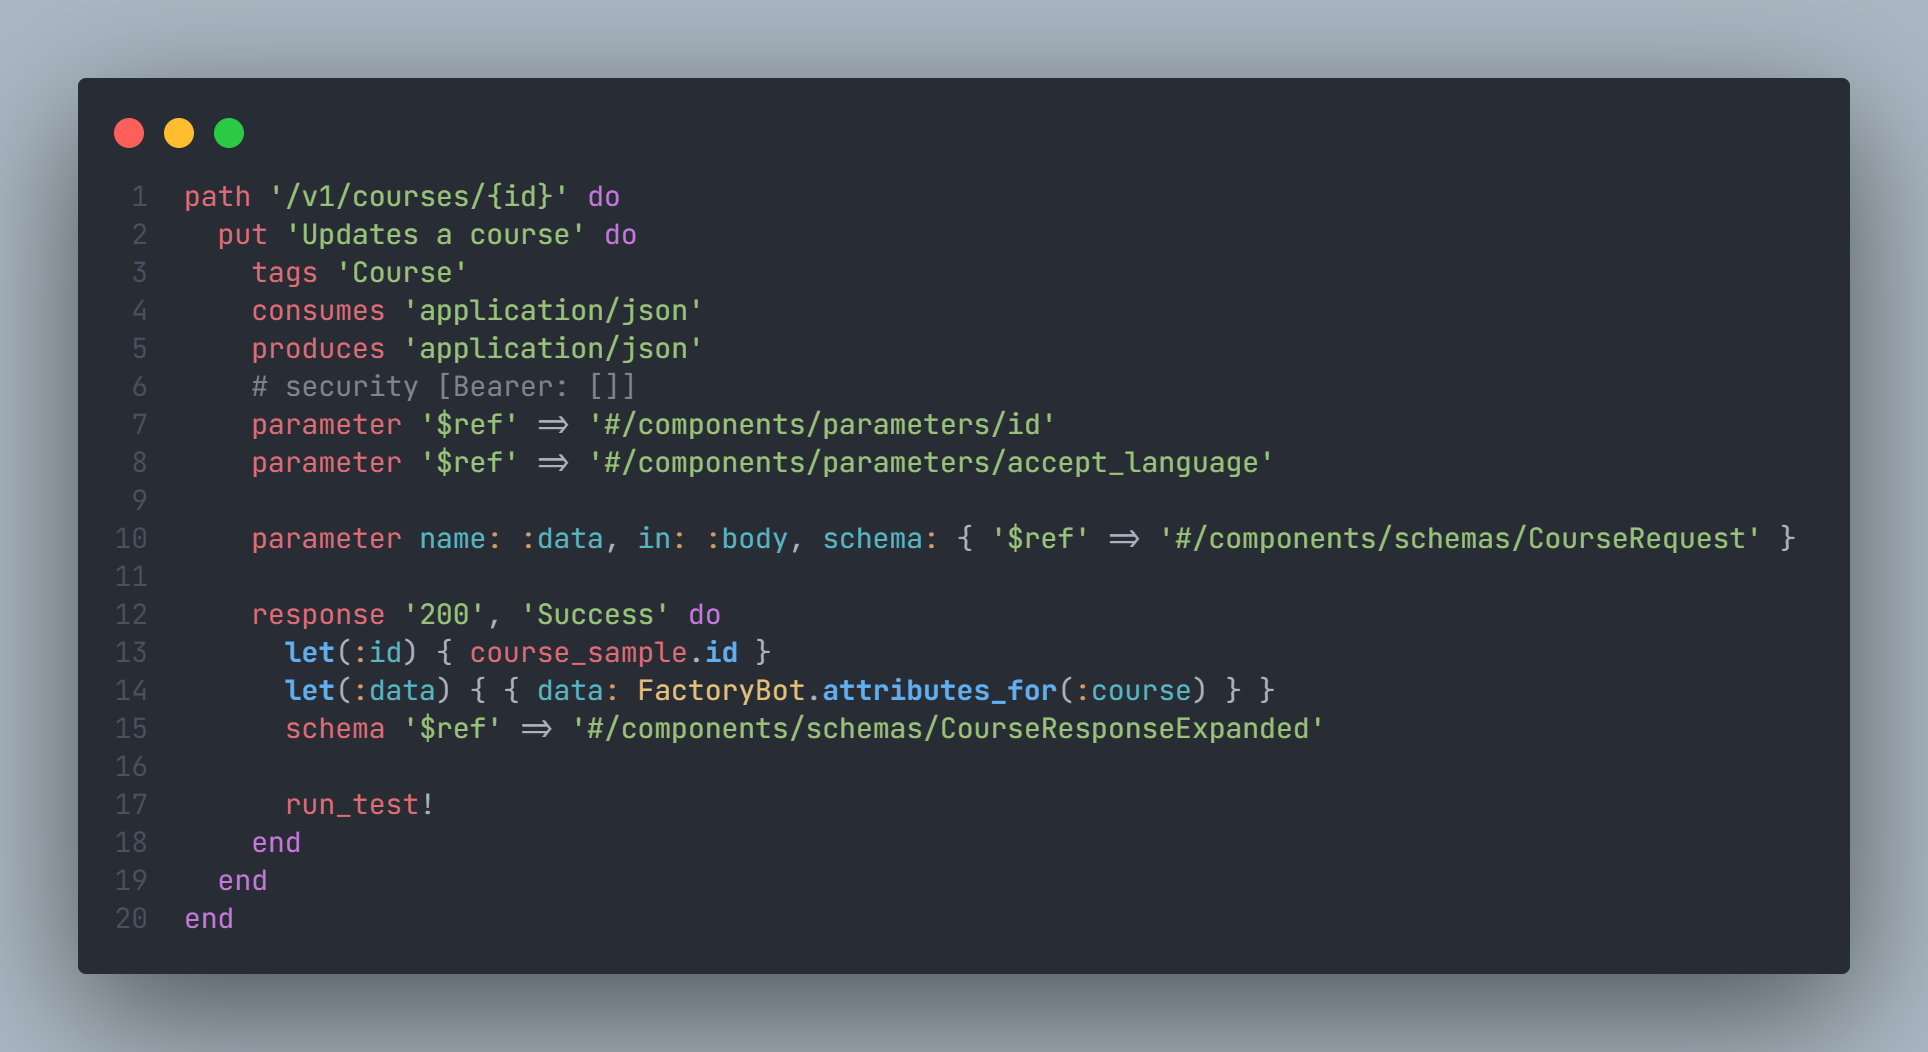
\includegraphics[width=150mm,scale=1]{figures/implementation_and_testing/testing/AIT/put_v1_course.png}}
    \caption{Course Integration Testing - Update Course}
    \label{Course Integration Testing - Update Course}
\end{figure}

\noindent \textbf{PUT /v1/courses/{id}:} This test case verifies that an existing course can be updated. The new data for the course is passed in the request body. If the course is updated successfully, it should return a 200 status and the JSON object of the updated course.

\begin{figure}[H]
    \centerline{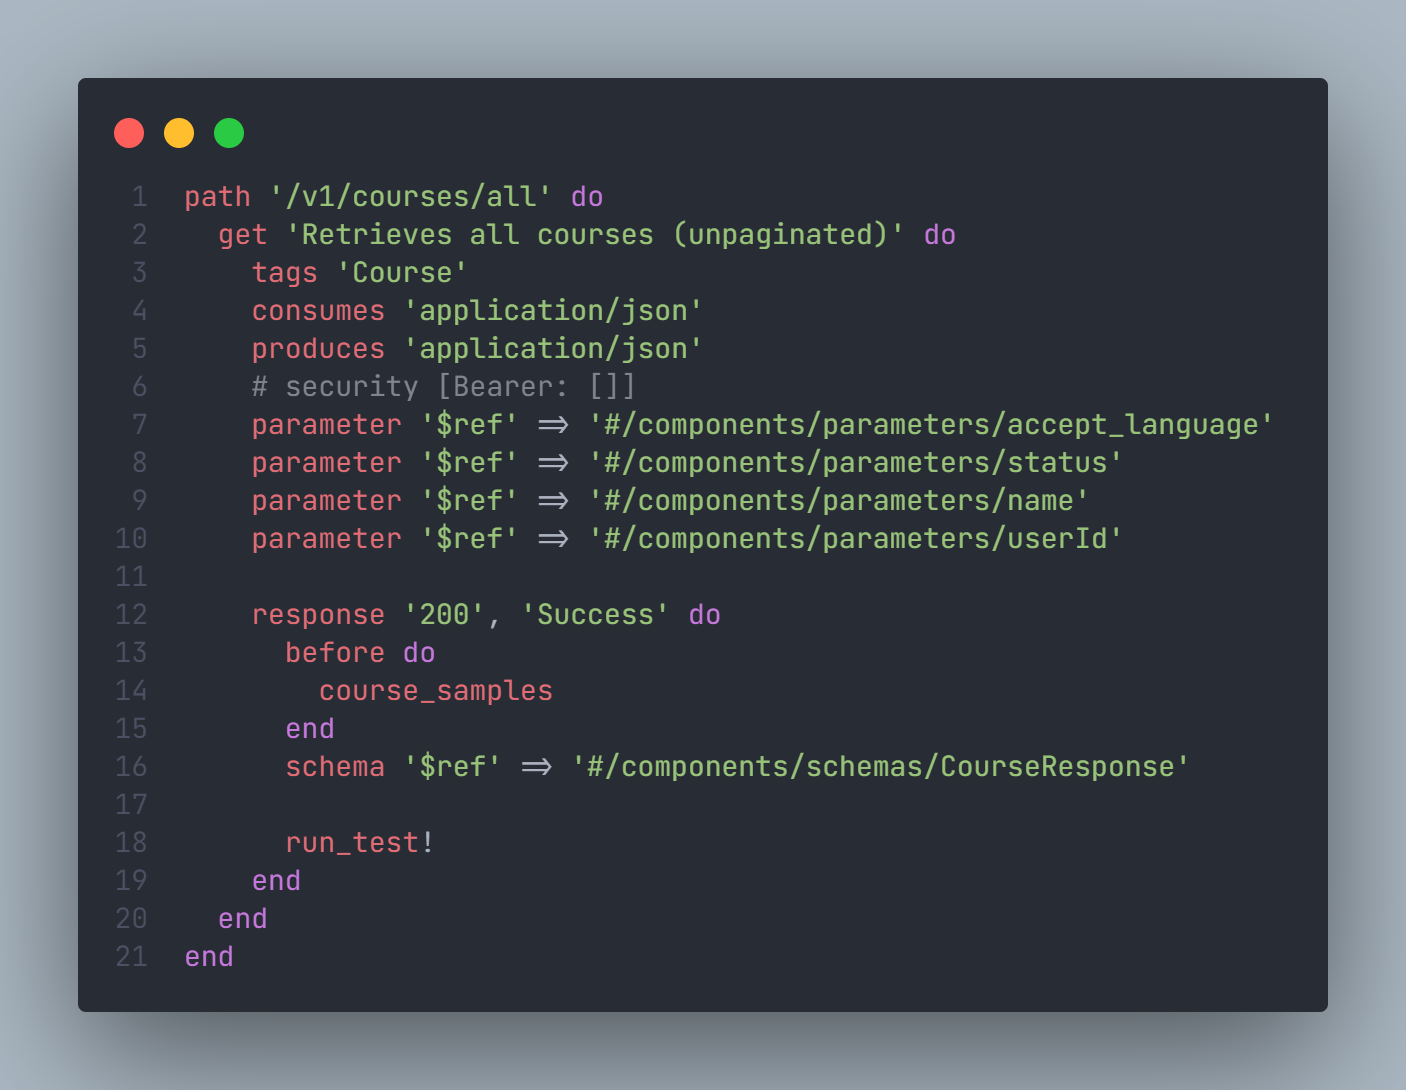
\includegraphics[width=150mm,scale=1]{figures/implementation_and_testing/testing/AIT/get_v1_all.png}}
    \caption{Course Integration Testing - Get All Courses With No Pagination}
    \label{Course Integration Testing - Get All Courses With No Pagination}
\end{figure}


\noindent \textbf{GET /v1/courses/all:} This test case is checking if all the courses can be retrieved without pagination. If the courses are successfully retrieved, a status of 200 and a JSON object containing all courses should be returned.

\begin{figure}[H]
    \centerline{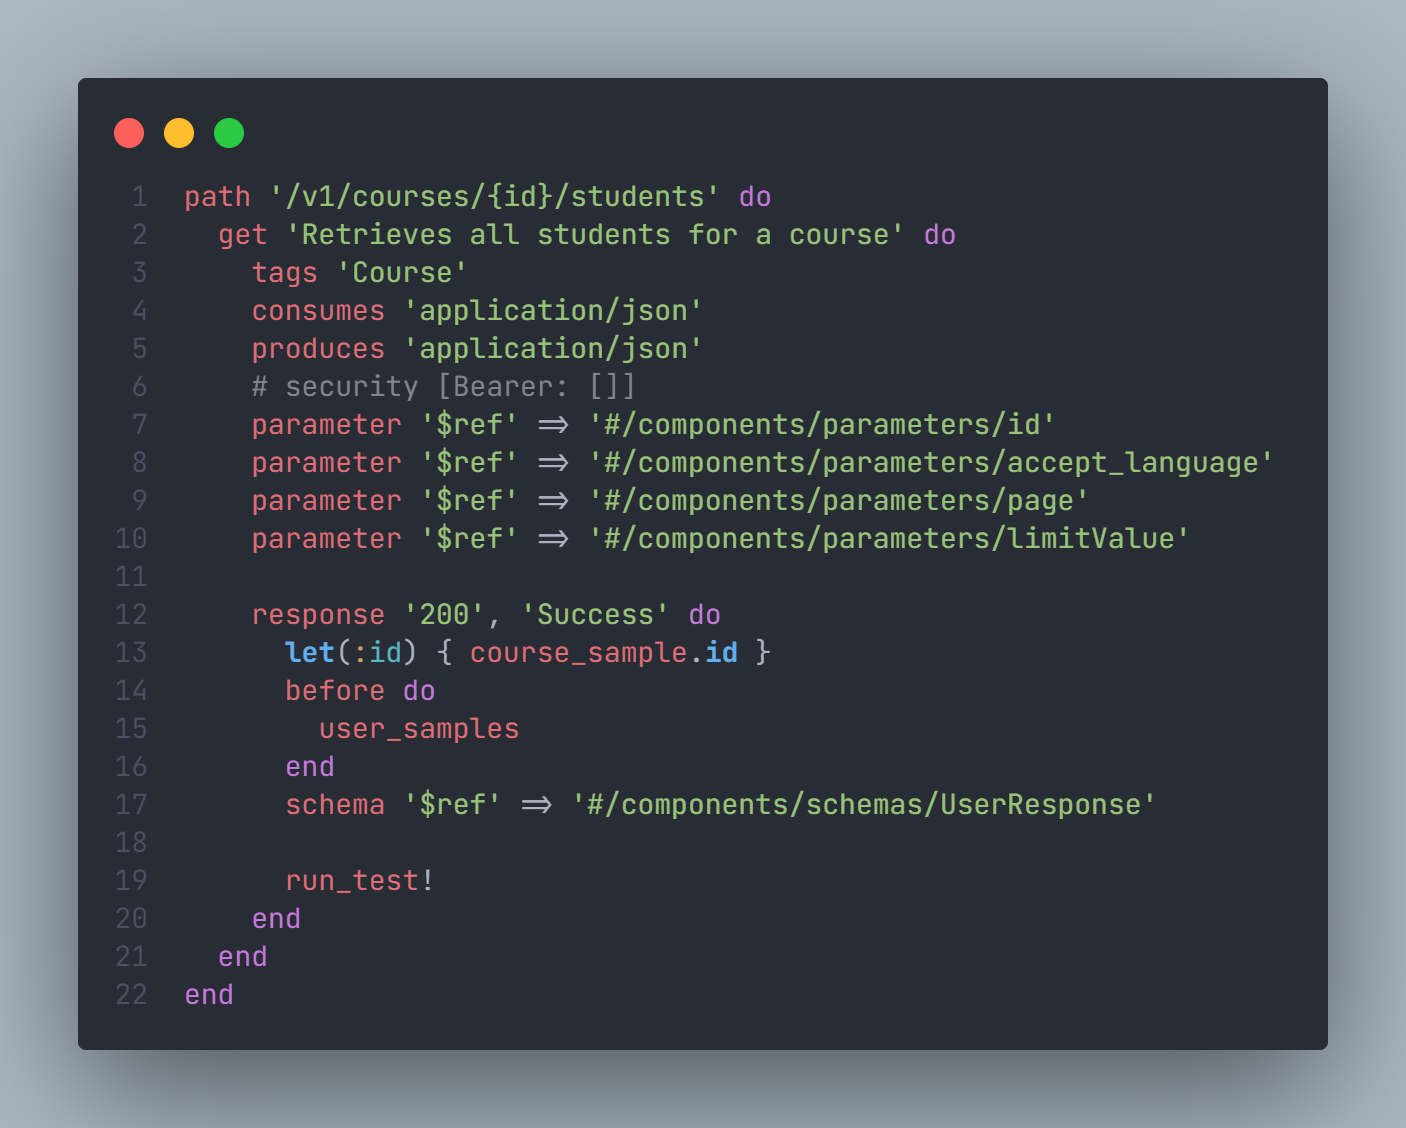
\includegraphics[width=150mm,scale=1]{figures/implementation_and_testing/testing/AIT/get_v1_students.png}}
    \caption{Course Integration Testing - Get All Students}
    \label{Course Integration Testing - Get All Students}
\end{figure}

\noindent \textbf{GET /v1/courses/{id}/students:} This test case is to verify that all students for a particular course can be retrieved. If the students are successfully retrieved, a 200 status and a JSON object containing all students in the course should be returned.

\begin{figure}[H]
    \centerline{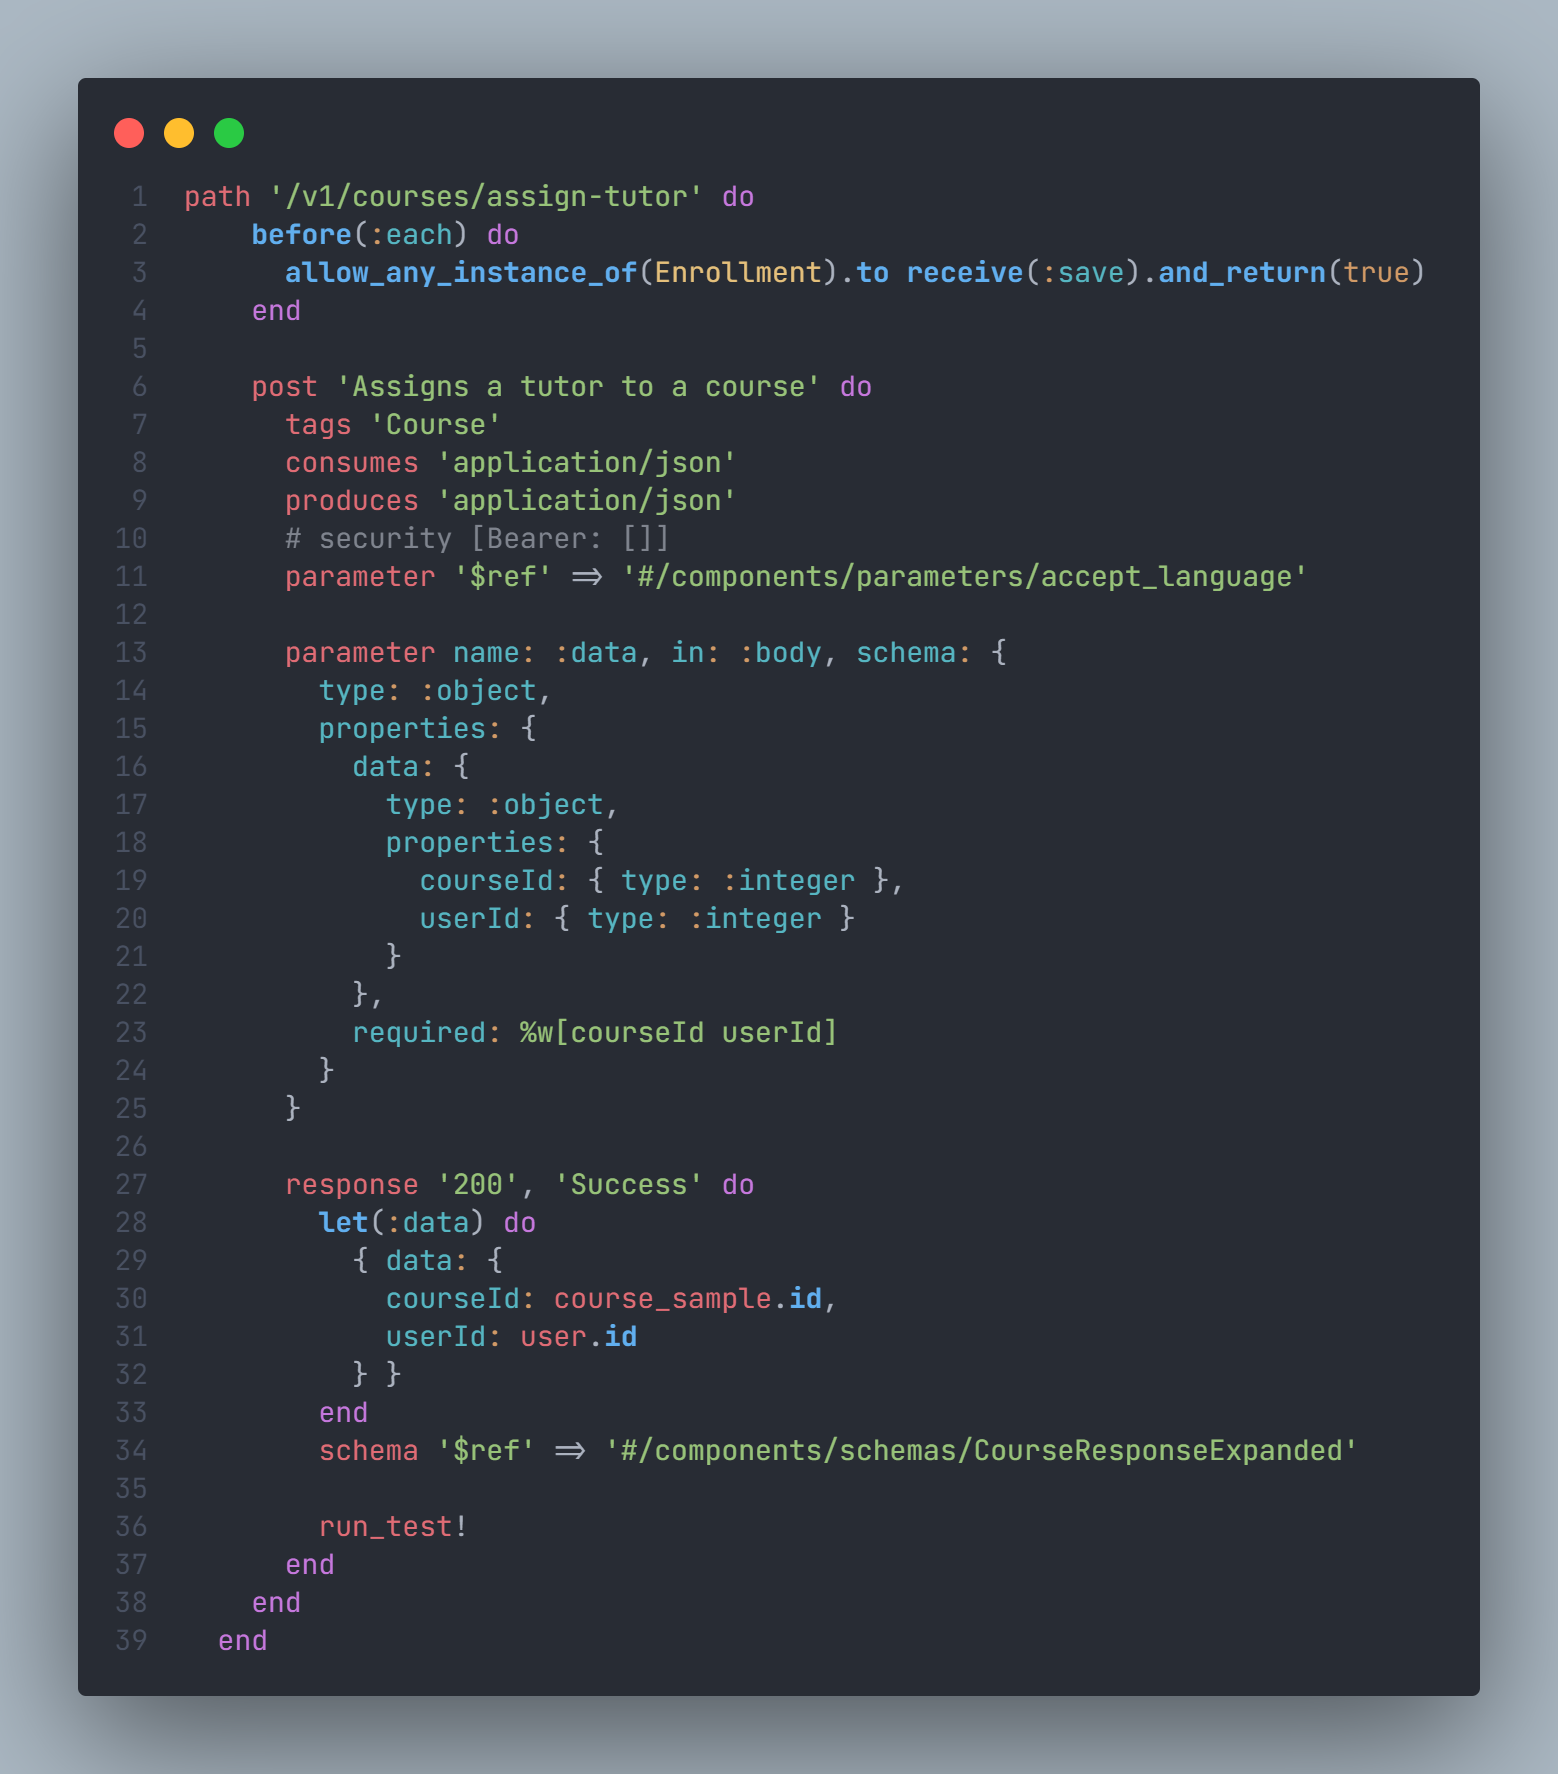
\includegraphics[width=150mm,scale=1]{figures/implementation_and_testing/testing/AIT/post_v1_courses_assign_tutor.png}}
    \caption{Course Integration Testing - Assign Tutor}
    \label{Course Integration Testing - Assign Tutor}
\end{figure}

\noindent \textbf{POST /v1/courses/assign-tutor:} This test case checks if a tutor can be assigned to a course. The courseId and userId are passed in the request body. If the tutor is successfully assigned, it should return a 200 status and the JSON object of the course with the assigned tutor.


\clearpage
\vspace{0.25cm}
\newendline \textbf{\textit{Summary}}\newendline
Integration tests ensure that specific parts of the STDC application work as intended, which improves the application's overall reliability and stability. They assisted in the prevention of errors, the acceleration of development, and the preservation of application's quality.

\end{justify}
\clearpage

%%%%%%%%%%%%%%%%%%%%%%%%%%%%%%%%%%%%%%%%%%%%%%%%%%%%%%%%%%%%%%%%%
%%%%%%%%%%%%%%%%%%%%%%%%%%%%%%%%%%%%%%%%%%%%%%%%%%%%%%%%%%%%%%%%%
%%%%%%%%%%%%%%%%%%%%%%%%%%%%%%%%%%%%%%%%%%%%%%%%%%%%%%%%%%%%%%%%%
%%%%%%%%%%%%%%%%%%%%%%%%%%%%%%%%%%%%%%%%%%%%%%%%%%%%%%%%%%%%%%%%%

\vspace{0.25cm}
\subsection{Build Verification Testing}
\begin{justify}
The purpose of build verification testing is to ensure that the STDC Web application build is functional and complies with all of the requirements. It is standard practice just before a new software version is released, build verification tests are done. The STDC's backend repository on GitHub is where the YAML file describing the CI/CD (continuous integration / continuous deployment) pipeline for the STDC can be found, and it is from there that the build verification testing is executed. Note that this test is an automated test methodology.

\vspace{0.25cm}
\newendline When a change is made to the main branch, also known as the production branch, the CI/CD pipeline is triggered. There are two jobs in the pipeline: testing and deploying. On an Ubuntu VM, the following operations constitute the Test job:

\begin{enumerate}
    \item Pulls the latest code from the main branch.
    \item Sets up the required Ruby and Node.js environments.
    \item Caches the Yarn package manager as well as Ruby gems to speed up future builds.
    \item Installs the project's dependencies using Yarn and Bundler.
    \item Runs the project's tests using the Rails test framework.
\end{enumerate}

\vspace{0.25cm}
\newendline All tests must pass before the pipeline moves on to the Deploy job, which deploys the application to production from the main branch.

\vspace{0.25cm}
\newendline There are several ways in which the application development process is improved by the build verification testing procedure:

\begin{itemize}
    \item Early discovery of problems: The practice of build verification testing assists in the early detection of problems early on in the development cycle, hence preventing those problems from being introduced into the production environment. This helps to reduce the amount of time and cost required to fix issues that could arise later.
    
    \item A shorter time required to complete the feedback loop. The CI/CD pipeline shortens the time required for developers to receive feedback on the quality of their code by automatically executing tests after each commit. This contributes to the enhancement of the code's quality as well as the reduction of the risk of introducing errors.

    \item Consistent benchmark for testing the code. This assists in increasing the quality of the code as a whole as well as eliminating conflicts amongst different version of the code base from different branches.

    \item The CI/CD pipeline automates the deployment process, which minimizes the risk of human mistake and makes the deployment process more efficient and dependable. One benefit of this automation is that the deployment process is enhanced.
\end{itemize}

\vspace{0.25cm}
\newendline In conclusion, the process of build verification testing is a vital component of the development cycle that contributes to the enhancement of the software's quality as well as the reduction of the amount of time required to resolve issues. The Continuous Integration and Continuous Deployment (CI/CD) pipeline that is supplied in the YAML file (Below here) automates the testing and deployment process. This provides the STDC development with faster feedback and a deployment procedure that is more simplified.

\begin{figure}[H]
    \centerline{\includegraphics[width=150mm,scale=1]{figures/implementation_and_testing/testing/BVT/failedtest.png}}
    \caption{Build Verification Testing - Failed Scenario}
    \label{Build Verification Testing - Failed Scenario}
\end{figure}


\begin{figure}[H]
    \centerline{\includegraphics[width=150mm,scale=1]{figures/implementation_and_testing/testing/BVT/Succeeded.png}}
    \caption{Build Verification Testing - Succeeded Scenario}
    \label{Build Verification Testing - Succeeded Scenario}
\end{figure}


\begin{figure}[H]
    \centerline{\includegraphics[width=135mm,scale=1]{figures/implementation_and_testing/testing/BVT/CICD Yaml file.png}}
    \caption{Build Verification Testing - CI/CD YAML}
    \label{Course Integration Testing - CI/CD YAML}
\end{figure}

\end{justify}
\clearpage


%%%%%%%%%%%%%%%%%%%%%%%%%%%%%%%%%%%%%%%%%%%%%%%%%%%%%%%%%%%%%%%%%
%%%%%%%%%%%%%%%%%%%%%%%%%%%%%%%%%%%%%%%%%%%%%%%%%%%%%%%%%%%%%%%%%
%%%%%%%%%%%%%%%%%%%%%%%%%%%%%%%%%%%%%%%%%%%%%%%%%%%%%%%%%%%%%%%%%
%%%%%%%%%%%%%%%%%%%%%%%%%%%%%%%%%%%%%%%%%%%%%%%%%%%%%%%%%%%%%%%%%


\vspace{0.25cm}
\subsection{Usability Testing}
\begin{justify}
Testing for usability is an essential testing methodology that serves the purpose of ensuring that a product, application, or service is user-friendly, productive, and successful for the people who are intended to use it. Testing the usability of an application entails observing and collecting feedback from users as they engage with the product or application in order to discover areas that could use improvement. The Student Talent Development Center (STDC) Web Application will undergo a usability test in order to evaluate the user experience and identify any issues that may prevent users from achieving their goals or lead to frustration and confusion. This will be accomplished by understanding how users interact with the application.

\vspace{0.25cm}
\newendline Tests of usability can be performed in a variety of ways, including in-person or remote testing, task-based or exploratory testing, expert or user testing, and more. The usability test is carried out in two stages within the framework of the STDC. Initially, participants were given the application to try out for themselves, and then, after completing the test, they were given a questionnaire to complete in order to assess the program's level of usability.

\vspace{0.25cm}
\newendline The findings of a usability test revealed some interesting and useful information on the STDC. It contributed to the identification of areas in which the designs and the user experience may be improved. Testing for usability is an iterative process; however, due to time constraints, we were only able to complete one round of testing for usability. Despite this, the findings of the test could inform us on the overall design of the application, assisting us in identifying areas that could make STDC a more user-friendly and effective application.

\vspace{0.25cm}
\newendline In general, usability testing is a vital component of the testing process, as it contributes to the development of applications that successfully satisfy the requirements of their users and deliver a satisfying experience to those users.\\


\newendline \textbf{\textit{Methodology}}\newendline
For this usability test, a survey-based approach was used to gather feedback from participants. The survey was created using Microsoft Forms and included questions that focused on the ease of use, navigation, and overall user experience of the STDC application. The survey was distributed to a convenience sample of at least 08 participants who were selected based on their familiarity with the subject matter and potential use of the application.

\vspace{0.25cm}
\newendline Participants were asked to complete the survey based on their experience using the STDC application, which they accessed via a provided link. Participants were given approximately 15 minutes to complete the survey and an additional 30 to 60 mins to completely test the application.

\vspace{0.25cm}
\newendline The survey consisted of closed and open-ended questions. Closed-ended questions used a scale to measure the level of agreement or disagreement with statements related to the usability of the application. Open-ended questions allowed participants to provide more detailed feedback about specific aspects of the application that they found challenging or easy to use.

\vspace{0.25cm}
\newendline After the survey data was collected, the results were analyzed to identify common themes and issues that emerged across participants. Both quantitative and qualitative methods were used to analyze the data.

\vspace{0.25cm}
\newendline While we recognize that survey-based approaches may not capture all aspects of the user experience, we felt that it was a practical approach given our time constraints and the need to gather feedback from a diverse group of participants.\\


\newendline \textbf{\textit{Participants}}\newendline
The survey was distributed to a convenience sample of at least 08 participants who were selected based on their familiarity with the subject matter and potential use of the application. Additionally, participants with higher tech-savviness were more favorable to be chose as participants to test the application.

\vspace{0.25cm}
\newendline Also due to the small number of staff at the STDC, only one participant who is a staff was able to test the application.


\newendline \textbf{\textit{Tasks}}\newendline
The usability test is carried out in two stages within the framework of the STDC. Initially, participants were given the application to try out for themselves, and then, after completing the test, they were given a questionnaire to complete in order to assess the program's level of usability.


\newendline \textbf{\textit{Questionnaires}}\newendline
The followings are the questions of the survey/questionnaire that were asked from the participants.

\begin{figure}[H]
    \centerline{\includegraphics[width=150mm,scale=1]{figures/implementation_and_testing/testing/MUT/questions/Questions (1).png}}
    \caption{Usability Testing Questionnaires - Guide}
    \label{Usability Testing Questionnaires - Guide}
\end{figure}

\begin{figure}[H]
    \centerline{\includegraphics[width=150mm,scale=1]{figures/implementation_and_testing/testing/MUT/questions/Questions (2).png}}
    \caption{Usability Testing Questionnaires - Section I}
    \label{Usability Testing Questionnaires - Section I}
\end{figure}

\begin{figure}[H]
    \centerline{\includegraphics[width=150mm,scale=1]{figures/implementation_and_testing/testing/MUT/questions/Questions (3).png}}
    \caption{Usability Testing Questionnaires - Section II (1)}
    \label{Usability Testing Questionnaires - Section II (1)}
\end{figure}

\begin{figure}[H]
    \centerline{\includegraphics[width=150mm,scale=1]{figures/implementation_and_testing/testing/MUT/questions/Questions (4).png}}
    \caption{Usability Testing Questionnaires - Section II (2)}
    \label{Usability Testing Questionnaires - Section II (2)}
\end{figure}

\begin{figure}[H]
    \centerline{\includegraphics[width=150mm,scale=1]{figures/implementation_and_testing/testing/MUT/questions/Questions (5).png}}
    \caption{Usability Testing Questionnaires - Section II (3)}
    \label{Usability Testing Questionnaires - Section II (3)}
\end{figure}

\begin{figure}[H]
    \centerline{\includegraphics[width=150mm,scale=1]{figures/implementation_and_testing/testing/MUT/questions/Questions (6).png}}
    \caption{Usability Testing Questionnaires - Section II (4)}
    \label{Usability Testing Questionnaires - Section II (4)}
\end{figure}

\begin{figure}[H]
    \centerline{\includegraphics[width=150mm,scale=1]{figures/implementation_and_testing/testing/MUT/questions/Questions (7).png}}
    \caption{Usability Testing Questionnaires - Section II (5)}
    \label{Usability Testing Questionnaires - Section II (5)}
\end{figure}

\begin{figure}[H]
    \centerline{\includegraphics[width=150mm,scale=1]{figures/implementation_and_testing/testing/MUT/questions/Questions (8).png}}
    \caption{Usability Testing Questionnaires - Section II (6)}
    \label{Usability Testing Questionnaires - Section II (6)}
\end{figure}

\begin{figure}[H]
    \centerline{\includegraphics[width=150mm,scale=1]{figures/implementation_and_testing/testing/MUT/questions/Questions (9).png}}
    \caption{Usability Testing Questionnaires - Section II (7)}
    \label{Usability Testing Questionnaires - Section II (7)}
\end{figure}

\clearpage
\newendline \textbf{\textit{Results and Analysis}}\newendline
Below here is a brief analysis of the result of each question. It is worth noting that not all the details may have been highlighted.

\vspace{0.25cm}
\newendline \textbf{Question 1:} Have you tested the application?

\begin{figure}[H]
    \centerline{\includegraphics[width=150mm,scale=1]{figures/implementation_and_testing/testing/MUT/answers/Answers (1).png}}
    \caption{Usability Testing Results - Question 1}
    \label{Usability Testing Results - Question 1}
\end{figure}

\vspace{0.25cm}
\newendline 100\% of participants tested the application, this indicates that all responses given are based on actual usage experience and also it provides valuable feedback on the usability of the application.\\

\vspace{0.25cm}
\newendline \textbf{Question 2:} What is your current occupation?

\begin{figure}[H]
    \centerline{\includegraphics[width=150mm,scale=1]{figures/implementation_and_testing/testing/MUT/answers/Answers (2).png}}
    \caption{Usability Testing Results - Question 2}
    \label{Usability Testing Results - Question 2}
\end{figure}

\vspace{-0.25cm}
\newendline Most of the participants are students, with only one participant identifying as a Staff / Admin. This gives a good perspective from the main user base (students), but the limited feedback from staff/admin may not fully represent their experience.

\vspace{0.25cm}
\newendline \textbf{Question 3:} How would you rate your level of confidence in using your mobile phone / personal computer for browsing the internet?

\begin{figure}[H]
    \centerline{\includegraphics[width=150mm,scale=1]{figures/implementation_and_testing/testing/MUT/answers/Answers (3).png}}
    \caption{Usability Testing Results - Question 3}
    \label{Usability Testing Results - Question 3}
\end{figure}

\vspace{0.25cm}
\newendline The majority of participants rated their level of confidence as very high (9 or 10). This indicates that the user base is tech-savvy and comfortable using digital platforms. The average rating of 9.0 suggests that most issues identified during the testing are likely related to the application itself rather than a lack of technical skills from the users.\\

\vspace{-0.25cm}
\newendline \textbf{Question 4:} Have you previously heard about the Student Talent Development Center? If yes, how have you interacted with STDC?

\begin{figure}[H]
    \centerline{\includegraphics[width=150mm,scale=1]{figures/implementation_and_testing/testing/MUT/answers/Answers (4).png}}
    \caption{Usability Testing Results - Question 4}
    \label{Usability Testing Results - Question 4}
\end{figure}

\vspace{0.25cm}
\newendline Most participants were aware of the STDC's existence but had not engaged with it. This shows that while the STDC has visibility, it might need to work on its engagement strategies to better reach and interact with its potential students which in a way indicates the importance of this system.

\vspace{0.25cm}
\newendline \textbf{Question 5:} What device did you use for testing STDC web application?

\begin{figure}[H]
    \centerline{\includegraphics[width=150mm,scale=1]{figures/implementation_and_testing/testing/MUT/answers/Answers (5).png}}
    \caption{Usability Testing Results - Question 5}
    \label{Usability Testing Results - Question 5}
\end{figure}

\vspace{-0.25cm}
\newendline Most participants used a Laptop/PC to test the application. This information could be used to prioritize design and functionality aspects tailored towards desktop users in the future.\\


\vspace{0.25cm}
\newendline \textbf{Question 6:} How easy or difficult was it to sign up for the application?

\begin{figure}[H]
    \centerline{\includegraphics[width=150mm,scale=1]{figures/implementation_and_testing/testing/MUT/answers/Answers (6).png}}
    \caption{Usability Testing Results - Question 6}
    \label{Usability Testing Results - Question 6}
\end{figure}

\vspace{-0.25cm}
\newendline Most participants found it not difficult to sign up, suggesting the sign up process is intuitive and user friendly, however there are concerns still regarding the sign up which we will talk about in details in the next section (Recommendations).


\vspace{0.25cm}
\newendline \textbf{Question 7:} How easy or difficult was it to navigate through the application? 

\begin{figure}[H]
    \centerline{\includegraphics[width=150mm,scale=1]{figures/implementation_and_testing/testing/MUT/answers/Answers (7).png}}
    \caption{Usability Testing Results - Question 7}
    \label{Usability Testing Results - Question 7}
\end{figure}

\vspace{0.25cm}
\newendline Overall, participants found the application relatively easy to navigate. This indicates the application’s layout and navigation structure are well designed.\\

\vspace{0.25cm}
\newendline \textbf{Question 8:} What are your thoughts on the design and layout?

\begin{figure}[H]
    \centerline{\includegraphics[width=150mm,scale=1]{figures/implementation_and_testing/testing/MUT/answers/Answers (8).png}}
    \caption{Usability Testing Results - Question 8}
    \label{Usability Testing Results - Question 8}
\end{figure}

\vspace{0.25cm}
\newendline Most participants found the design appealing and easy to use. However, a minority suggested that it could benefit from usability improvements. This might indicate some minor issues that could be smoothed out to further enhance the user experience for which more details need to be collected from the users to see what are the specific issues.\\

\vspace{0.25cm}
\newendline \textbf{Question 9:} On the scale of (1..10), how did you find the information provided by the application? 

\begin{figure}[H]
    \centerline{\includegraphics[width=150mm,scale=1]{figures/implementation_and_testing/testing/MUT/answers/Answers (9).png}}
    \caption{Usability Testing Results - Question 9}
    \label{Usability Testing Results - Question 9}
\end{figure}

\vspace{-0.25cm}
\newendline The high average rating indicates that participants found the information provided by the application to be useful and adequate.\\


\vspace{0.25cm}
\newendline \textbf{Question 10:} How easy was it to find the available courses and sessions?

\begin{figure}[H]
    \centerline{\includegraphics[width=150mm,scale=1]{figures/implementation_and_testing/testing/MUT/answers/Answers (10).png}}
    \caption{Usability Testing Results - Question 10}
    \label{Usability Testing Results - Question 10}
\end{figure}

\vspace{0.25cm}
\newendline Most participants found it extremely easy to find the available courses and sessions, indicating that these key features are accessible and well-implemented.

\vspace{0.25cm}
\newendline \textbf{Question 11:} How difficult was it to find time and venue for a session?

\begin{figure}[H]
    \centerline{\includegraphics[width=150mm,scale=1]{figures/implementation_and_testing/testing/MUT/answers/Answers (11).png}}
    \caption{Usability Testing Results - Question 11}
    \label{Usability Testing Results - Question 11}
\end{figure}

\vspace{0.25cm}
\newendline  Most participants did not find it difficult to find the time and venue for a session, implying that this aspect of the application is well designed.\\


\vspace{0.25cm}
\newendline \textbf{Question 12:} How did you feel about providing feedback about sessions?

\begin{figure}[H]
    \centerline{\includegraphics[width=150mm,scale=1]{figures/implementation_and_testing/testing/MUT/answers/Answers (12).png}}
    \caption{Usability Testing Results - Question 12}
    \label{Usability Testing Results - Question 12}
\end{figure}

\vspace{0.25cm}
\newendline All participants felt confident or very confident in providing feedback about sessions. This shows that the feedback system is intuitive and user-friendly.\\


\clearpage

\vspace{0.25cm}
\newendline \textbf{Question 13:} How would you describe your overall experience?

\begin{figure}[H]
    \centerline{\includegraphics[width=150mm,scale=1]{figures/implementation_and_testing/testing/MUT/answers/Answers (13).png}}
    \caption{Usability Testing Results - Question 13}
    \label{Usability Testing Results - Question 13}
\end{figure}

\vspace{0.25cm}
\newendline With an average rating of 8.44, participants had a positive overall experience with the application.\\

\clearpage
\vspace{0.25cm}
\newendline \textbf{Question 14:} What did you like the most about using this product?

\begin{figure}[H]
    \centerline{\includegraphics[width=150mm,scale=1]{figures/implementation_and_testing/testing/MUT/answers/Answers (14).png}}
    \caption{Usability Testing Results - Question 14}
    \label{Usability Testing Results - Question 14}
\end{figure}

\vspace{0.25cm}
\newendline Participants particularly highlighted the ease of use the design that they liked the most..\\

\clearpage
\vspace{0.25cm}
\newendline \textbf{Question 15:} How can you increase the product’s ease of use?

\begin{figure}[H]
    \centerline{\includegraphics[width=150mm,scale=1]{figures/implementation_and_testing/testing/MUT/answers/Answers (15).png}}
    \caption{Usability Testing Results - Question 15}
    \label{Usability Testing Results - Question 15}
\end{figure}

\vspace{0.25cm}
\newendline A few participants suggested the inclusion of more back and forward access buttons to improve navigation which seem to be missing from the application.


\clearpage
\vspace{0.25cm}
\newendline \textbf{Question 16:} What did you like the least about using this product?

\begin{figure}[H]
    \centerline{\includegraphics[width=150mm,scale=1]{figures/implementation_and_testing/testing/MUT/answers/Answers (16).png}}
    \caption{Usability Testing Results - Question 16}
    \label{Usability Testing Results - Question 16}
\end{figure}

\vspace{0.25cm}
\newendline There were mixed responses, but one participant indicated issues with signing up. This could imply a possible area of improvement, although most other participants had no issues with the sign-up process.\\

\clearpage
\vspace{0.25cm}
\newendline \textbf{Question 17:} What, if anything, caused you frustration?

\begin{figure}[H]
    \centerline{\includegraphics[width=150mm,scale=1]{figures/implementation_and_testing/testing/MUT/answers/Answers (17).png}}
    \caption{Usability Testing Results - Question 17}
    \label{Usability Testing Results - Question 17}
\end{figure}

\vspace{0.25cm}
\newendline Most participants did not report any frustrations with the application, suggesting a generally positive user experience.\newendline
Please Note that the fact that not all participants answered these open-ended questions indicates that they may have found it challenging to articulate specific points, or that the questions could have been clearer.\\

\clearpage
\newendline \textbf{\textit{Recommendations}}\newendline
Based on the findings of the usability tests, numerous suggestions for improving the STDC Web Application's usability have been formulated. These suggestions, which are based on both quantitative and qualitative data from the survey, are meant to enhance the usability of the app, boost user engagement, and boost satisfaction.

\vspace{0.25cm}
\newendline To begin, it is suggested that a desktop-friendly interface be given high priority during the future design and development of the STDC web application’s new versions because that is how the vast majority of users accessed the service. The desktop is the major access point for the user base, thus while the application should stay responsive and compatible with mobile devices, it should primarily focus on maximizing the desktop user experience.

\vspace{0.25cm}
\newendline While the vast majority of users had no problems signing up, comments from a subset of users indicate that this step may use some tweaking. It could be useful to have a look over the signup procedure and see if there are any places where people get stuck or where the instructions aren't clear. In addition, a user-friendly, detailed guidance to the sign-up procedure could facilitate the first step for new customers.

\vspace{0.25cm}
\newendline While users generally had a positive experience with the app, some provided constructive criticism suggesting that more back and move forward buttons may be helpful. By giving consumers more say over how they navigate, this feature has a high potential to improve the usability of the interface.

\vspace{0.25cm}
\newendline The majority of users found the application's interface to be intuitive and simple to operate, while a few pointed out that the program should be made more user-friendly. This suggests that the user interface and usability could benefit from additional development work. The user experience might be improved through the use of current design principles, UI best practices, and elements like user-friendly iconography, consistent typography, and a clear information hierarchy.

\vspace{0.25cm}
\newendline Participants gave the app good marks for the quality of the information it supplied. However, reviews at periodic times are necessary to keep the content fresh, accurate, and presented in a way that is simple to understand and absorb by readers. It also would be helpful to provide users with a 'help' or 'FAQ' page that answers frequently asked questions and provides further information on how to use the app.

\vspace{0.25cm}
\newendline User response was generally positive, and all testers felt comfortable using the application's built-in feedback system. However, the STDC may want to think about creating mechanisms to actively encourage feedback input in order to generate even higher engagement. Users can be encouraged to provide feedback by means of reminders, prompts, and even a rewards system.

\vspace{0.25cm}
\newendline Users had a generally favorable experience, giving these features high marks. However, a commitment to iteration and improvement based on user input is necessary as application development is an ongoing process. Conducting usability testing on a regular basis can assist find more problem areas and make sure the app keeps evolving to suit users' requirements and expectations. Nevertheless due to the time constraints only one round of testing could be done.

\vspace{0.25cm}
\newendline In conclusion, while the STDC online application is functional as it stands, it has room for improvement that might make it even more accessible, intuitive, and interesting to use. The STDC web application has the potential to become an even more efficient and helpful resource for its users through consistent assessment, the incorporation of user feedback, and awareness of technological advancements.


\end{justify}
\clearpage


%%%%%%%%%%%%%%%%%%%%%%%%%%%%%%%%%%%%%%%%%%%%%%%%%%%%%%%%%%%%%%%%%
%%%%%%%%%%%%%%%%%%%%%%%%%%%%%%%%%%%%%%%%%%%%%%%%%%%%%%%%%%%%%%%%%
%%%%%%%%%%%%%%%%%%%%%%%%%%%%%%%%%%%%%%%%%%%%%%%%%%%%%%%%%%%%%%%%%
%%%%%%%%%%%%%%%%%%%%%%%%%%%%%%%%%%%%%%%%%%%%%%%%%%%%%%%%%%%%%%%%%


\vspace{0.25cm}
\subsection{User Acceptance Testing}
\begin{justify}
The User Acceptance Test (UAT) serves as the final phase of testing for the Student Talent Development Center (STDC) web application. This crucial step ensures that the application meets the requirements and expectations of its users. As the UAT is the last testing phase, it plays a vital role in validating the application's readiness for deployment.

\vspace{0.25cm}
\newendline Considering the project timeline and constraints, it was not possible to involve the end users or stakeholders directly in the UAT process. Therefore, this UAT will be conducted by myself. This implies that the testing will be conducted in an alpha environment.

\vspace{0.25cm}
\newendline The purpose of this document is to outline the chosen criteria for the UAT, present the test results in a structured manner, and provide a conclusion to the UAT phase.

\vspace{0.25cm}
\newendline \textbf{\textit{Criteria}}\newendline
In selecting the criteria for the User Acceptance Test, several factors were considered. Firstly, the successful completion of previous testing phases, including inspection testing, automated unit testing, automated integration testing, build verification testing, boundary analysis testing, and usability testing, serves as an indicator of the application's stability.

\vspace{0.25cm}
\newendline Additionally, the Requirements Traceability Matrix (RTM) and Test Case tables were used as primary criteria for the UAT. The RTM ensures that all requirements have corresponding test cases, while the Test Case tables indicate the successful completion of each test case.

\vspace{0.25cm}
\newendline Furthermore, it is worth noting that the usability testing conducted for the STDC web app yielded positive feedback, please refer back to the previous sections.

\vspace{0.25cm}
\newendline \textbf{\textit{UAT Results}}\newendline
The following table provides an overview of the requirements and their corresponding status after conducting the User Acceptance Test. The following is the column descriptions:

\begin{itemize}
    \item \textbf{RQ. ID:} Requirement ID.
    \item \textbf{Acceptance Criteria:} The specific criteria that need to be met for each requirement to be considered accepted.
    \item \textbf{Critical:} Indicates whether a requirement is critical or not.
    \item \textbf{Test Status:} The current status of each requirement based on the testing conducted.
    \item \textbf{UAT Result:} The result of the User Acceptance Test for each requirement, indicating whether it was accepted or not.\\
\end{itemize}



\renewcommand{\arraystretch}{1.0}
\begin{longtable}[c]{|p{1.5cm}|p{5cm}|p{1.75cm}|p{2.5cm}|p{2.5cm}|}
\caption{Requirements Testing Table} \\
\hline
\textbf{RQ. ID} & \textbf{Acceptance Criteria} & \textbf{Critical} & \textbf{Test Status} & \textbf{UAT Result} \\
\hline
\endfirsthead
\multicolumn{5}{c}%
{\tablename\ \thetable\ -- \textit{Continued from previous page}} \\
\hline
\textbf{RQ. ID} & \textbf{Acceptance Criteria} & \textbf{Critical} & \textbf{Test Status} & \textbf{UAT Result} \\
\hline
\endhead
\hline \multicolumn{5}{|c|}{\textit{Continued on next page}} \\ \hline
\endfoot
\hline
\endlastfoot
RQ01 & All users must be able to login using UKH email and password. & Yes & Passed & Accepted \\
\hline
RQ02 & Tutors must be able to enter attendance for each session. & Yes & Passed & Accepted \\
\hline
RQ03 & All users must be able to list courses taught in STDC. Current user's courses should appear on top. & Yes & Passed & Accepted \\
\hline
RQ04 & All users must be able to view an individual course. & Yes & Passed & Accepted \\
\hline
RQ05 & Admin must be able to create a new course. & Yes & Passed & Accepted \\
\hline
RQ06 & Admin must be able to update a course. & Yes & Passed & Accepted \\
\hline
RQ07 & Admin must be able to delete a course. & Yes & Passed & Accepted \\
\hline
RQ08 & All users must be able to list sessions. & Yes & Passed & Accepted \\
\hline
RQ09 & All users must be able to view an individual session. & Yes & Passed & Accepted \\
\hline
RQ10 & Admin must be able to create a new session. & Yes & Passed & Accepted \\
\hline
RQ11 & Admin must be able to update an existing session. & Yes & Passed & Accepted \\
\hline
RQ12 & Admin must be able to delete an existing session. & Yes & Passed & Accepted \\
\hline
RQ13 & Admin must be able to list venues. & Yes & Passed & Accepted \\
\hline
RQ14 & All users must be able to view an individual venue. & Yes & Passed & Accepted \\
\hline
RQ15 & Admin must be able to create (register) a new venue. & Yes & Passed & Accepted \\
\hline
RQ16 & Admin must be able to update an existing venue. & Yes & Passed & Accepted \\
\hline
RQ17 & Admin must be able to delete an existing venue. & Yes & Passed & Accepted \\
\hline
RQ18 & Admin must be able to onboard tutors. & Yes & Passed & Accepted \\
\hline
RQ19 & Admin must be able to assign tutors to courses. & Yes & Passed & Accepted \\
\hline
RQ20 & Tutors should be able to update their profiles. & Yes & Passed & Accepted \\
\hline
RQ21 & Admin and tutors should be able to view the attendance statistics of a student. & Yes & Passed & Accepted \\
\hline
RQ22 & Tutors should be able to list all students in a course. & Yes & Passed & Accepted \\
\hline
RQ23 & Tutors should be able to view the profile of a student. & Yes & Passed & Accepted \\
\hline
RQ24 & Tutors should be able to view a student's progress and assignments. & No & Passed & Accepted \\
\hline
RQ25 & Admin must be able to create a course schedule for each semester. & Yes & Passed & Accepted \\
\hline
RQ26 & Admin must be able to update a course schedule. & Yes & Passed & Accepted \\
\hline
RQ27 & Admin must be able to delete a course schedule. & Yes & Passed & Accepted \\
\hline
RQ28 & Tutors should be able to grade students for each course. & No & Passed & Accepted\\
\hline
RQ29 & All users should be able to access materials uploaded. & No & Passed & Accepted\\
\hline
RQ30 & Tutors should be able to upload files (materials) for a given session of a course. & No & Passed & Accepted \\
\hline
\end{longtable}


\vspace{0.5cm}
\newendline \textbf{\textit{Summary}}\newendline
In conclusion, the User Acceptance Test (UAT) for the Student Talent Development Center (STDC) web app has been conducted successfully. By leveraging the criteria set forth, including the RTM, Test Case tables, and positive usability feedback, the UAT aimed to validate the application's compliance with user expectations.

\vspace{0.25cm}
\newendline The UAT results indicate that all requirements have been tested and met, as evidenced by the successful completion of the UAT Table. This outcome provides confidence in the readiness of the STDC web app for deployment.

\vspace{0.25cm}
\newendline With the completion of the UAT, the project can now move forward to the next phase with the assurance that the application has undergone thorough testing, fulfilling the necessary quality standards.

\end{justify}
\clearpage

